\documentclass[11pt, a5paper]{article}

\usepackage[T2A]{fontenc}
\usepackage[utf8]{inputenc}
\usepackage[english, russian]{babel}
\usepackage{amssymb, amsfonts, amsmath}
\usepackage{mathtext}
\usepackage{comment}
\usepackage{graphicx}
\usepackage{listings}
\usepackage{geometry}
\usepackage{lscape}
\usepackage{wrapfig}
\usepackage[indentfirst, pagestyles, explicit]{titlesec}
\usepackage{longtable}

\usepackage{tikz}
\usetikzlibrary{patterns}		%draw pictures: fill
\usetikzlibrary{calc}			%draw pictures: coordinate calc
% \usetikzlibrary{external}		%draw pictures: cache pitcures
% \tikzexternalize				%cache pictures
\usepackage{listofitems}		%list of arguments (pictures)
\usepackage{enumitem}			%enumarate parameters

\geometry{left=1cm, right=1cm, top=2cm, bottom=2cm, twoside}

\titleformat{\section}{\Large\bfseries\center}{}{0pt}{#1}
\titleformat{\subsection}{\Large\bfseries\center}{}{0pt}{#1}

\newpagestyle{mystyle}{
	\headrule
	\sethead[\sectiontitle][][]
			{}{}{\subsectiontitle}
	\setfoot[\thepage][][]
			{}{}{\thepage}
}

\lstset{language=C++}
\lstset{basicstyle=\footnotesize\ttfamily} 
\lstset{keywordstyle=\color{blue}}
\lstset{frame=single}
\lstset{numbers=left}

\sloppy

\newcommand{\accept}[2]{
	\centerline{\boxed{#1}}
	\newline
	\centerline{\scriptsize{#2}}
}
\newcommand{\reject}[1]{
	\centerline{#1}
}

\newcommand{\informat}[1]
{
	\paragraph{Ввод.\\} #1
}

\newcommand{\outformat}[1]
{
	\paragraph{Вывод.\\} #1
}

\newcommand{\example}[2]
{
	\paragraph{Пример.\\}
	{\tt
	\begin{tabular}{|p{0.4\linewidth}|p{0.4\linewidth}|}
	\hline
	Ввод & Вывод \\
	\hline
	#1 & #2		\\
	\hline
	\end{tabular}
	}
}

\newcommand{\examplee}[4]
{
	\paragraph{Пример.\\}
	{\tt
	\begin{tabular}{|p{0.4\linewidth}|p{0.4\linewidth}|}
	\hline
	Ввод 	& Вывод  	\\
	\hline
	#1 		& #2 		\\
	\hline
	#3		& #4		\\
	\hline
	\end{tabular}
	}
}

\newcommand{\examplEEE}[6]
{
	\paragraph{Пример.\\}
	{\tt
	\begin{tabular}{|p{0.5\linewidth}|p{0.3\linewidth}|}
	\hline
	Ввод 	& Вывод  	\\
	\hline
	#1 		& #2 		\\
	\hline
	#3		& #4		\\
	\hline
	#5		& #6		\\
	\hline
	\end{tabular}
	}
}

\newcommand{\exampleee}[6]
{
	\paragraph{Пример.\\}
	{\tt
	\begin{tabular}{|p{0.4\linewidth}|p{0.4\linewidth}|}
	\hline
	Ввод 	& Вывод  	\\
	\hline
	#1 		& #2 		\\
	\hline
	#3		& #4		\\
	\hline
	#5		& #6		\\
	\hline
	\end{tabular}
	}
}

\newcommand{\exampleeee}[8]
{
	\paragraph{Пример.\\}
	{\tt
	\begin{tabular}{|p{0.4\linewidth}|p{0.4\linewidth}|}
	\hline
	Ввод 	& Вывод  	\\
	\hline
	#1 		& #2 		\\
	\hline
	#3		& #4		\\
	\hline
	#5		& #6		\\
	\hline
	#7		& #8		\\
	\hline
	\end{tabular}
	}
}

\newcommand{\exampleeeee}[5]
{
	\paragraph{Пример.\\}
	{\tt
	\begin{tabular}{|p{0.4\linewidth}|p{0.4\linewidth}|}
	\hline
	Ввод 	& Вывод  	\\
	\hline
	#1		\\
	\hline
	#2		\\
	\hline
	#3		\\
	\hline
	#4		\\
	\hline
	#5		\\
	\hline
	\end{tabular}
	}
}

\newcommand{\examplepic}[3]
{
	\subsection*{Пример.}
	{\tt
	\noindent
	\begin{tabular}{|p{0.1\linewidth}|p{0.1\linewidth}|p{0.5\linewidth}|}
	\hline
	Ввод 	& Вывод  	& Пояснение\\
	\hline
	#1 		& #2 		& #3\\
	\hline
	\end{tabular}
	}
}


\newcommand{\excomm}[1]
{
	\paragraph{Комментарий. \\}
	\textit{#1}
}

\renewcommand{\tabcolsep}{0.1cm}
\def\arraystretch{2}

\newcommand{\result}[2]
{
	\begin{landscape}
	\begin{center}

	\begin{large}
		Результаты\\
		#2\\
		\vspace{0.5cm}
	\end{large}	
	
	\begin{tiny}
	\input{results/#1}
	\end{tiny}
	\end{center}
	\end{landscape}
	\newpage
}
\newcommand{\resultind}[2]
{
	\newpage
	\begin{center}

	\begin{large}
		Результаты\\
		#2\\
		\vspace{0.5cm}
	\end{large}	
	
	\begin{tiny}
	\input{results/#1}
	\end{tiny}
	\end{center}
	\newpage
}

\newcommand{\problemauthor}[1]{
\begin{flushright}
\textit{Автор: #1}
\end{flushright}
}

\newcommand{\problemofferer}[1]{
\begin{flushright}
\textit{Предложил: #1}
\end{flushright}
}

\newcommand{\head}[2]
{
    \subsection{#1}
    \begin{center}
	#2
	\end{center}
}


\begin{document}

\begin{titlepage}
\begin{center}
\vfill

Московский государственный университет имени М.В.~Ломоносова\\
Казахстанский филиал\\

\vfill

\begin{Large}
\textbf{Студенческие олимпиады по программированию\\
Казахстанского филиала МГУ. \\
Задачи и указания.\\
2013--2018 гг.\\
}
\end{Large}

\vfill

Астана\\
2018

\end{center}
\end{titlepage}

\setcounter{page}{2}


\thispagestyle{empty}

\noindent{\bf УДК} \\
{\bf ББК}\\
{\bf Л}
\vspace{0.7 cm}

{\bf Рецензент:}

кандидат физико--математических наук, доцент кафедры математики и информатики Казахстанского филиала МГУ имени М.~В.~Ломоносова Нетесов~В.~В.

\vspace{0.5 cm}

{\bf Авторы:}

преподаватели Казахстанского филиал МГУ имени М.~В.~Ломоносова Абдикалыков~А.~К., Баев~А.~Ж.

\vspace{0.5 cm}

{\bf TeX--верстка:}

Баев~А.~Ж.

\vspace{0.5 cm}

В настоящем сборнике представлены 113 задач с указаниями, которые предлагались на 13 студенческих олимпиадах по программированию Казахстанского филиала МГУ имени М.В.Ломоносова за период с 2013 по 2018 год. 

Сборник  адресован  всем интересующимся олимпиадным движением.

\vspace{0.5 cm}


{\bf ISBN}  

\newpage
\section{Предисловие}

Традиция ежегодных студенческих олимпиад Казахстанского филиала МГУ по программированию зародилась со дня открытия филиала в 2001 году. Олимпиады проводились один раз в год в декабре при непосредственном участии доцента кафедры математики и информатики Казахстанского филиала МГУ Нетесова Виктора Викторовича и удаленном участии доцента кафедры системного программирования факультета ВМК Чернова Александра Владимировича, который является автором известной системы для проведения олимпиад по программированию ejudge. 

С 2013-2014 учебного года олимпиада разделилась на весенний и осенний тур с командным участием, а в 2015-2016 учебном году добавился индивидуальный тур с индивидуальным участием. С 2015 года олимпиада проводится с онлайн--версией, что позволяет принять участие в олимпиаде участникам из других городов, в частности студентам 3--4 курса Казахстанского филиала МГУ, которые обучаются в Москве. За последние годы в олимпиаде принимали участие студенты учебных заведений Казахстана (Астана, Алматы) и городов других стран (Москва, Ташкент).

В данном сборнике содержится 113 задач, которые были предложены на девяти олимпиадах филиала МГУ в период с 2013 по 2018 год. Значительная часть задач была разработана и подготовлена преподавателями Казахстанского филиала МГУ имени М.В.~Ломоносова Абдикалыковым Абдикожой Кожанасиридиновичем и Баевым Аленом Жуматаевичем. 

Активное участие в подготовке олимпиад принимали и самми студенты. Так, большую помощь в организации олимпиады 2012 года оказал студент четвертого курса ВМК Максимец Илья. Зимний тур 2015 года подготовили студенты второго курса: Камалбеков Тимур, Журавская Александра, Абайулы Ерулан и Жусупов Али. А зимний тур 2017 года: Аскергалиев Ануар, Бекмаганбетов Бекарыс и Шарипов Азат.

Авторы выражают благодарность всем студентам, кто принимал участие в олимпиадах филиала.

\begin{flushright}
Директор Казахстанского филиала

А.В.Сидорович
\end{flushright}

\newpage

\pagestyle{mystyle}

\tableofcontents

\newpage

\section{Команды Филиала на чемпионате ACM~ICPC}

В текстах задач олимпиад Казахстанского филиала упоминаются студенты, которые активно участвовали в олимпиадном движении филиала в период с 2012 по 2017 год и, в частности, принимали участие в чемпионате мира по программированию ACM ICPC.

Чемпионат мира по программированию проводится в несколько этапов. Четвертьфинал чемпионата мира для команд из Казахстана проводится параллельно в Алматы и Астане в конце октября. Обычно он собирает около 100 команд, представляющих около 30 университетов Казахстана. Около 30 лучших команд (но не более 4 команд из одного университета) приглашаются на следующий этап --- полуфинал чемпионата мира.

Команды, отобранные на 16 четвертьфиналах Северо-Восточного Европейского региона, встречаются на полуфинале в начале декабря. Соревнование проводится параллельно на одном и том же наборе задач сразу на четырех площадках: Ташкент (до 2015 года), Алматы (с 2016 года), Барнаул, Тбилиси и Санкт-Петербург. Как правило, это около 240 команд, представляющие 120 ВУЗов данного региона. Около 15 лучших команд (но не более 1 команды из одного университета) приглашаются на финал.

Всего за 6 сезонов с 2012 по 2017 год в четвертьфинале команды представляли филиал 21 раз, из которых 17 раз успешно квалифицировались на полуфинал. Команда филиала принимала участие в полуфинале на трех разных площадках: г. Ташкент в 2012 году, г. Барнаул в 2013 и 2015 годах и г. Алматы в 2016 и в 2017 годах. Лучшим достижением команд филиала на полуфинале является дипломы Средней Азии (г. Ташкент, 2012), Сибири (г. Барнаул, 2015), Северо-Восточного Европейского региона (г. Алматы, 2016).

Команды филиала состоят из студентов, обучающихся по направлениям <<Математика>> и <<Прикладная математика>>. Многие участники команд филиала знакомятся с олимпиадами по програмированию в течении первого года обучения. Уже ко второму курсу они часто выступают на равных с опытными соперниками из других ВУЗов Казахстана.

Условия задач, результаты и материалы четвертьфиналов и полуфинала чемпионата мира по программированию ACM ICPC доступны на официальном сайте организатора в лице Санкт-Петербургского национального исследовательского университета информационных технологий, механики и оптики: https://neerc.ifmo.ru.

\subsubsection*{2012--2013 учебный год}

\paragraph{Четвертьфинал чемпионата (Казахстан).} Казахстанский филиал МГУ занял 6 место из 28 ВУЗов Казахстана, а лучшая команда филиала --- 22 место из 110 команд.

\paragraph{Полуфинал чемпионата (Средняя Азии).} Казахстанский филиал МГУ занял 11 место из 18 ВУЗов Средней Азии, а лучшая команда филиала --- 22 место из 47 команд Средней Азии (15 место из 29 среди команд из Казахстана). Данный результат отмечен \textbf{дипломом третьей степени среди команд Казахстана}.

\paragraph{Полуфинал чемпионата (СНГ).} Казахстанский филиал МГУ занял 92 место из 129 ВУЗов СНГ, а лучшая команда филиала --- 153 место из 229 команд. Данный результат отмечен \textbf{дипломом третьей степени среди команд Средней Азии}. К слову, команды МГУ заняли 2, 6, 7, 9 и 10 места.

\begin{center}
\begin{tabular}{|p{1.8cm}|p{5.5cm}|p{1.5cm}|p{1.6cm}|l|}
\hline
Команда & Состав & 1/4 \newline Астана & 1/2 \newline Ташкент\\
\hline
Jusual &
Максимец Илья, ВМ-4, \newline
Суворова Юлия, ММ-2, \newline
Жадиков Дамир, ММ-1. 
&
22 место \newline
4 задачи
&
22 место \newline
2 задачи
\\
\hline
\end{tabular}
\end{center}

\newpage
\begin{center}
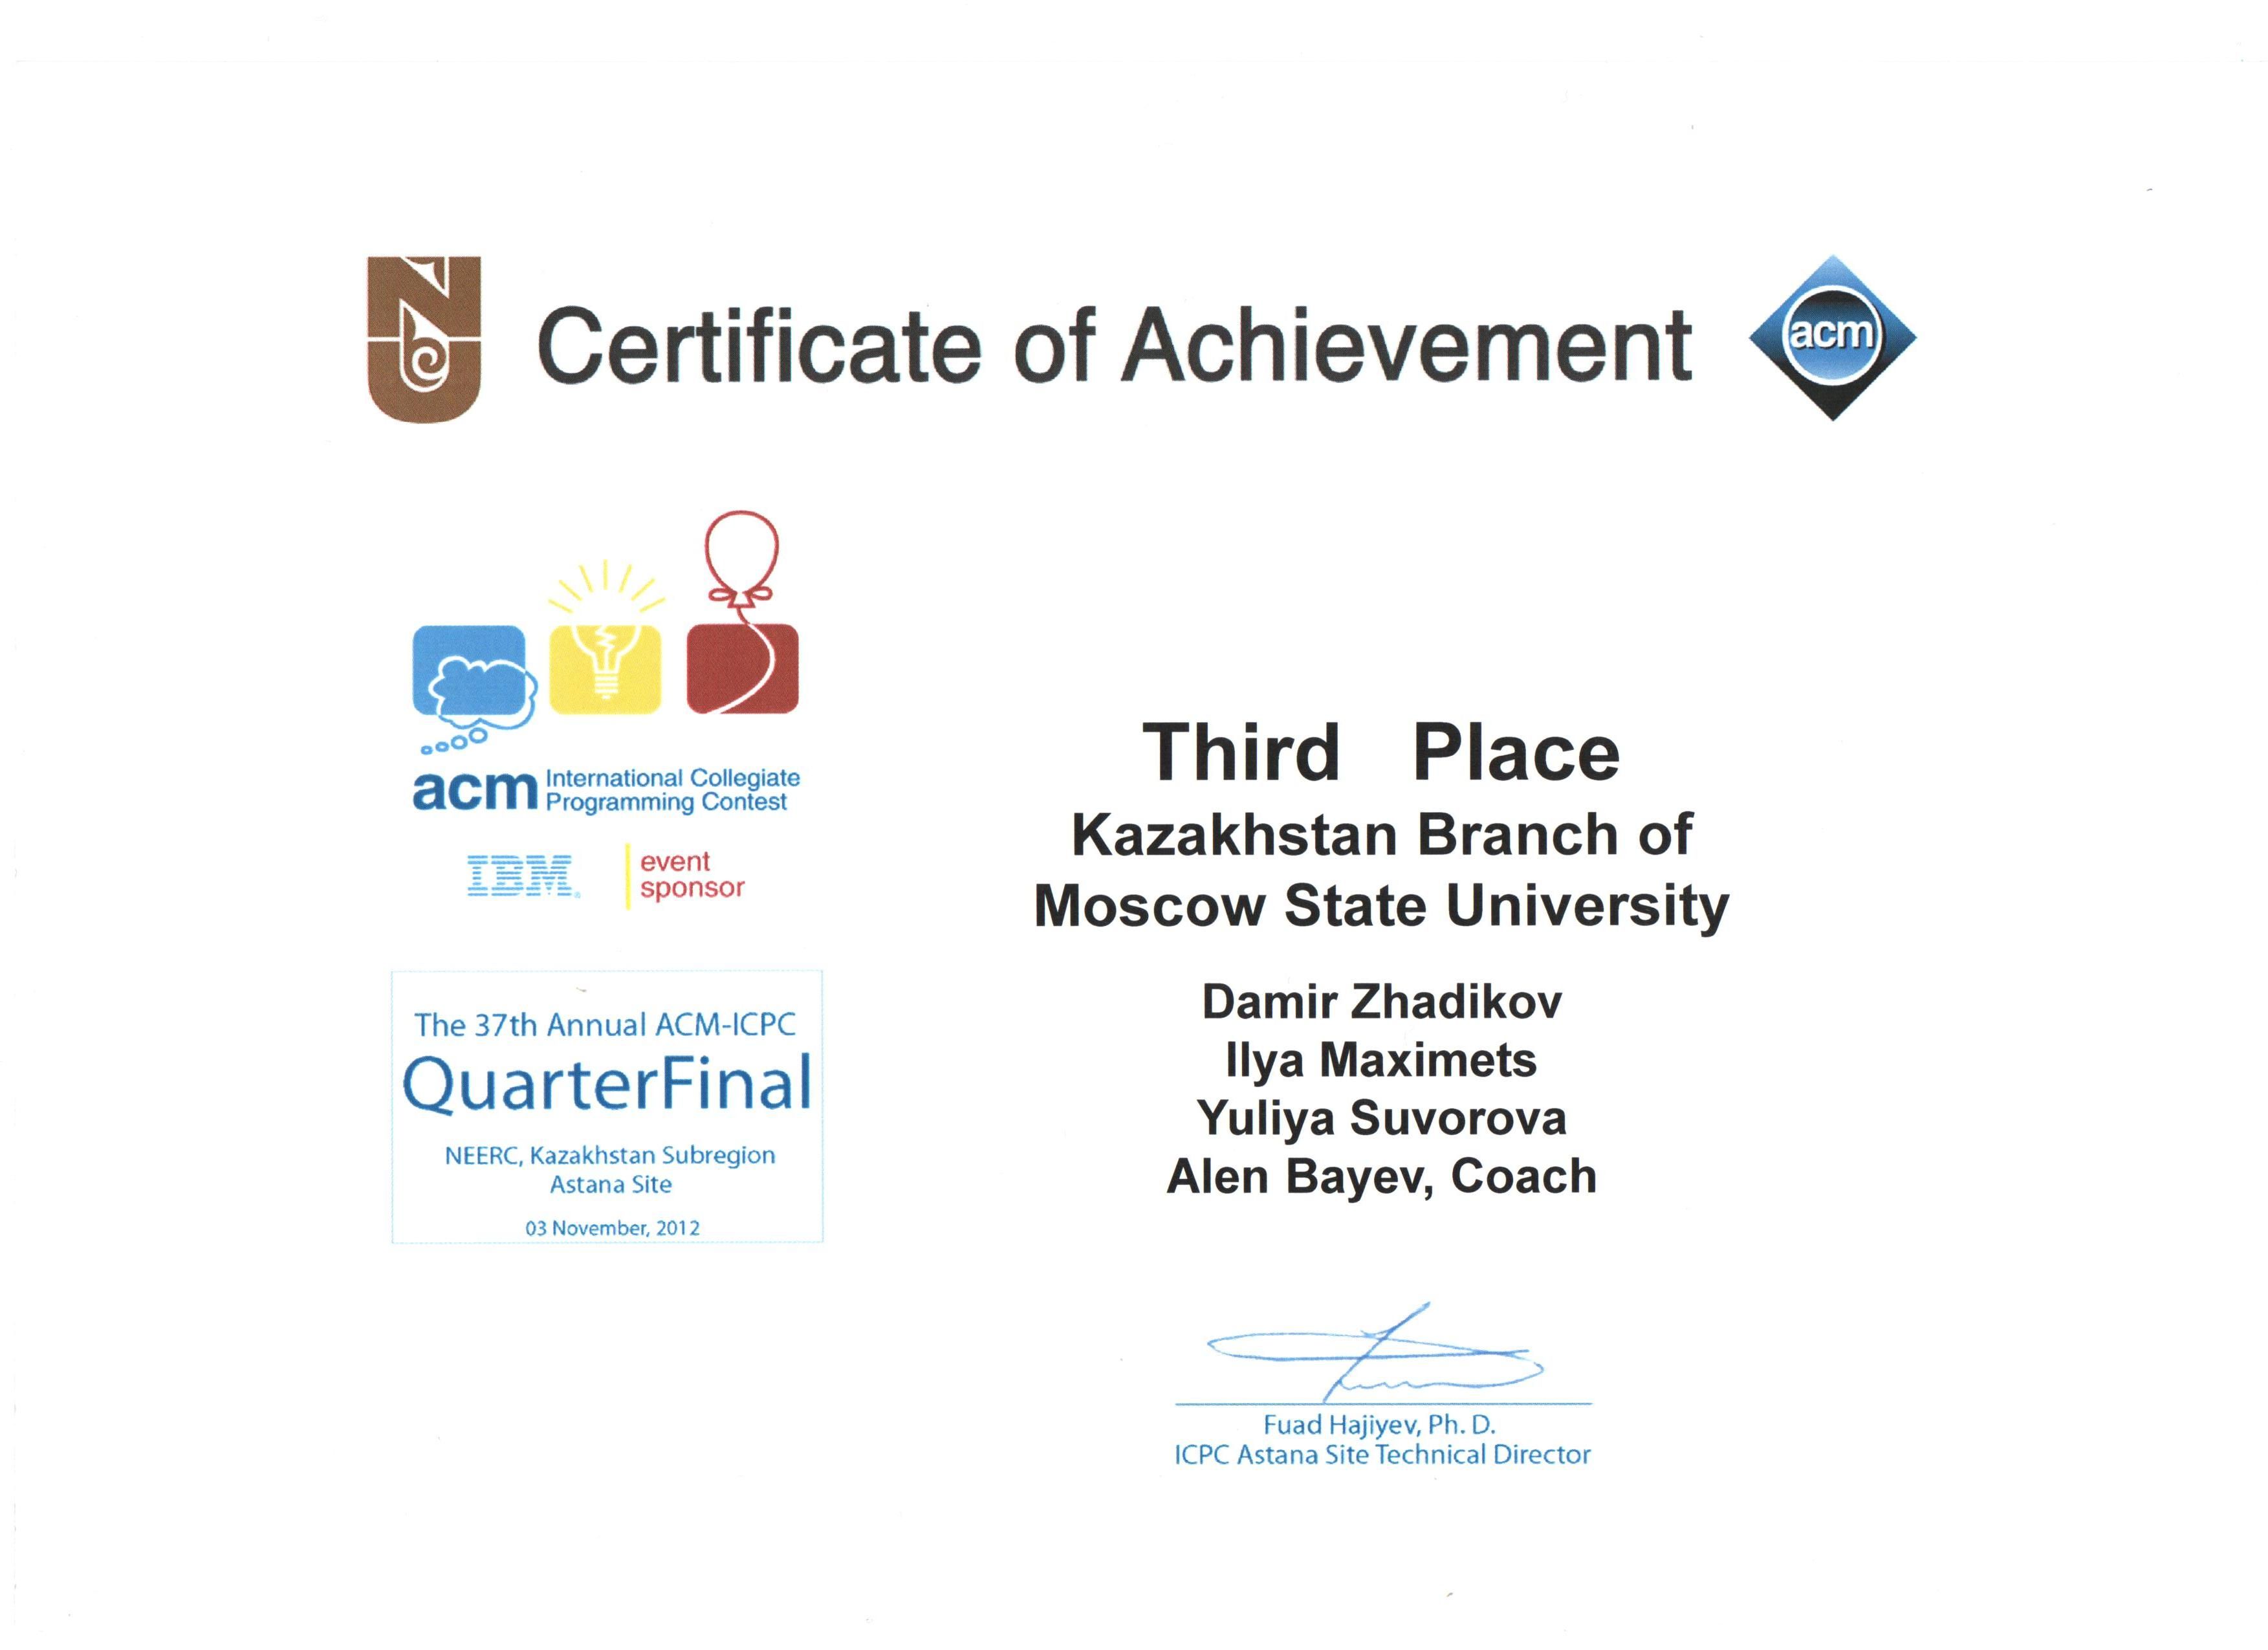
\includegraphics[width=0.7\linewidth]{diploma/2012-astana}

Диплом 3 степени среди команд Казахстана 2012\\
Команда Jusual (Максимец, Суворова, Жадиков).
\end{center}

\begin{center}
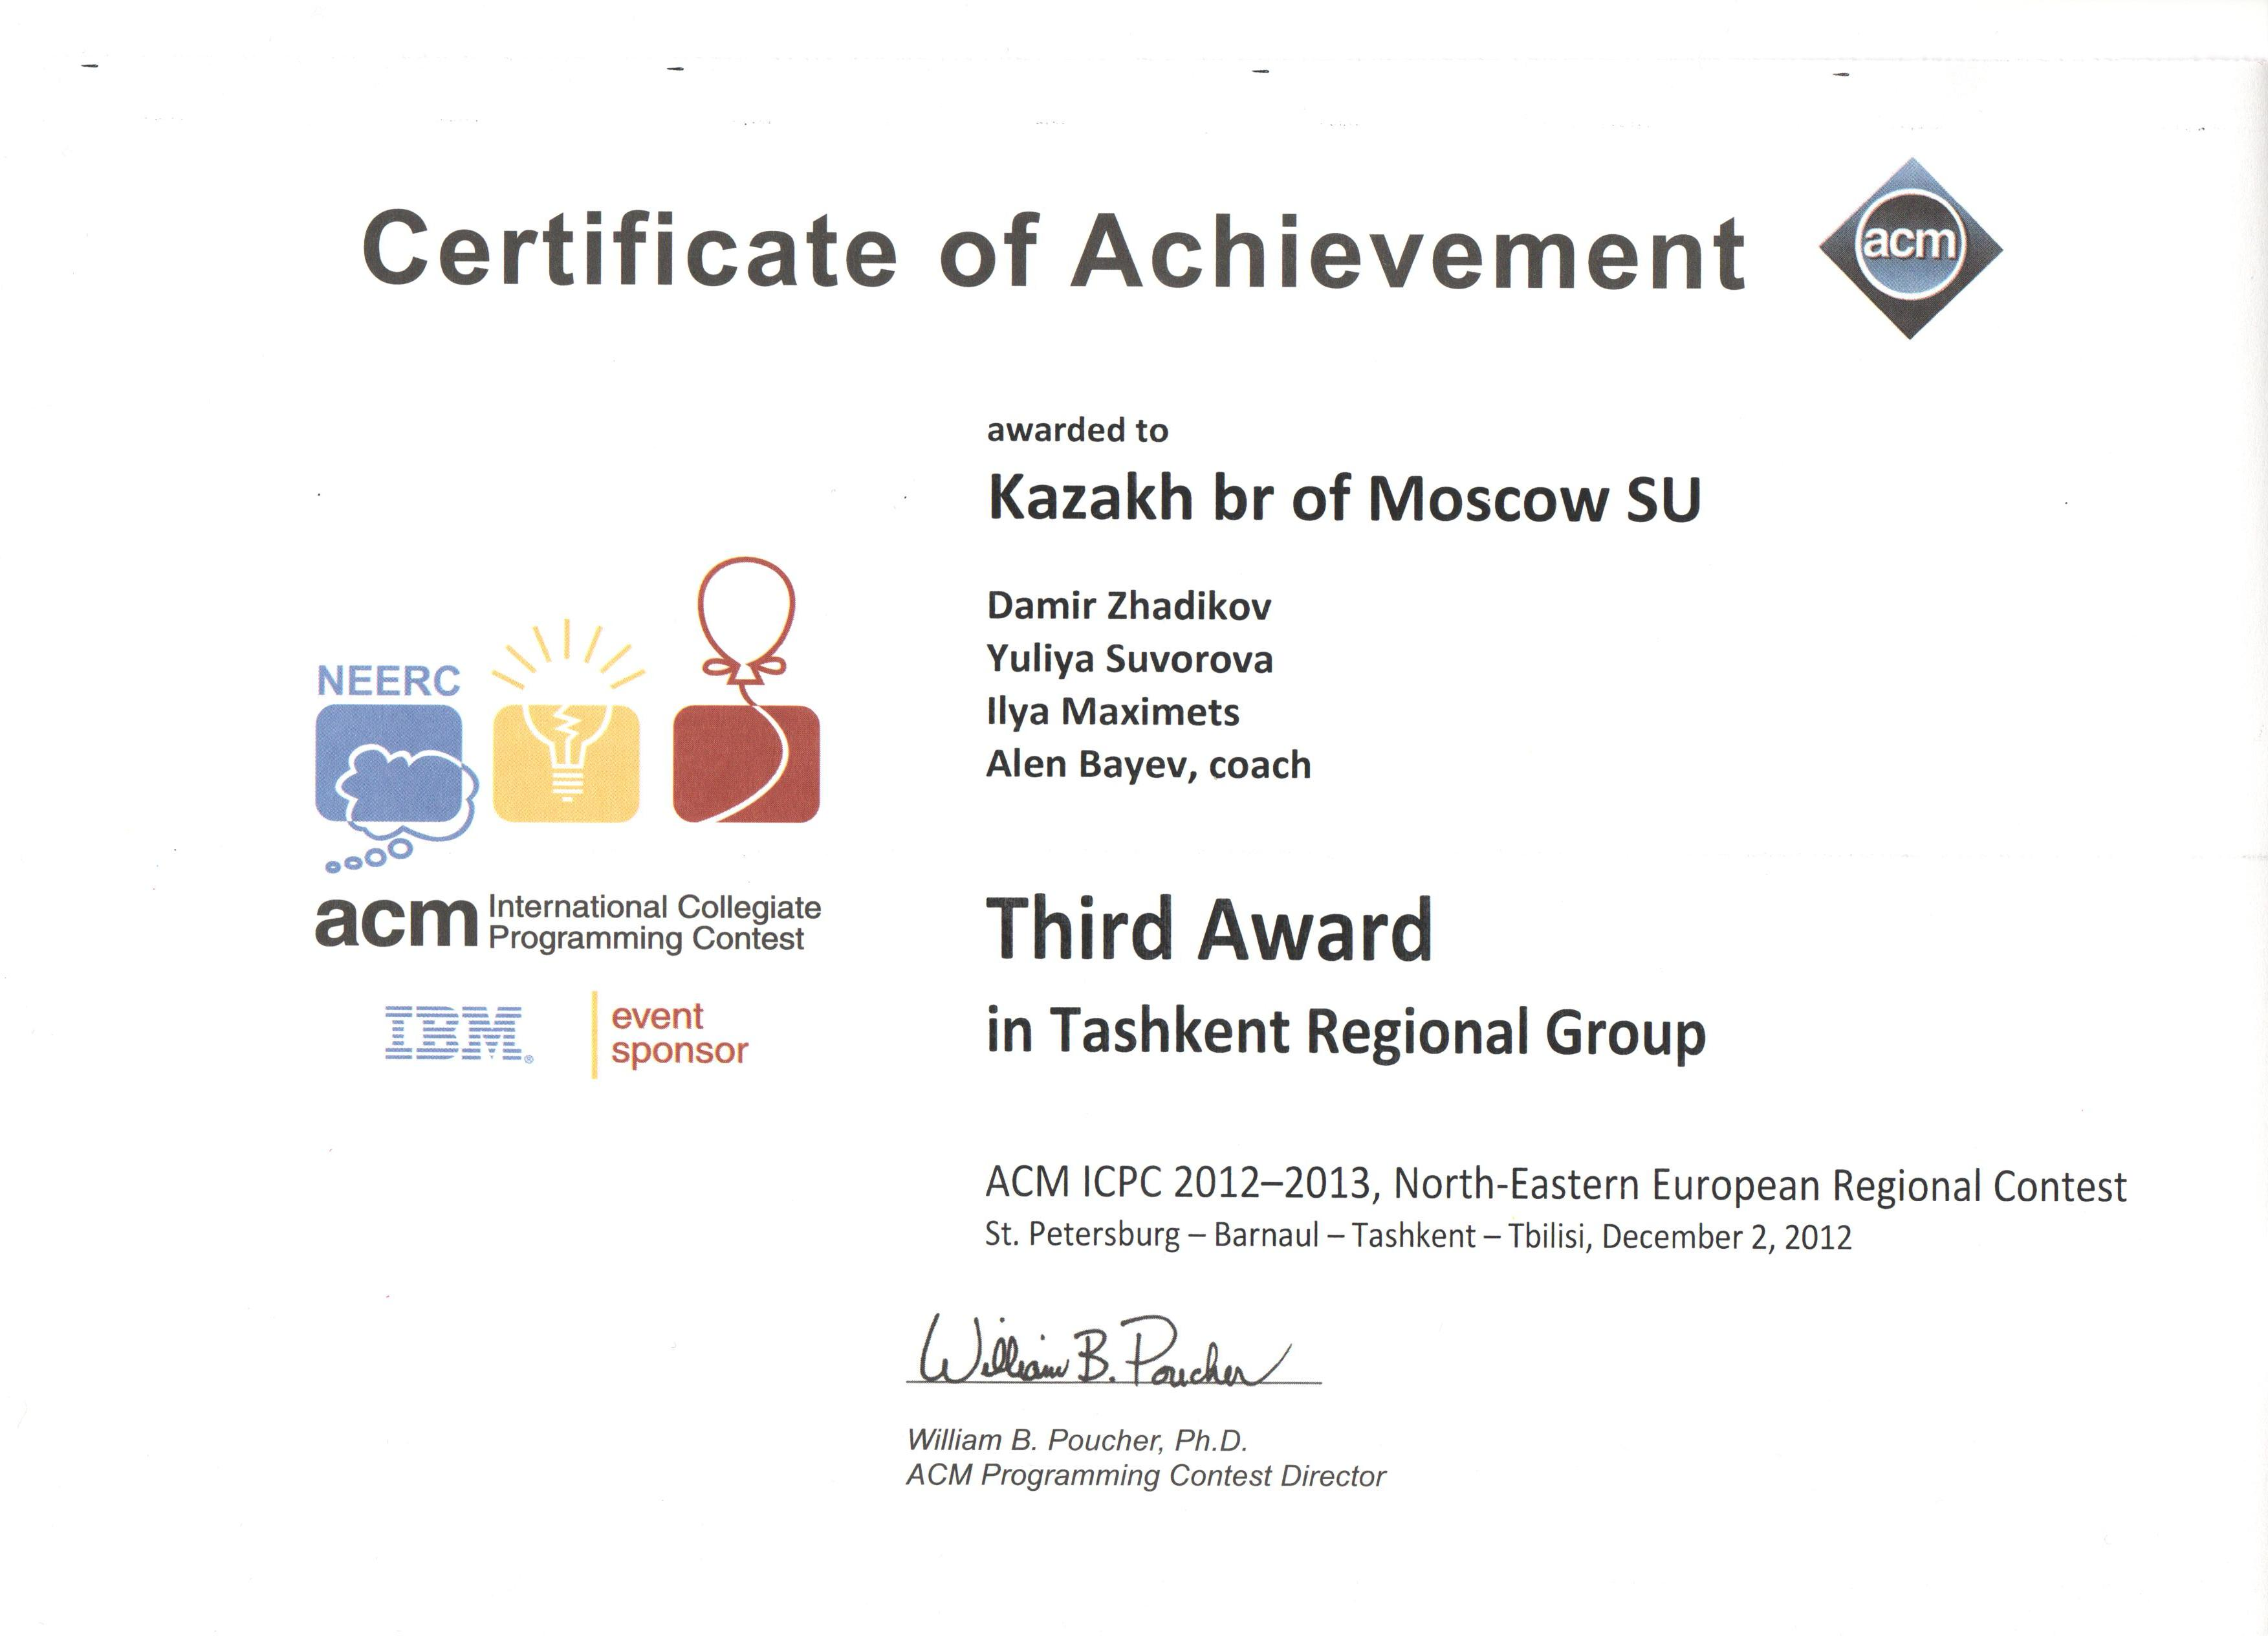
\includegraphics[width=0.7\linewidth]{diploma/2012-tashkent}

Диплом 3 степени среди команд Центральной Азии 2012\\
Команда Jusual (Максимец, Суворова, Жадиков).
\end{center}
\newpage

\subsubsection*{2013--2014 учебный год}

\paragraph{Четвертьфинал чемпионата (Казахстан).} Казахстанский филиал МГУ занял 10 место из 40 ВУЗов Казахстана, а лучшая команда филиала --- 29 место из 91 команды. Данный результат отмечен \textbf{дипломом в номинации <<Лучшая гостевая команда на площадке в Астане>>}.

\paragraph{Полуфинал чемпионата (Сибирь).} Казахстанский филиал МГУ занял 17 место из 29 ВУЗов Сибири, а лучшая команда филиала --- 25 место из 44 команд Сибири (17 место из 30 среди команд из Казахстана).

\paragraph{Полуфинал чемпионата (СНГ).} Казахстанский филиал МГУ занял 78 место из 117 ВУЗов СНГ, а лучшая команда филиала --- 147 место из 228 команд. К слову, команды МГУ заняли 2, 10, 11, 12, 27 места.

\begin{center}
\begin{tabular}{|p{1.8cm}|p{5.5cm}|p{1.5cm}|p{1.6cm}|l|}
\hline
Команда & Состав & 1/4 \newline Астана & 1/2 \newline Барнаул \\
\hline
Big dipper &
Тлеубаев Адиль, ВМ-2, \newline
Таранов Денис, ВМ-1, \newline
Шокетаева Надира, ММ-1. 
&
29 место \newline
5 задач
&
25 место \newline
2 задачи
\\
\hline
Lord \newline Bendtner \newline Team &
Седякин Илья, ВМ-1, \newline
Таскынов Ануар, ВМ-1, \newline
Васильев Андрей, ВМ-1. 
&
46 место \newline
4 задачи
&
-
\\
\hline
\end{tabular}
\end{center}

\newpage
\mbox{}
\vfill
\begin{center}
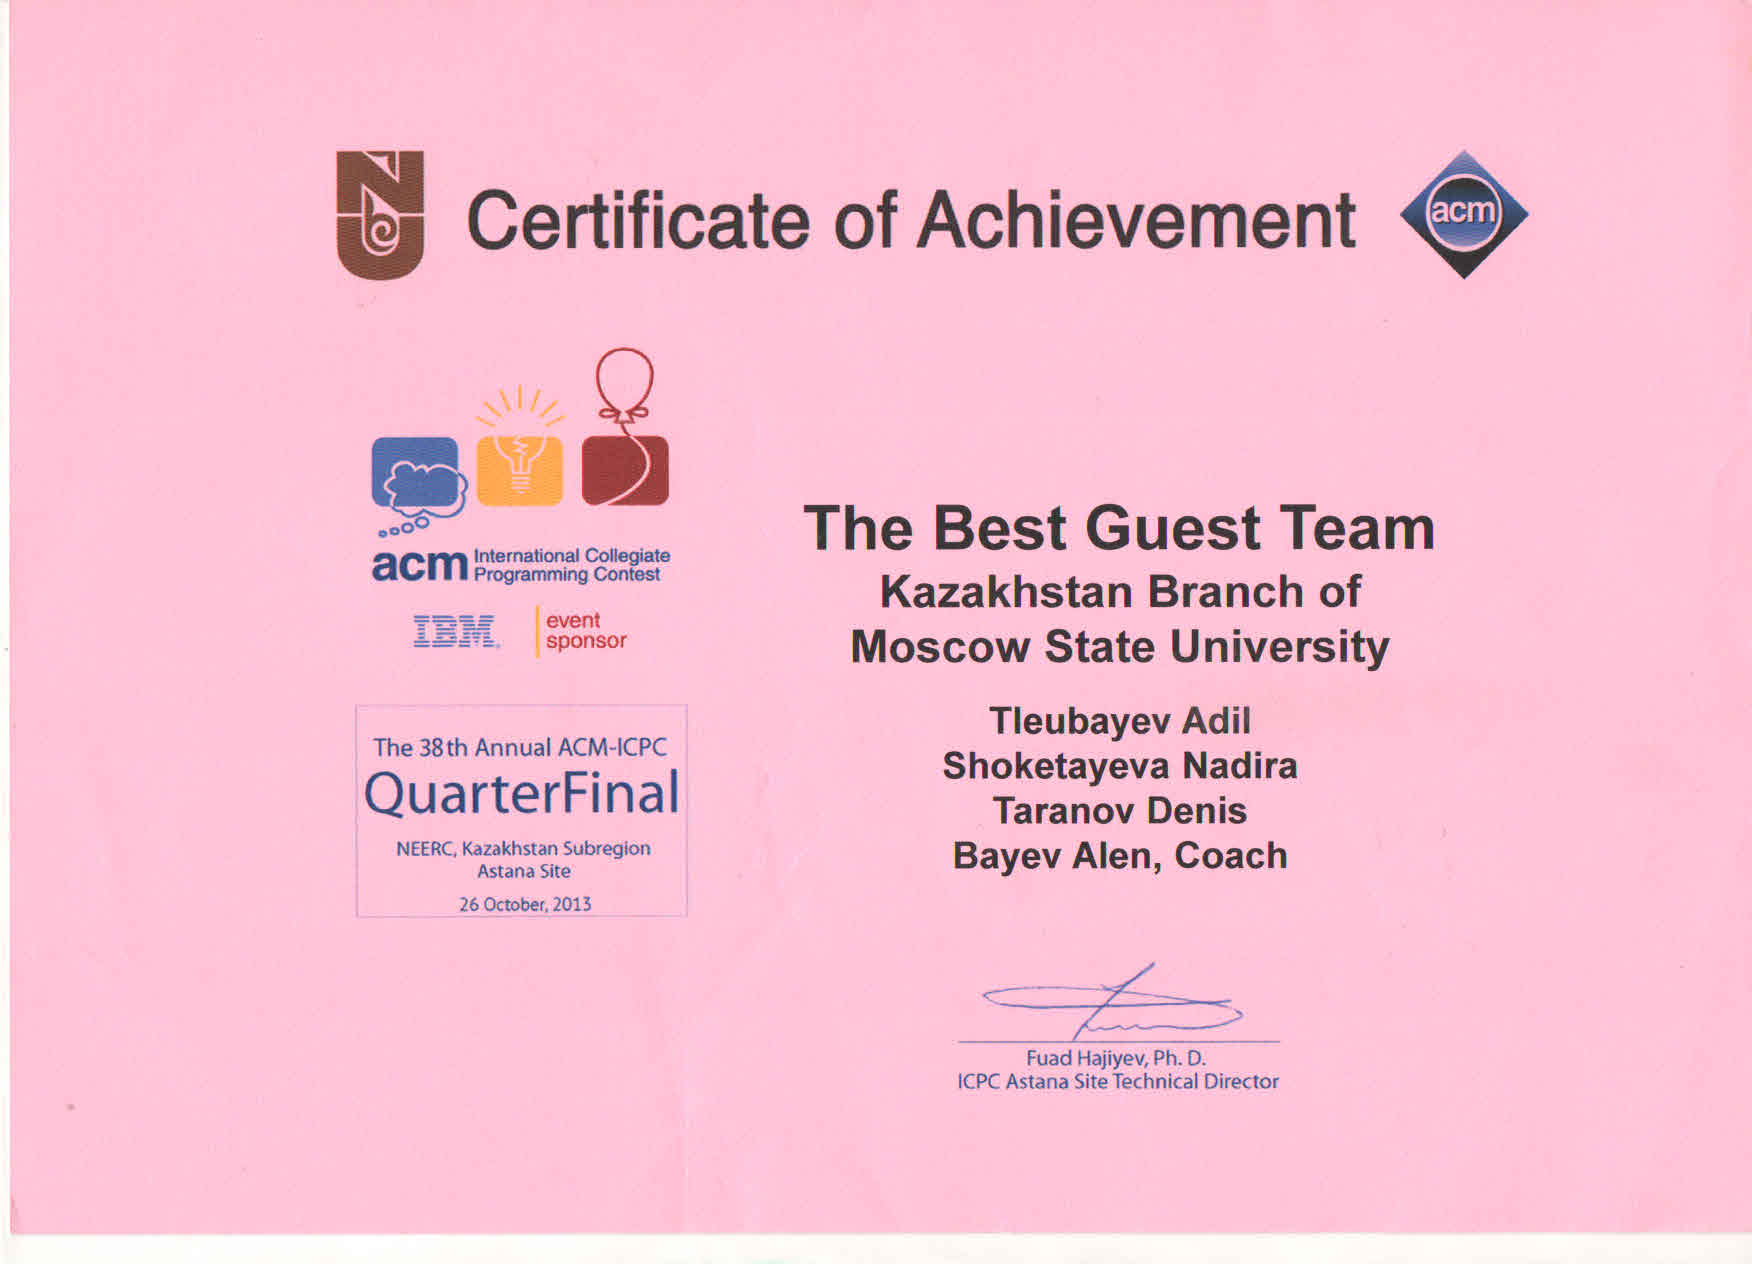
\includegraphics[width=0.8\linewidth]{diploma/2013-astana}

Диплом в номинации <<Лучшая гостевая команда на площадке в Астане>>

Команда Big dipper (Тлеубаев, Таранов, Шокетаева).
\end{center}
\vfill
\mbox{}
\newpage
\subsubsection*{2014--2015 учебный год}

\paragraph{Четвертьфинал чемпионата (Казахстан).} Казахстанский филиал МГУ занял 8 место из 30 ВУЗов Казахстана, а лучшая команда филиала --- 24 место из 98 команды.

\begin{center}
\begin{tabular}{|p{1.8cm}|p{5.5cm}|p{1.5cm}|p{1.6cm}|l|}
\hline
Команда & Состав & 1/4 \newline Астана & 1/2 \newline Барнаул\\
\hline
Lord \newline Bendtner \newline Team &
Седякин Илья, ВМ-2, \newline
Таскынов Ануар, ВМ-2, \newline
Вержбицкий Владислав, ВМ-2. 
&
24 место \newline
4 задачи
&
-
\\
\hline
MSU 4 &
Амир Мирас, ВМ-2 \newline
Шабхатов Асылжан, ВМ-2 \newline
Токтаганов Адиль, ММ-2 &
39 место \newline
3 задачи
&
-
\\
\hline
Snowy \newline Cube &
Журавская Александра, ВМ-1 \newline
Камалбеков Тимур, ВМ-1 \newline
Абайулы Ерулан, ВМ-1
&
42 место \newline
2 задачи
&
x
\\
\hline
Big \newline Dipper &
Таранов Денис, ВМ-2 \newline
Шокетаева Надира, ММ-2 \newline
Жусупов Али, ММ-1
&
44 место \newline
2 задачи
&
x
\\
\hline
\end{tabular}
\end{center}

\newpage

\subsubsection*{2015--2016 учебный год}

\paragraph{Четвертьфинал чемпионата (Казахстан).} Казахстанский филиал МГУ занял 6 место из 15 ВУЗов Казахстана, а лучшая команда филиала --- 23 место из 78 команд.

\paragraph{Полуфинал чемпионата (Сибирь).} Казахстанский филиал МГУ занял 12 место из 29 ВУЗов Сибири, а лучшая команда филиала --- 17 место из 44 команд Сибири (14 место из 16 среди команд из Казахстана).

\paragraph{Полуфинал чемпионата (СНГ).} Казахстанский филиал МГУ занял 70 место из 122 ВУЗов СНГ, а лучшая команда филиала --- 129 место из 224 команд. Данный результат отмечен дипломом третьей степени среди команд Сибири. К слову, команды МГУ заняли 4, 8, 65 и 68 места.

\begin{center}
\begin{tabular}{|p{1.8cm}|p{5.5cm}|p{1.5cm}|p{1.6cm}|l|}
\hline
Команда & Состав & 1/4 \newline Астана & 1/2 \newline Барнаул\\
\hline
Snowy \newline Cube &
Журавская Александра, ВМ-2 \newline
Камалбеков Тимур, ВМ-2 \newline
Абайулы Ерулан, ВМ-2
&
23 место \newline
6 задач
&
17 место \newline
3 задачи
\\
\hline
Big \newline Dipper &
Тлеубаев Адиль, ВМ-4, \newline
Таранов Денис, ВМ-3, \newline
Шокетаева Надира, ММ-3. 
&
25 место \newline
6 задач
&
-
\\
\hline
Lord \newline Bendtner \newline Team &
Седякин Илья, ВМ-3, \newline
Таскынов Ануар, ВМ-3, \newline
Вержбицкий Владислав, ВМ-3 
&
29 место \newline
5 задач
&
-
\\
\hline
Die \newline Perdimus &
Жусупов Али, ММ-2 \newline 
Турганбаев Сатбек, ВМ-2 \newline
Омаров Темирхан, ВМ-2
&
37 место \newline
4 задачи
&
-
\\
\hline
\end{tabular}
\end{center}

\newpage
\mbox{}
\vfill
\begin{center}
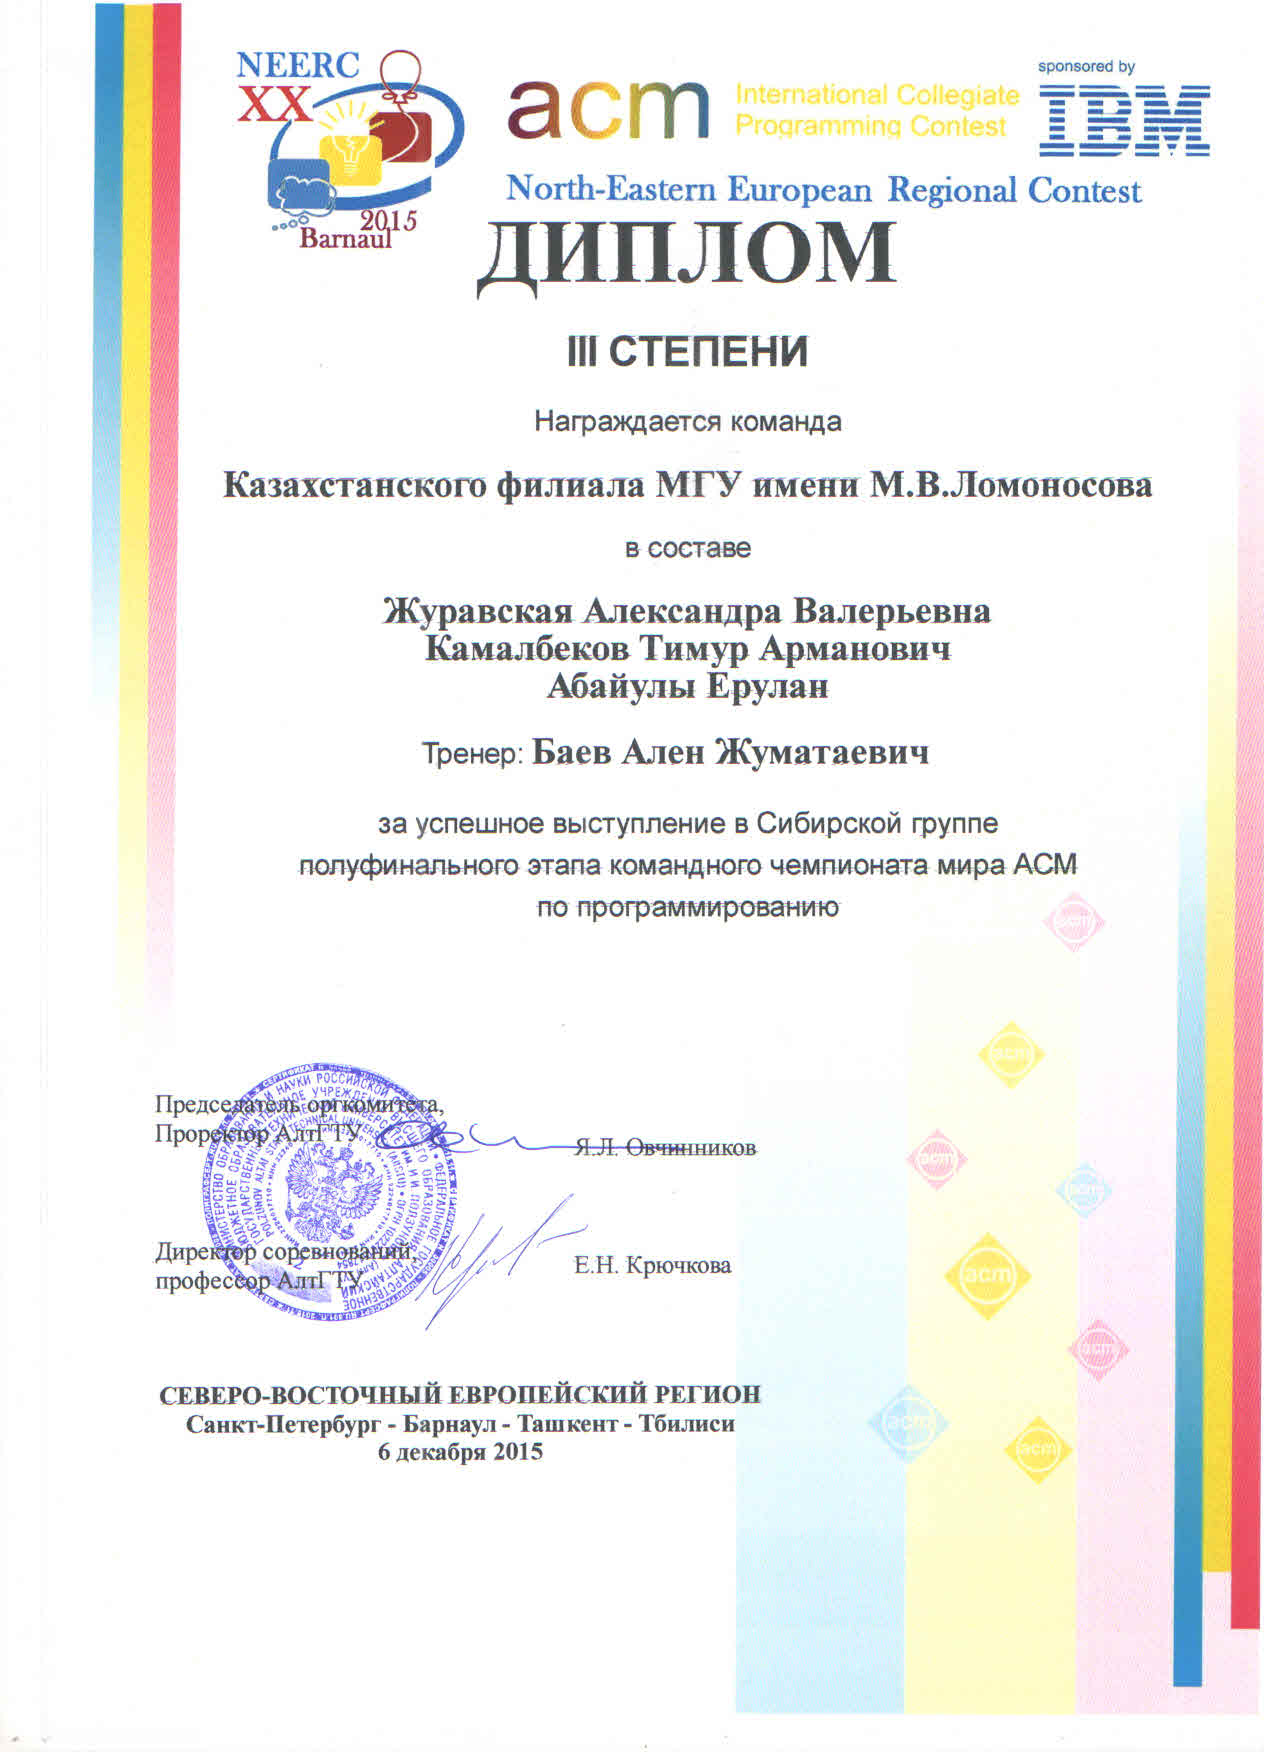
\includegraphics[width=0.8\linewidth]{diploma/2015-barnaul}

Диплом 3 степени среди команд Сибири 2015

Команда Snowy Cube (Журавская, Камалбеков, Абайулы).
\end{center}
\vfill
\mbox{}
\newpage



\subsubsection*{2016--2017 учебный год}

\paragraph{Четвертьфинал чемпионата (Казахстан).} Казахстанский филиал МГУ занял 7 место из 29 ВУЗов Казахстана, а лучшая команда филиала --- 20 место из 141 команды.

\paragraph{Полуфинал чемпионата (Средняя Азия).} Казахстанский филиал МГУ занял 5 место из 16 ВУЗов Средней Азии, а лучшая команда филиала --- 9 место из 42 команд Средней Азии (8 место из 28 среди команд из Казахстана). 

\paragraph{Полуфинал чемпионата (СНГ).} Казахстанский филиал МГУ занял 49 место из 109 ВУЗов СНГ, а лучшая команда филиала --- 93 место из 228 команд. Данный результат отмечен \textbf{дипломом третьей степени среди команд СНГ}. К слову, команды МГУ заняли 25, 27 и 72 места.

\begin{center}
\begin{tabular}{|p{2.0cm}|p{5.8cm}|p{1.5cm}|p{1.6cm}|l|}
\hline
Команда & Состав & 1/4 \newline Астана & 1/2 \newline Алматы\\
\hline
Snowy \newline Cube &
Журавская Александра, ВМ-3 \newline
Камалбеков Тимур, ВМ-3 \newline
Абайулы Ерулан, ВМ-3
&
20 место \newline
4 задачи
&
9 место \newline
3 задачи
\\
\hline
Big \newline Dipper &
Тлеубаев Адиль, ВМ-м, \newline
Амир Мирас, ВМ-4, \newline
Шокетаева Надира, ММ-4. 
&
38 место \newline
3 задачи
&
-
\\
\hline
Lord \newline Bendtner \newline Team &
Седякин Илья, ВМ-4, \newline
Таскынов Ануар, ВМ-4, \newline
Вержбицкий Владислав, ВМ-4
&
51 место \newline
3 задачи
&
-
\\
\hline
Nerzhul &
Болотников Димитрий, ММ-2 \newline
Газизов Куат, ММ-2 \newline
Аскергали Ануар, ВМ-1
&
52 место \newline
3 задачи
&
-
\\
\hline
Esprit &
Сеилов Айтмухаммед, ММ-2 \newline
Шарипов Азат, ВМ-1 \newline
Танкибаев Салима, ВМ-1
&
53 место \newline
3 задачи
&
x
\\
\hline
Complicate &
Коробов Павел, ММ-2 \newline
Бекмаганбектов Бекарыс, ММ-1 \newline
Кунакбаев Рамазан, ММ-1
&
69 место \newline
2 задачи
&
x
\\
\hline
\end{tabular}
\end{center}

\newpage
\mbox{}
\vfill
\begin{center}
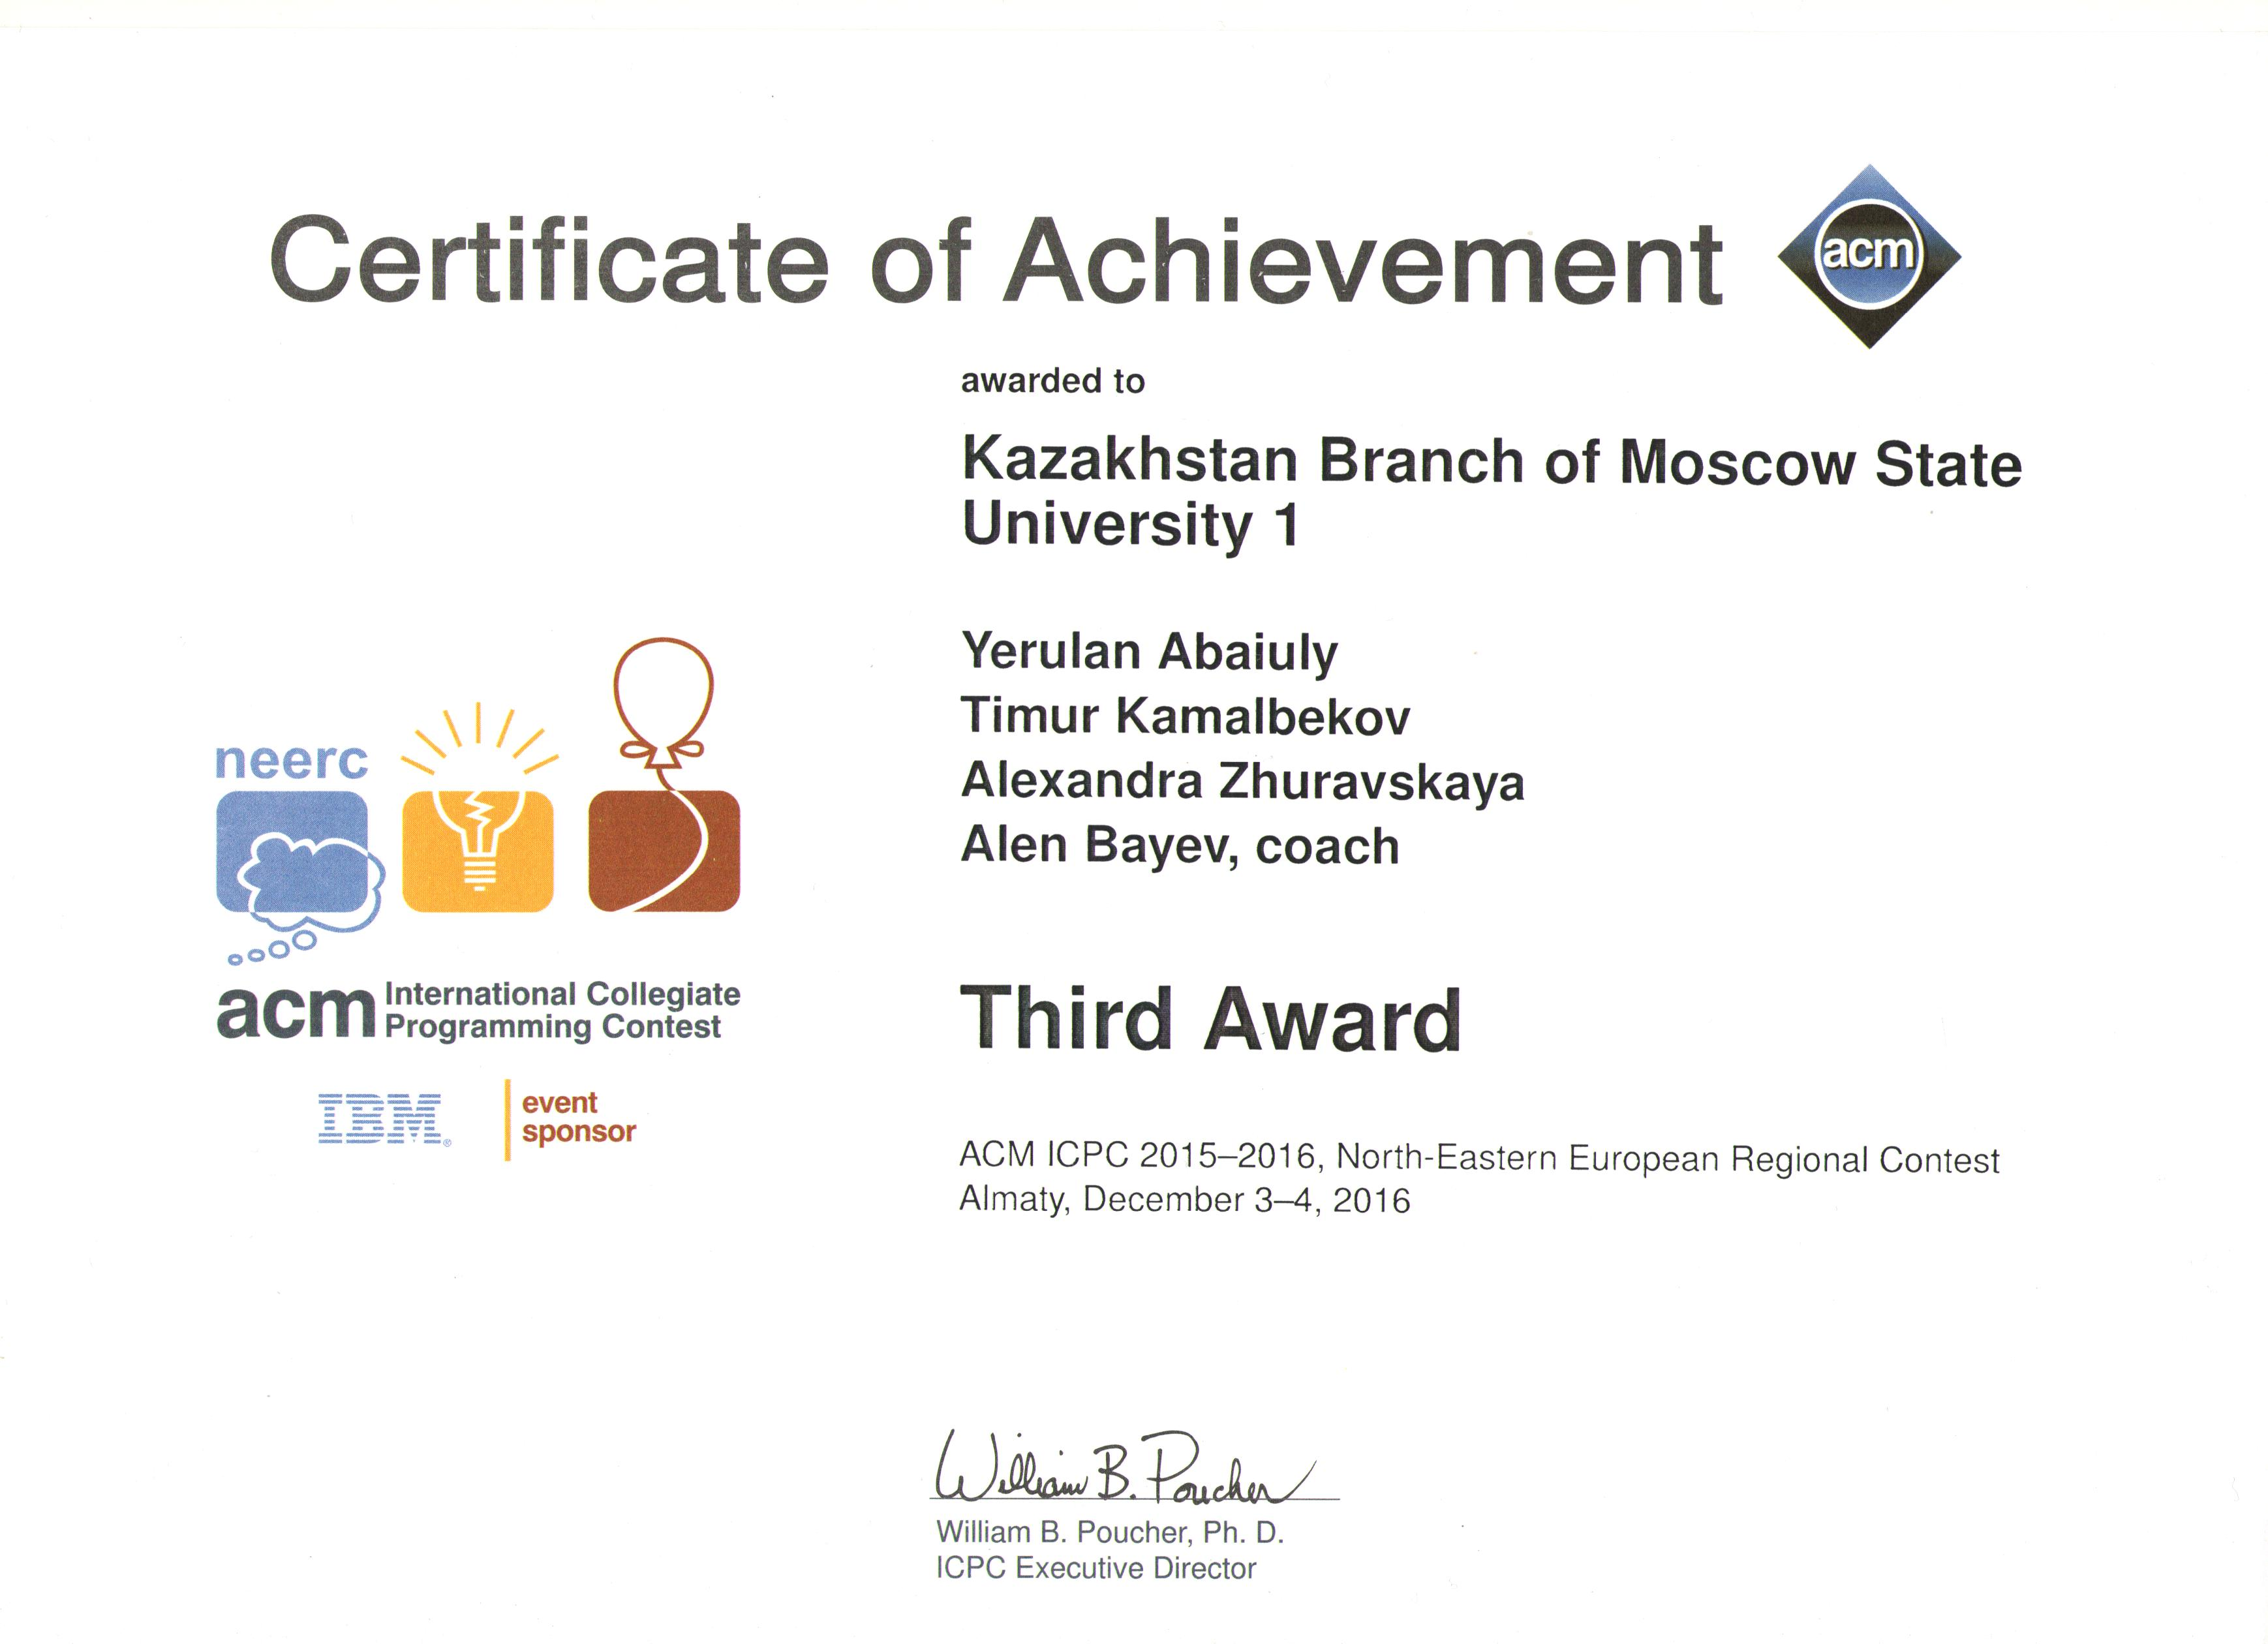
\includegraphics[width=0.9\linewidth]{diploma/2016-almaty}

Диплом 3 степени среди команд Северо-Восточного европейского региона (СНГ).

Команда Snowy Cube (Журавская, Камалбеков, Абайулы).
\end{center}
\vfill
\mbox{}
\newpage

\subsubsection*{2017--2018 учебный год}

\paragraph{Одна восьмая чемпионата (Москва).} Команда Snowy Cube участвовала в Московской ветке от МГУ. Заняла 40 место из 301 команды (11 место среди 29 команд МГУ). Данный результат отмечен \textbf{дипломом победителей одной восьмой финала в г. Москве}.

\paragraph{Четвертьфинал чемпионата (Москва).} Команда Snowy Cube заняла 48 место из 87 команды (11 место среди 12 команд МГУ).

\begin{center}
\begin{tabular}{|p{1.8cm}|p{5.8cm}|p{1.5cm}|p{1.6cm}|l|}
\hline
Команда & Состав & 1/8 \newline Москва & 1/4 \newline Москва \\
\hline
Brain \newline Burst &
Камалбеков Тимур, ВМК-4 \newline
Журавская Александра, ВМК-4 \newline
Абайулы Ерулан, ВМК-4 
&
40 место \newline
8 задач
&
48 место \newline
3 задачи
\\
\hline
\end{tabular}
\end{center}

\newpage
\mbox{}
\vfill
\begin{center}
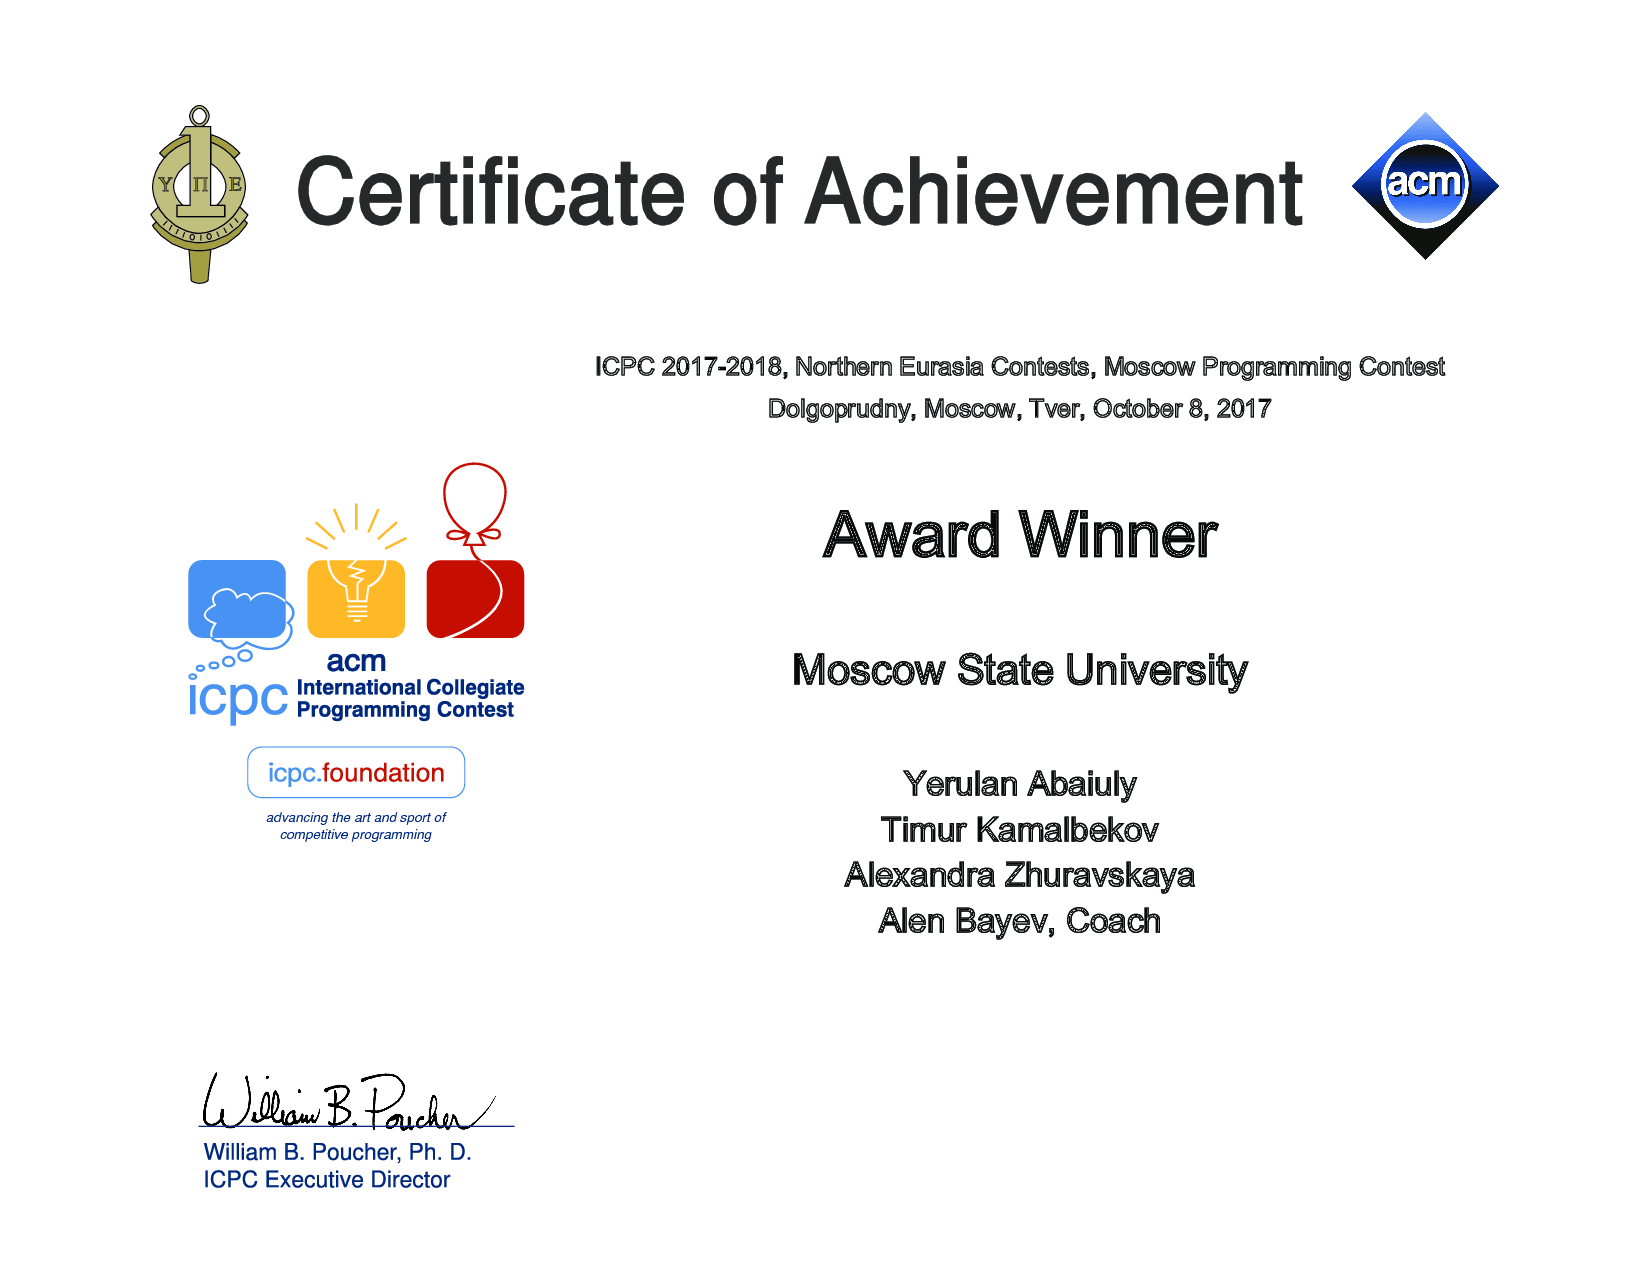
\includegraphics[width=0.9\linewidth]{diploma/2017-moscow}

Диплом победителей среди команд Москвы.

Команда Snowy Cube (Журавская, Камалбеков, Абайулы).
\end{center}
\vfill
\mbox{}
\newpage

\paragraph{Четвертьфинал чемпионата (Казахстан).} Казахстанский филиал МГУ занял 6 место из 14 ВУЗов Казахстана, а лучшая команда филиала --- 14 место из 122 команды.

\paragraph{Полуфинал чемпионата (Средняя Азия).} Казахстанский филиал МГУ занял 7 место из 45 ВУЗов Средней Азии, а лучшая команда филиала --- 10 место из 54 команд Средней Азии (6 место из 34 среди команд из Казахстана).

\paragraph{Полуфинал чемпионата (СНГ).} Казахстанский филиал МГУ занял 63 место из 126 ВУЗов СНГ, а лучшая команда филиала --- 127 место из 266 команд. К слову, команды МГУ заняли 2, 23, 30 и 40 места.

\begin{center}
\begin{tabular}{|p{2cm}|p{5.8cm}|p{1.5cm}|p{1.6cm}|l|}
\hline
Команда & Состав & 1/4 \newline Астана & 1/2 \newline Алматы\\
\hline
Brain \newline Burst &
Аскергали Ануар, ВМК-2 \newline
Бекмаганбетов Бекарыс, ММ-2 \newline
Шарипов Азат, ВМК-2 \newline
&
14 место \newline
7 задач
&
10 место \newline
3 задачи
\\
\hline
MSU 2 &
Кунакбаев Рамазан, ММ-2 \newline
Макатова Батима, ММ-2 \newline
Ержанов Жалгас, ВМК-2
&
25 место \newline
5 задач
&
-
\\
\hline
Murmaider &
Вагнер Алан, ВМК-1 \newline
Азатов Таир, ВМК-1 \newline
Понамарев Валерий, ВМК-1
&
30 место \newline
4 задачи
&
-
\\
\hline
Witty \newline name &
Газизов Куат, ММ-3 \newline
Болотников Димитрий, ММ-3 \newline
Коробов Павел, ММ-3 \newline
&
32 место \newline
4 задачи
&
-
\\
\hline
\end{tabular}
\end{center}

\newpage
\mbox{}
\vfill
\begin{center}
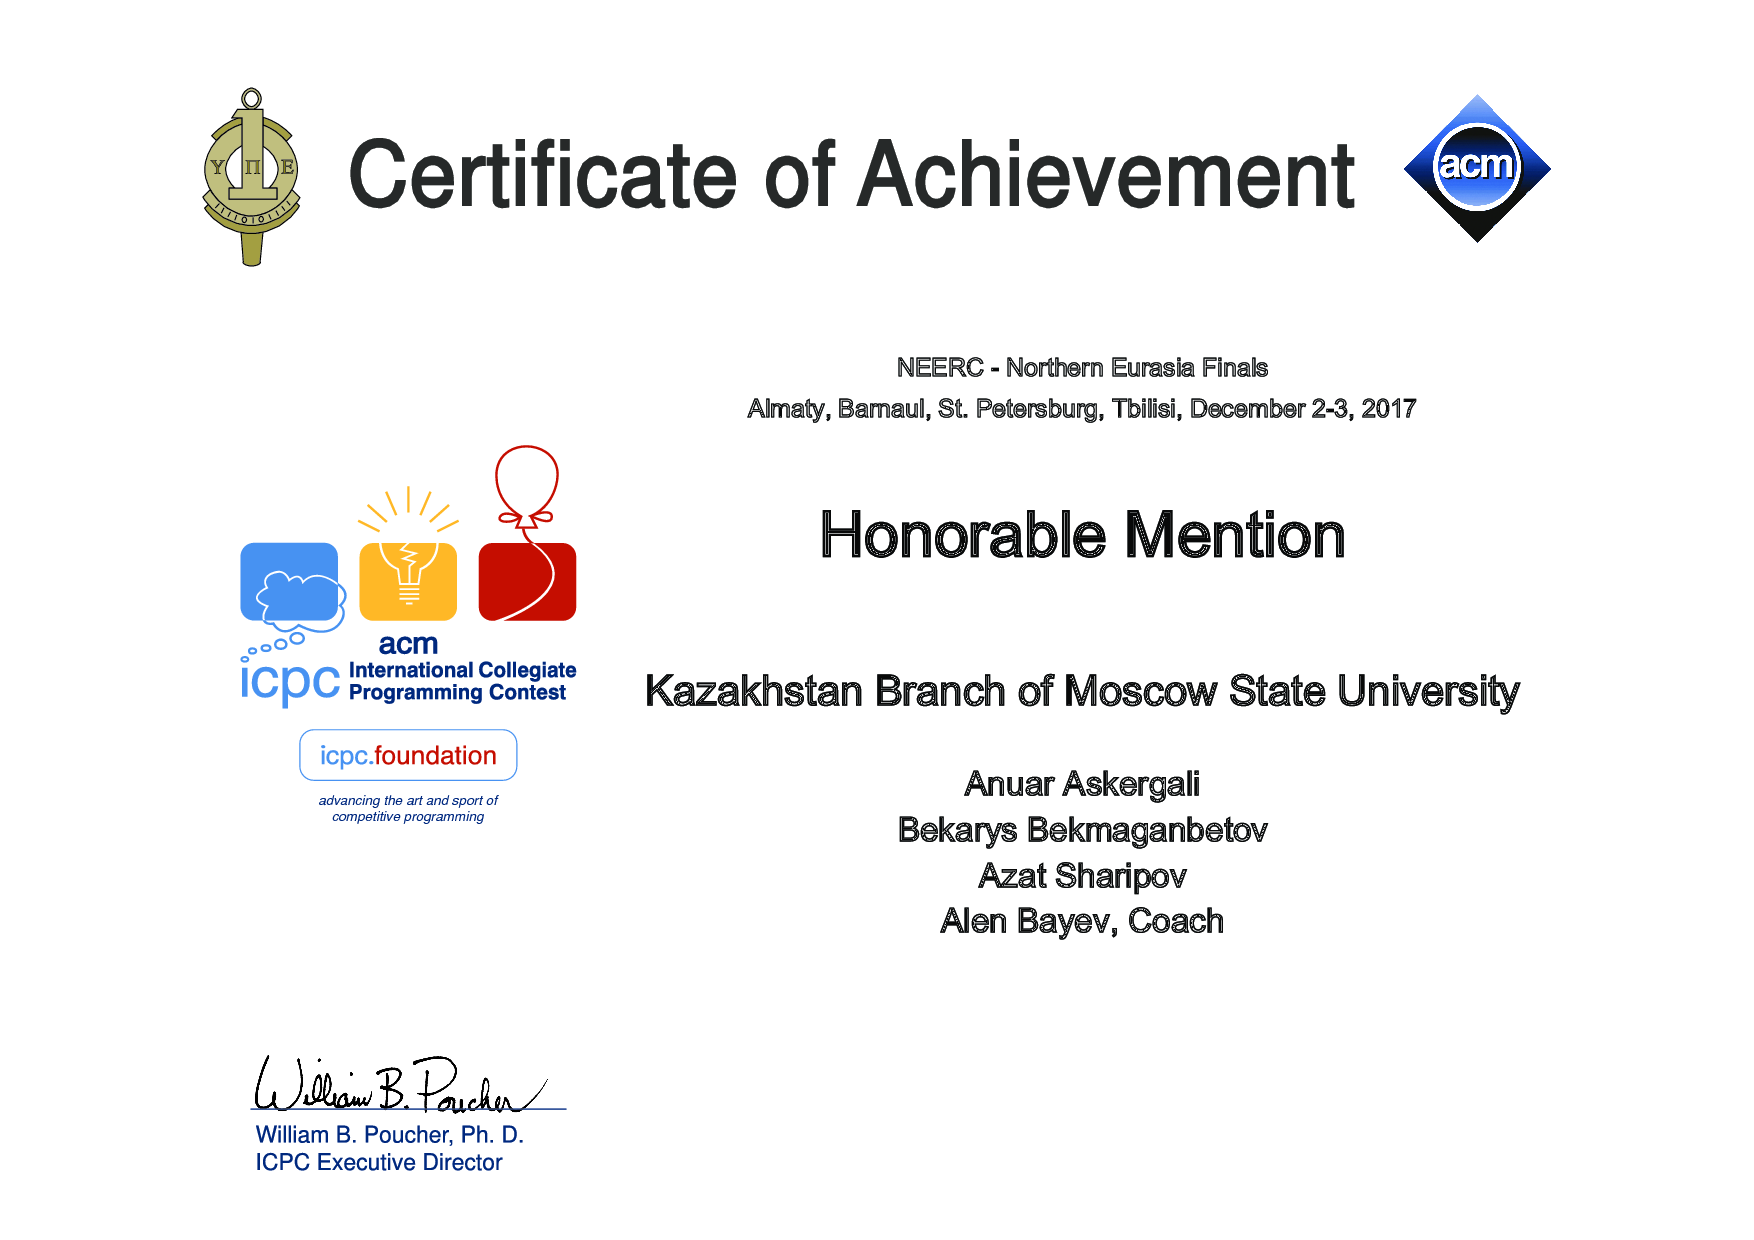
\includegraphics[width=0.9\linewidth]{diploma/2017-almaty}

Похвальная грамота среди команд Северо-Восточного европейского региона (СНГ).

Команда Brain Burst (Аскергалиев, Бекмаганбетов, Шарипов).
\end{center}
\vfill
\mbox{}
\newpage



\newpage

\section{Условия задач и результаты}

Во всех задачах до 2017 года были использованы ограничения по времени в 1 секунду, по памяти в 64 Мб. На задачи с 2018 года ограничения по времени в 1 секунду, по памяти в 512 Мб. На олимпиадах всегда гарантировалось наличие решения на языках pascal, C и С++, которые укладываются в данные ограничения. 

\makeatletter
\def\input@path{{problems/}}
\makeatother

\head{Зимний тур 2013}{11 декабря 2013}
\subsection*{A. A}

Во время разговора между Адилем и Денисом иногда звучит шутка <<A ya Denis!>>. Сколько было шуток в разговоре, если других шуток у них нет?

\informat{Строка длиной от 1 до 1000 символов, состоящая из букв английского алфавита \mbox{\tt 'a'..'z'}, \mbox{\tt 'A'..'Z'}, пробелов и 4 видов знаков препинания (,.!?). Ввод оканчивается переносом строки.}

\outformat{Одно неотрицательное число --- количество смешных шуток.}

\example{A ya Denis! A A ya Denis!}{2}

\subsection*{B. Beautiful tree}

Надира любит природу. Особенно красивые деревья. Красота дерева измеряется количеством листьев этого дерева. Посчитайте красоту дерева. 

\informat{Два натуральных числа: $n$ --- количество вершин графа (от 2 до 100), $m$ --- количество ребер графа (от 1 до $\frac{n(n-1)}{2}$). Далее $m$ пар вершин, которые соединены (вершины пронумерованы от 1 до $n$). Гарантируется, что кратных ребер и петель нет.}

\outformat{Одно натуральное число --- красоту дерева, если данный граф является деревом. Иначе выведите~0.}

\examplee
{5 4 \newline
1 3 \newline
2 5 \newline
3 4 \newline
4 2}
{2}
{6 4 \newline
1 6 \newline
2 4 \newline
4 3 \newline
6 2}
{0}

\subsection*{C. Cube}

Адиль предложил Надире и Денису загадать по одному числу от 1 до $n$ независимо друг от друга (причем каждое число с одинаковой вероятностью). Надира никогда не загадывает полные квадраты, а Денис --- полные кубы (по словам Дениса, потому что они --- <<полные>>). Какова вероятность того, что они загадают одно и то же число?

\informat{Одно целое число $n$ (от 2 до 1000).}

\outformat{Вещественное число (с точностью не менее 6 знаков после запятой) --- вероятность того, что они загадали одно и то же число. }

\examplee{3}{0.50000000}{1000}{0.00100280}

\excomm{Вероятностью случайного события $A$ называется отношение числа $n$ равновероятных элементарных событий, составляющих событие $A$, к числу всех возможных элементарных событий $N$: $P(A)= \frac{n}{N}$.}



\subsection*{D. Difficult geometry}

Адиль любит кататься на круглой лодке (радиуса $R$) в треугольном бассейне (со сторонами $a$, $b$ и $c$). Он всегда находится ровно в центре лодки. Хотя Адиль и очень хорошо плавает, он не хочет перевернуться и упасть в воду. Поэтому он плывет так, чтобы лодка всегда касалась хотя бы одной из стенок бассейна. Так Адиль хочет проплыть вдоль всего периметра бассейна. Посчитайте, какой путь проделает Адиль?

\informat{Четыре целых числа: $a$, $b$, $c$  (от 1 до 1000) --- предполагаемые размеры бассейна, $R$ --- радиус лодки (от 1 до 1000).}

\outformat {Вещественное число (с точностью не менее 6 знаков после запятой) --- длина пути, который проделает Адиль (центр лодки). Если такого бассейна нет или лодка не помещается в него, то выведите число -1.}

\exampleee{6 8 10 1}{12.00000000}{2 2 2 2}{-1}{1 2 3 1}{-1}

\excomm{Как это ни удивительно, но размерами Адиля можно пренебречь!}



\subsection*{E. Easy number}

Адиль опять предложил Надире и Денису загадать по одному числу. Но теперь числа могут быть любые целые (даже отрицательные и нули!). После этого он подсчитал <<магическое>> число --- разность квадратов загаданных чисел и сказал его Вам. Ваша задача - подсчитать сколько различных целых пар чисел $(A, B)$ могли загадать Надира и Денис (то есть сколько пар чисел дадут <<магическое>> число, равное N).

\informat{Одно целое число $N$ (от 1 до 5 000 000) --- <<магическое>> число.}

\outformat{Количество различных пар с <<магическим>> числом, равным $N$.}

\examplee{1}{2}{2}{0}



\subsection*{F. Friends}

Денис из поездки решил привезти друзьям магнитики. Он хочет подарить всем друзьям равное число магнитиков. Денис точно не помнит сколько у него друзей, но точно знает, что их не более $n$. Какое наименьшее число магнитиков ему надо купить, чтобы он при любом ненулевом количестве друзей смог раздарить все магнитики?

\informat{Одно целое число $n$ (от 1 до 22) --- максимальное возможное количество друзей.}

\outformat{Одно целое число --- минимальноe возможное количество магнитов.}

\exampleee{1}{1}{2}{2}{3}{6}



\subsection*{G. Game}

Адиль купил игру Дженга (из $N$ деревянных брусков квадратного сечения). Поскольку точных правил игры он не знает, то он придумал свои правила: двое игроков по очереди берут бруски. За ход можно взять 1 брусок, 2 бруска или половину оставшихся брусков (если осталось нечетное количество брусков, то количество округляется в меньшую сторону, например, от 7 брусков можно взять 3). Тот, кто возьмет последний брусок, считается победителем. Адиль будет ходить первый. Может ли он гарантировано обыграть Дениса при правильной игре обоих игроков?

\informat{Одно целое число $N$ (от 1 до 100 000).}

\outformat{Выведите текст 'YES' (без кавычек), если при правильной игре выиграет Адиль и 'NO' (без кавычек) --- иначе.}

\exampleee{1}{YES}{3}{NO}{4}{YES}



\subsection*{H. Hypnoses}

Надира стоит на светофоре и ждет пока загорится зеленый свет (а это случится только через $t$ секунд). Чтобы скоротать время, она следит за машинами, которые проезжают мимо нее по дороге. Некоторые машины едут по прямой слева направо, другие справа налево. Надира в начале смотрит в точку с координатами 0. Как только мимо этой точки проезжает машина, она начинает следить за этой машиной. Если мимо машины, за которой сейчас следит Надира, проезжает другая машина (в любом направлении), она переводит взгляд на нее. Так происходит до тех пор, пока не загорится зеленый свет. Выясните, где остановится взгляд Надиры, когда загорится зеленый цвет?

\informat{Два целых числа: $t$ (от 1 до 1000) --- время, через которое загорится зеленый свет, $n$ (от 1 до 1000) --- количество машин, которые есть на дороге. Далее $2n$ вещественных чисел (от -100 до 100) $x_1$, $v_1$, $x_2$, $v_2$, $\dots$, $x_n$, $v_n$ --- координаты (отличные от нуля) и скорости машин (могут быть нулевыми). Известно, что никакие три машины не бывают в одной точке одномвременно.} 

\outformat{Одно вещественное число с точностью до 2 знаков после запятой --- координата, где остановится взгляд Надиры.}

\exampleee{10 1 \newline 1 1}
{0.000000}
{10 1 \newline 8 -2}
{-12.000000}
{3 4 \newline -2 0.5 \newline -1 1 \newline 1 -0.5 \newline 3 0}
{-0.500000}

\excomm{Размерами машин пренебречь. Никакие 3 машины никогда не оказываются в одной точке (2 машины могут). Машины, которые проезжают через одну и ту же координату, не изменяют скорости друг друга. Машин, которые впервые попадутся Надире на глаза, не более одной.}

\result{2013-12}{11 декабря 2013}

\head{Весенний тур 2014}{17 марта 2014}
\subsection*{A. Ayat and the film}

Аят решил посмотреть какой-нибудь хороший фильм. Он взял пустую флешку, чтобы скопировать на нее фильм с лучшим рейтингом по версии AYAT FILM RATING. Выяснилось, что флешка не резиновая, и далеко не каждый фильм помещается на нее. Поэтому Аят решил выбрать фильм с лучшим рейтингом, который поместится на флешку. Какой фильм он из этого списка выбрал? Или Аят, взгрустнув по поводу несостоявшегося киносеанса, саботированного маленькой флешкой, пошел на пару физической культуры?

\informat{Два целых числа: $S$ --- размер флешки (от 1 до 30000) и $N$ --- количество фильмов в списке (от 1 до 100). Далее $N$ пар целых чисел: $R_i$ --- рейтинг $i$-го фильма (от 1 до 100) и $V_i$ --- размер $i$-го фильма (от 1 до 30000). Рейтинги у всех фильмов различны.}

\outformat{Целое число $K$ --- номер фильма с максимальным рейтингом, который помещается на флешке. Если Аят не смог выбрать фильм, выведите -1.}

\examplee{1000 2 \newline 100 2000 \newline 50 4700}{-1}{4000 5 \newline 100 4700 \newline 20 6200 \newline 50 1400 \newline 40 700 \newline 55 4200}{3}



\subsection*{B. Big dipper}

Команда Big-dipper --- это Денис, Адиль и Надира. Но это никак не помогает решить задачу.

\informat{Два целых числа $A$ и $B$ (оба от 1 до 1000).}

\outformat{Одно целое число.}

\exampleeee{7 2}{95}{2 2}{40}{235 152}{38783}{15 25}{0}



\subsection*{C. Comparing}

Маша и Вадим написали по строке одинаковой длины $N$ из букв латинского алфавита: $a$ и $b$. Когда они сравнили строки, выяснилось, что строки отличаются. <<Так не пойдет! Сейчас мы сделаем из них одинаковые строки!>> --- сказал тот, кто повыше, пошире и носит очки. Они решили привести обе строки к общему виду. Воодушевлённый воспоминаниями годичной давности о методах сортировки, Вадим придумал следующие правила <<приведения>>: за один ход можно переставить две соседних буквы в одной из строк, если эти буквы различны (то есть $ab \rightarrow ba$ или $ba \rightarrow ab$). <<С такими правилами ты точно не приведешь строки $aa$ и $bb$ к одинаковой!>> --- ответила та, кто пониже, стройней и с хорошим зрением. Проверьте, смогут ли ребята привести данные строки к общему виду, и если смогут, то какое минимальное количество ходов понадобится?

\informat{Целое число $N$ --- длина строк (от 1 до 100). Две строки из $N$ латинских символов $a$ и $b$.}

\outformat{Целое число $K$ --- минимальное количество ходов, необходмое для приведения к общему виду. Если строки привести нельзя, выведите -1.}

\exampleee{2 \newline aa \newline bb}{-1}{10 \newline aaaaaaaaab \newline baaaaaaaaa}{9}{6 \newline baaabb \newline abbaab}{3}



\subsection*{D. Dima's divided numbers}

Диму попросили написать программу, которая перебирает все неотрицательные числа, состоящие из не более, чем $M$ цифр. Когда ему давали задание, то ни слова не сказали про систему счисления, в которой должны быть записаны числа. Поэтому хитрый Дима выбрал двоичную систему счисления, чтобы программа работала как можно быстрее (подходящих чисел в ней всего лишь $2^M$). Как только довольный Дима доложил о выполнении задания, ему дали следующее: написать такую же программу, но чтобы она работала параллельно на кластере из $D$ компьютеров, причем каждое число должно быть получено ровно одним компьютером ровно один раз. Так как Дима в глубине души за равенство всех, всего и вся, то он решил разделить числа между компьютерами так, чтобы все компьютеры перебрали одинаковое количество чисел. Выяснилось, что далеко не для любой системы счисления можно распределить все нужные ему числа поровну между $D$ компьютерами. Тогда он решил найти минимальное основание системы счисления, для которой это можно сделать. Помогите Диме! 

\informat{Два целых числа: $M$ --- максимальное количество цифр в числе (от 1 до $10^9$) и $D$ --- количество компьютеров (от 2 до $10^9$).}

\outformat{Целое число $K$ --- минимальное основание системы счисления ($K > 1$), в которой все числа из не более, чем $M$ цифр, можно разделить поровну между $D$ компьютерами.}

\exampleee{3 1000}{10}{2 12}{6}{4 48}{6}



\subsection*{E. Elegant system}
В отличии от Димы у Вани другая позиция по выбору основания системы счисления. Он считает, что двоичная система счисления --- лучшая система счисления в мире. После курса дискретной математики это мнение настолько укрепилось, что он решил в десятичной системе счисления ввести <<двоичное округление>> для чисел из устаревшей десятичной системы счисления в передовую двоичную. Суть округления довольна проста: любое натуральное число заменяется на ближайшее, в записи которого присутствуют только цифры 0 и 1.  Напишите программу, которая <<округляет>> числа. 

\informat{Целое число $N$ (от 1 до $10^{100}$). Ввод заканчивается точкой.}

\outformat{Целое число $K$ --- число, полученное после <<двоичного округления>> без ведущих нулей. Если ближайших числа два, то округлять можно в любую сторону.}

\exampleee{5556.}{10000}{1011556.}{1011111}{101101234567890.}{101101111111111}



\subsection*{F. Fantastic chess}

Андрей и Ануар играют в игру с неадекватным ферзем на прямоугольной шахматной доске. Неадекватный ферзь может ходить вправо, вниз или вправо-вниз по диагонали на любое количество клеток (только в 3 направлениях, а не в 8, как в нормальных шахматных правилах). Хоть этот ферзь и неадекватен, но с правилами этикета знаком: он не может бить другие фигуры и ходить сквозь них. В начале игры ферзь стоит в левом верхнем углу доски. Ходить начинает Андрей. Проигрывает тот, кто не может сделать ход. Кто выиграет при оптимальной игре обоих игроков?

\informat{Целые числа $N$, $M$ --- количество строк и столбцов доски соответственно (оба числа от 1 до 100). Далее матрица $N \times M$, состоящая из символов '0' (ноль --- свободные клетки) и 'x' (икс --- клетки, занятые другими фигурами). Гарантируется, что левый верхний угол помечен свободным.}

\outformat{Строка 'Andrew' (без кавычек), если выиграет Андрей. Строка 'Anuar'  (без кавычек), если выиграет Ануар.}

\exampleee{3 6 \newline
000000 \newline
0xxx00 \newline
000000}
{Andrew}
{1 1 \newline 0}
{Anuar}
{4 4 \newline
00x0 \newline
0x00 \newline
x000 \newline
0000}
{Anuar}



\subsection*{G. Geometry}

Никто уже и не помнит, какой был праздник, но суть была в торте, который Илья принес домой. На празднике было трое друзей, и Илья в магазине выбрал торт в форме прямоугольника (его легко разделить на 4 равных части). Но, транспортируя торт из магазина домой, Илья споткнулся и торт из красивого ровного прямоугольника превратился в непонятный выпуклый четырехугольник. Все 4 вишни, что украшали торт, скатились к вершинам четырехугольника так, что в каждой вершине оказалось по одной вишне. Когда Илья принес торт домой, то перед ним встала непростая задача: как его разделить на 4 равных по площади части (это же не прямоугольник на 4 равных части делить)? Но Илья не растерялся и абстрагировался! Он провел через центр квадратного стола 2 оси параллельно краям стола (хотя бы с делением стола на 4 равных части не возникло проблем) и положил торт так, что все 4 вишни оказались в разных четвертях. Внимательно присмотревшись, Илья понял, что на торте есть такая особенная точка $M$, что если через нее провести две прямые, параллельные осям, то все 4 полученных кусочка будут в форме четырехугольников, равны по площади и на каждом будет ровно по одной вишне. Осталось найти эту точку. Помогите Илье!

\informat{8 целых чисел ($X_1$, $Y_1$, $X_2$, $Y_2$, $X_3$, $Y_3$, $X_4$, $Y_4$), которые задают 4 последовательных вершины четырехугольника. Гарантируется, что N-я вершина лежит в N-й четверти ($N=1, 2, 3, 4$). Модуль каждого числа не менее 1 и не более 100.}

\outformat{2 вещественных числа с точноcтью не менее 2 знаков после запятой --- координаты точки $M$, через которые проведены разрезы. Гарантируется, что решение существует.}

\examplee{2 3 -2 2 -1 -2 3 -1}{0.5 0.5}{1 3 -1 1 -1 -3 1 -5}{0.16 -1.0}



\subsection*{H. Ha-ha-ha}

Двумерная металлическая решетка имеет вид прямоугольника $(N-1) \times (M-1)$. В узлах решетки находятся атомы, которые пронумерованы от $(1, 1)$ --- левый верхний до $(N, M)$ --- правый нижний. У каждого атома есть некоторое число электронов, причем на решетке есть ровно один электрон--непоседа на атоме $(i_1, j_1)$ и один электрон--ускоритель $(i_2, j_2)$. Все электроны, кроме непоседы, всегда остаются на своих атомах. Каждую секунду электрон-непоседа переходит из атома $A$ на соседний по горизонтали или вертикали атом $B$, если число электронов в атоме $B$ на 1 меньше, чем в $A$ (с учетом самого электрона--непоседы). Все атомы, на которых появляется электрон $A$, он отмечает. Если электрон-непоседа добирается до атома, на котором находится электрон-ускоритель, то электрон-непоседа становится сильно--заряженным и теперь может перепрыгивать через один атом. Электрон делает прыжок из атома $A$ в атом $B$ через атом $M$, если:
\begin{enumerate}
\item $A$, $M$, $B$ лежат на прямой параллельной сторонам решетки;
\item $B$ содержит на 1 электрон меньше чем А.
\end{enumerate}
При этом атом M электрон-непоседа не отмечает. Какое наибольшее количество атомов сможет отметить электрон-непоседа?

\informat{Два целых числа $N$, $M$ --- количество строк и столбцов решетки (оба числа от 1 до 100). Матрица $N \times M$, состоящая из целых чисел $A_{ij}$, --- количество электронов на позиции $(i, j)$ (все элементы матрицы от 1 до 100).
Две пары целых чисел $(i_1, j_1)$ и $(i_2, j_2)$ --- координаты электрона--непоседы и электрона--ускорителя (номер строки от 1 до $N$, столбца от 1 до $M$).}

\outformat{Одно целое число --- наибольшее возможное количество отмеченных атомов.}

\exampleee{2 2 \newline
4 3 \newline
4 5 \newline
2 1 \newline
2 2}{1}
{3 4 \newline 
3 3 3 3 \newline
3 1 1 1 \newline
4 1 3 1 \newline        
3 1 \newline
1 4}{7}
{3 3 \newline
5 5 1 \newline
5 1 5 \newline
1 5 6 \newline
3 3 \newline
3 3}{6}
\result{2014-03}{17 марта 2014}

\head{Зимний тур 2014}{9 декабря 2014}
\subsection*{A. Automultiplicative numbers}

Вадим любит делать всё заранее. Например, к зимней сессии он подготовился ещё в сентябре. А сегодня он уже предусмотрительно хочет выбрать новогодний подарок для Маши. По мнению Вадима, лучший подарок --- это множество чисел, каждое из которых равно произведению всех своих цифр в десятичной записи. Он даже придумал специальное название для них --- <<автомультипликативные>> числа. Но Маше нравятся только числа, которые лежат в пределах от $A$ до $B$. Вадим уже понял, что найти все автомультипликативные числа из заданного интервала не так просто, если Маша выберет большой интервал. Поэтому дальновидный Вадим уже сейчас хочет знать, какое наибольшее количество различных чисел, которые понравятся Маше, он сможет подарить?

\informat{Два целых числа $A$ и $B$ ($1 \le A \le B \le 10^{18}$).}

\outformat{Одно целое число --- количество автомультипликативных чисел в диапазоне $[A, B]$.}

\example{9 11}{1}

\excomm{$9 = 9$ --- автомультипликативное; $1 \cdot 0 \ne 10$ --- не автомультипликативное; $1 \cdot 1 \ne 11$ --- не автомультипликативное.}



\subsection*{B. BNF}

Мирас пишет олимпиаду по программированию, и он уже дошёл до задачи $B$! Но продолжить ему не дают первокурсники, которые пришли к нему просить помощи с упражнением на тему <<Форма Бэкуса--Наура>> (Backus--Naur Form). Вот условие упражнения:

Дана формула, описывающая множество строк в алфавите $\{a, b, c\}$:
$$<string> ::= \{a | b\} c \{a | b\}$$
Подсчитать количество строк длины $n$ в данном множестве слов.

Мирас согласился помочь и уже объяснил условие задачи:
\begin{enumerate}
\item Запись $\{word\}$ обозначает конкатенацию (присоединение) нескольких строк $word$, то есть 
$$\{word\} = word^k,$$
где \mbox{$k = 0, 1, \dots$}. Например, $\{ab\}$ обозначает слова: пустое, \textit{\textbf{ab}}, \textit{\textbf{abab}}, \textit{\textbf{ababab}} и т.д.

\item Запись $word_1 | word_2$ обозначает альтернативу из двух вариантов: $word_1$ или $word_2$.
Например, $ab | ba$ обозначает одно из двух слов: \textit{\textbf{ab}} или \textit{\textbf{ba}}.
\end{enumerate}

В частности, заданное множество содержит строку \textit{\textbf{baacab}}. Помогите первокурсникам решить их упражнение, чтобы Мирас не отвлекался и всё-таки сдал задачу $B$!

\informat{Одно целое число $N$ --- длина строки ($1 \le N \le {10}^{18}$).}

\outformat{Одно целое число --- количество искомых строк длины $N$. Так как ответ может быть очень большим, выведите его по модулю $10^9+7$.}

\examplee{1}{1}{2}{4}

\excomm{Четыре строки из второго примера выглядят так: \textit{\textbf{ac}}, \textit{\textbf{bc}}, \textit{\textbf{ca}}, \textit{\textbf{cb}}.}



\subsection*{C. Cheer up!}

Денис решил на один день отказаться от использования всех своих электронных устройств. Не удивительно, что ему сегодня так грустно. Из всех развлечений в его опустевшей комнате остался только один игральный кубик, да и тот без надписей. Денис написал на каждой грани по одному числу от 1 до 9 и начал кидать кубик. Утешением для Дениса может послужить только выпадение его любимого числа $s$ по сумме всех бросков. Найдите вероятность того, что Денис станет чуточку веселее после $n$-го броска кубика в этот день проверки силы воли.

\informat{В первой строке шесть целых чисел $x_1$, $x_2$, $x_3$, $x_4$, $x_5$, $x_6$ --- числа на гранях кубика ($1 \le x_i \le 9$, $i = 1, \dots, 6$). Во второй строке два целых числа $n$ --- количество бросков ($1 \le n \le 100$) и $s$ --- желаемая сумма ($1 \le s \le 1000$).}

\outformat{Вероятность того, что накопленная сумма после $n$ бросков будет равна $s$ (ответ вывести с абсолютной погрешностью не более 0.001).}

\exampleee{1 1 1 1 1 1 \newline 3 3}{1.000000}{1 1 1 1 1 1 \newline 3 4}{0.000000}{1 2 3 4 5 6 \newline 2 7}{0.166667}

\excomm{Кубик в первом примере при каждом броске выдаёт единицу, поэтому сумма после трёх бросков всегда будет равна трём.}



\subsection*{D. Decks}

Ануар считает себя настоящим фокусником и поэтому всегда носит с собой несколько колод карт. Однако это не простые игральные карты: на каждой карте великого иллюзиониста написана одна строчная буква английского алфавита. Прямо сейчас Ануар показывает Андрею свой самый популярный фокус с телепатией:
\begin{enumerate}
\item Ануар записывает магическое слово на бумажке;
\item Андрей выбирает любую из колод;
\item Ануар вытаскивает некоторые карты из выбранной колоды и составляет магическое слово, которое было записано на бумажке. 
\end{enumerate}
Андрей, конечно же, в чудеса и в телепатию не верит, так что он и сам может назвать это магическое слово и разоблачить Ануара, если посмотрит на все колоды сразу. Вот только он должен учитывать, что Ануар подобрал слово максимально возможной длины для придания пущего эффекта своему фокусу.

\informat{В первой строке целое число $k$ --- количество колод ($1 \le k \le 100$). В следующих $k$ строках описания этих колод; каждое из таких описаний состоит из всех букв, содержащихся в колоде, и оканчивается точкой (в каждой колоде --- от 1 до 100 карт).}

\outformat{Cлово максимальной длины, которое можно составить из любой колоды. Если таких слов существует несколько, то вывести лексикографически минимальное (слово, которое стоит раньше по алфавиту).}

\example{3 \newline aabce. \newline abca. \newline acda.}{aac.}

\excomm{В данном примере магическое слово не может быть длиннее трёх символов; а вот из допустимых слов длины три \textbf{aac}, \textbf{aca}, \textbf{caa} лексикографически минимальным является \textbf{aac}.}

\excomm{Не забудьте поставить точку после ответа. В частности, если ответом будет являться пустая строка, Вы должны просто вывести точку.}



\subsection*{E. Ellipse}

У Асылжана есть плоская эллиптическая тарелка с полуосями $a$ и $b$ неизвестного происхождения. Недавно его посетила гениальная мысль вырезать из своей тарелки новую, в форме выпуклого $n$-угольника. Естественно, он хочет сделать это так, чтобы новая тарелка имела максимальную площадь (чтобы вмещала как можно больше еды). Найдите площадь новой тарелки Асылжана.

\informat{Три целых числа $a$, $b$, $n$, где $a$, $b$ --- полуоси старой, эллиптической тарелки, $n$ --- число вершин новой, полигональной тарелки ($1 \le a \le 100$, $1 \le b \le 100$, $3 \le n \le 10$).}

\outformat{Одно вещественное число --- площадь новой тарелки (ответ вывести с абсолютной погрешностью не более $10^{-3}$).}

\examplee{1 1 4}{2}{1 4 3}{5.1961524227}



\subsection*{F. Flip}

учадазьтишертежомопенотэон,КМВететьлукафанястичувалсидалВ.

\informat{Строка из строчных букв английского алфавита, оканчивающаяся точкой (длина строки без точки --- от 1 до 100 символов).}

\outformat{Целое неотрицательное число --- ответ на задачу.}

\examplee{toreverse.}{5}{reverse.}{1}



\subsection*{G. GOR}

Адиль, как полагается нонконформисту, отрицает существование всех известных бинарных операторов (даже $\mathbb{XOR}$!) и предпочитает пользоваться своими собственными. Среди них есть ещё не известный в широких кругах оператор $\mathbb{GOR}$, с которым он знакомит всех, кто попадается ему на глаза. Со слов автора, $z = x \ \mathbb{GOR} \ y$ действует так:
$$z_k = (x_k + y_k) \mod g, $$ 
где $p_k$ --- $k$-я справа цифра в записи числа $p$ в системе счисления с основанием $g$. Чтобы убедить весь мир в значимости придуманного им оператора, Адиль готов показать, что может за считанные секунды высчитать $\mathbb{GOR}$ всех чисел от $A$ до $B$. Вот только он оставил свою программу дома, и торжественная презентация под угрозой срыва. Вся надежда только на Вас! Вы ведь сможете спасти положение и написать эту программу?

\informat{Три целых числа $A$, $B$, $g$. $A$ и $B$ --- границы оперирования($1 \le A \le B \le 10^{18}$), $g$ --- основание системы оперирования ($2 \le g \le 10$).}

\outformat{Целое положительное число --- значение выражения: \newline $A \ \mathbb{GOR} \ (A+1) \ \mathbb{GOR} \ (A+2) \ \mathbb{GOR} \ \dots \ \mathbb{GOR} \ B$.}

\exampleee{1 4 2}{4}{4 9 3}{15}{8 11 10}{28}

\excomm{В примере 3 при $g = 10$: \newline
$8 \ \mathbb{GOR} \ 9 \ \mathbb{GOR} \ 10 \ \mathbb{GOR} \ 11 = 7 \ \mathbb{GOR} \ 10 \ \mathbb{GOR} \ 11 = 17 \ \mathbb{GOR} \ 11 = 28$.}



\subsection*{H. Holes}

Надира в своих снах часто бывала в Стране Чудес. Один раз она даже обнаружила себя в каком-то лабиринте, а если точнее, то в северо-западном углу какого-то прямоугольного лабиринта, разделённого на квадратные ячейки. Оказавшаяся рядом Гусеница объяснила, что выход из лабиринта находится в юго-восточном углу, а сама Надира для достижения этого выхода может пользоваться системой кроличьих нор. Система довольно проста: запрыгивая в один конец норы, Надира вылетает из другого конца той же норы. При этом, попадая на клетку с кроличьей норой, она не обязана туда запрыгивать и может пройти мимо. Скажите, получилось ли у Надиры дойти до выхода или она проснулась, так и не узнав, что находится за лабиринтом?

\informat{В первой строке даны два целых числа $m$, $n$ --- размеры лабиринта ($1 \le m \le 100$, $1 \le n \le 100$). В следующих $m$ строках по $n$ символов в каждой --- описание лабиринта: ‘.’ --- свободная клетка, ‘\#’ --- стена, заглавная латинская буква --- вход в кроличью нору. Гарантируется, что верхний левый и нижний правый углы свободны и что каждая заглавная латинская буква либо не встречается вовсе, либо встречается ровно два раза.}

\outformat{Строка ‘YES’ (без кавычек), если из левого верхнего угла можно дойти до нижнего правого, и ’NO’ в противном случае.}

\exampleee%
{2 3 \newline
.\#.\newline
.\#.}%
{NO}%
{4 4 \newline
.\#CD \newline
D\#.. \newline
\#\#\#\# \newline
C...}%
{YES}%
{4 4%
.\#A. \newline
A\#.. \newline
\#\#\#\# \newline
....}%
{NO}

\excomm{Во втором примере последовательность действий для достижения выхода такова: один шаг на юг, запрыгиваем в нору $D$, вылетаем с другого конца, один шаг на запад, запрыгиваем в нору C, вылетаем с другого конца, идём на восток до выхода. В третьем примере южная комната лабиринта недостижима.}



\subsection*{I. Interesting permutation}

У Ильи и Вики очень разные вкусы. Вика любит перестановки. То есть такие наборы чисел ($a_0$, $a_1$, $a_2$, $\dots$, $a_n$), которые являются перестановками чисел (0, 1, 2, $\dots$, $n$). Илья же в последнее время в восторге от полных квадратов. Поэтому набор ему интересен, только если $a_k+k$ является точным квадрат целого числа для любого $k = 0, 1, 2, \dots, n$. Набор ($a_0, a_1, a_2, \dots, a_n$), которые понравятся им обоим, Вика и Илья решили называть интересной перестановкой. Теперь они очень хотят увидеть хотя бы одну интересную перестановку для заданного $n$.

\informat{Одно целое число $n$ ($1 \le n \le 30000$).}

\outformat{Любая последовательность из ($n+1$) числа, образующая интересную перестановку. Ответ гарантировано существует.}

\examplee{3}{0 3 2 1}{2}{1 0 2}

\excomm{В первом примере: $0 + 0 = 0^2$, $3 + 1 = 2^2$, $2 + 2 = 2^2$, $1 + 3 = 2^2$.}

\result{2014-12}{9 декабря 2014}

\head{Весенний тур 2015}{18 марта 2015}
\subsection*{A. Аdamant digit}

Надира с удивлением заметила, что её новая ручка странным образом не способна писать числа, в которых есть хотя бы две различные цифры (например, 34 или 511). Надира сначала хотела расстроиться, но потом ее внезапно осенило! На самом деле осталось ещё бесконечно много натуральных чисел, которые она может выписать: 1, 2, 3, 4, 5, 6, 7, 8, 9, 11, 22, 33, $\dots$. Интересно, каково же $N$-е число в этой последовательности?

\informat{Одно целое положительное число $N$ (от 1 до $10^4$).}

\outformat{Одно целое положительное число --- $N$-е число последовательности.}

\examplee{20}{222}{100}{111111111111}


\subsection*{B. Binary palindromes}

Мирас изобрёл машину времени и теперь за символическую плату отправляет всех желающих в ближайшее прошлое. Вперёд она не работает, да и кому это нужно? Вот и сейчас к Мирасу посетитель, который хочет вернуть старые добрые деньки, когда трава была зеленее, люди --- добрее, доллар --- дешевле, а двоичная запись номера года --- палиндромом (читалась одинаково и слева направо, и справа налево). Правда, любитель поностальгировать сам не знает, какой год он имеет в виду, поэтому решать придётся Мирасу. Какой ближайший год удовлетворяет всем требованиям и нужно ли вообще отправлять этого господина в прошлое? Вдруг сейчас за окном всё то, чего просит посетитель?

\informat{Одно целое положительное число $N$ (от 1 до $10^{18}$).}

\outformat{Одно целое положительное число --- максимальный двоичный палиндром, не превосходящий $N$ (в десятичной системе счисления).}

\examplee{32}{31}{2018}{2015}

\excomm{$2015 = 11111011111_2$ --- двоичный палиндром.}



\subsection*{C. Composition of matrices}

Андрей наказан за то, что он в попытках продлить зиму залил льдом коридор университета и с радостными криками катался по нему на коньках. Теперь он не может выйти из аудитории, пока не выполнит своё задание. Задача такова: на доске выписаны некоторые операции, которые могут быть последовательно применены к некоторому двумерному вектору. Всего операций три вида: $R$ --- поворот на фиксированный угол $\alpha$, $X$ --- проецирование на ось $Ox$, $Y$ --- проецирование на ось $Oy$. Помогите Андрею и укажите минимальное целое положительное значение угла $\alpha$ в градусах, при котором существует такой вектор, что после применения к нему комбинации этих преобразований он не изменит свою длину.

\informat{Последовательность символов $R$, $X$, $Y$, оканчивающаяся символом $E$ (всего не более 1000 символов).}

\outformat{Одно целое положительное число $\alpha$ от 1 до 360 --- ответ в градусах (если ответа не существует, выведите -1).}

\examplee{XRRRXE}{60}{XRRRXRRRYE}{-1}

\excomm{В первом примере можно взять вектор $(1, 0)$. После проецирования на ось $Ox$, трёх поворотов на $60^{o}$ и повторного проецирования он сохранит свою единичную длину.}


\subsection*{D. Deep tree}

Наевшись до отвала торта, Илья решил поиграть во что-нибудь новое на своём компьютере. Его выбор пал на популярную инди--игру SuperMegaDeepTree. Её геймплей довольно прост: каждый раз, как он щёлкает по пузырьку, содержащему пару чисел $(a, b)$, на экране появляются две новых пары: $(a, a+b)$ и $(a+b, b)$. Какое минимальное число щелчков нужно сделать Илье, чтобы достичь пары $(p, q)$ и закончить игру, если в начале у него нет ничего, кроме одного пузырька с парой $(1, 1)$?

\informat{Два целых положительных числа $p$ и $q$ (от 1 до $10^{18}$).}

\outformat{Одно целое число -- минимальное число щелчков, после которого на экране появится пара $(p, q)$. Если эта цель недостижима, то вывести -1.}

\examplee{2 3}{2}{2015 2020}{-1}

\excomm{После щелчка на $(1, 1)$ появляются пары $(1, 2)$ и $(2, 1)$. В первом примере победа достигается после щелчка по $(2, 1)$, то есть всего нужно только два действия.}



\subsection*{E. Empty сornet}

Вадим хочет купить Маше мороженого и ради этого даже вышел на улицу и нашёл лавку, где это самое мороженое и продаётся. Однако продавец оказался с довольно специфичными вкусами. Чтобы заказать в его ларьке мороженого, нужно назвать ему три точки трёхмерного пространства, а с ними продавец делает следующее: он проводит три отрезка, соединяющих каждую из этих точек с началом координат $(0, 0, 0)$, оборачивает полученную конструкцию в кулёк и уже в него наливает мороженое до самых краёв. Вадим, не особо подумав, тут же назвал точки $(x_1, y_1, z_1)$, $(x_2, y_2, z_2)$ и $(x_3, y_3, z_3)$. Чуть позже он осознал, что поспешил и начал волноваться, а какой же вообще объём мороженого получит Маша?

\informat{Три строки с координатами. В $i$-й строке 3 целых числа (от -1000 до 1000): $x_i$, $y_i$, $z_i$.}

\outformat{Одно вещественное число --- максимальный объём, который можно налить (с абсолютной погрешностью не более 0.001).}

\examplee{%
1 0 1 \newline
0 1 1 \newline
0 0 2}%
{0.166667}{%
1 0 1 \newline
0 1 1 \newline
0 0 -2}%
{0}

\excomm{Сила тяжести направлена вдоль вектора $(0, 0, -1)$.}



\subsection*{F. Fantastic system}

Денис в душе бунтарь и революционер и общественные устои он принимать никак не желает. В частности, он отказывается верить в то, что в двоичной записи можно использовать только две цифры: 0 и 1. Почему бы не использовать и цифру 2? Это ведь всё-таки ДВОИЧНАЯ запись. Вот только когда он выступил со своим предложением в своей комнате в общежитии (необходимый предварительный этап перед выступлением в Парламенте), Владислав резонно заметил, что в этом случае многие числа будут иметь несколько различных видов записи. Например, число 9 можно записать не только как 1001, но и как 121 и даже как 201. На что Денис парировал: <<Чем больше, тем лучше!>> А действительно, сколько же способов записать какое-то число в этой фантастической системе счисления?

\informat{Одно целое положительное число $N$ (от 1 до $10^6$).}

\outformat{Одно целое неотрицательное число --- количество способов записать число $N$ в фантастической системе счисления.}

\examplee{9}{3}{2015}{6}



\subsection*{G. Great graph}

Саша хотела бы увидеть на доске число $b$. Но просто написать это число она не может, так как связана ограничениями, которые она сама себе зачем-то придумала. По всей видимости, так она хочет развить в себе дух студента МГУ. Ограничения заключаются в следующем. К последнему написанному числу $p$ можно приписать число $q$, только если:
\begin{enumerate}
\item $q$ не превосходит $n$;
\item $p+q$ --- простое;
\item $q$ еще не встречалось на доске.
\end{enumerate}
В начале у Саши есть только число $a$. Найдите минимальное значение $n$, при котором эта задача выполнима.

\informat{Два целых положительных числа $a$ и $b$ (от 1 до 2000).}

\outformat{Одно целое положительное число $n$ (от 1 до 2000) --- минимальный из возможных ответов и -1, если такого n нет.}

\examplee{13 1}{4}{24 3}{5}

\excomm{Цепочка в первом примере такая: 13, 4, 1; во втором: 24, 5, 2, 1, 4, 3.}

\subsection*{H. H}

Ануар отлично знает английский алфавит, но это никак не поможет ему решить задачу.

\informat{Одно целое положительное число $n$ от 1 до 10.}

\example{8}{H}



\subsection*{I. Insidious time limit}

Тимур и Ерулан, готовясь к олимпиаде, нашли старую задачу. Путь к вершине спортивного программирования нелёгок, и пока у них не всё получается, что случилось и с этой задачей. Уже который раз подряд они получают вердикт TL на 20 тесте. Может, получится у вас? Вот сама проблема: найти $a_n$, где $a_k = a_{k-2} + a_{k-3}$ для всех $k$, начиная с 3.

\informat{Две строки: \newline на первой строке одно целое число $n$ (от 0 до $10^{18}$), на второй строке три целых числа $a_0$, $a_1$, $a_2$ (от 0 до $10^{18}$).}

\outformat{Одно целое неотрицательное число $a_n$ --- ответ по модулю $10^9$.}

\examplee{3 \newline 10 11 12}{21}{0 \newline 5 11 20}{5}



\subsection*{J. Jagged sequence}

По какой-то причине Асылжан наказан. Он сам не понимает, за что. Возможно, это как-то связано с непонятными криками в коридоре, которые он слышал сквозь дрёму, пока спал на лекции. В любом случае, теперь он не может выйти из аудитории, пока не выполнит своё задание. Задача такова: на доске выписана некоторая последовательность целых чисел. Ему нужно сделать из неё возрастающую арифметическую прогрессию с разностью 1, при этом за один ход он может прибавить единицу к какому-то числу или отнять единицу от какого-то одного числа. Понятное дело, Асылжан хочет избавиться от наказания как можно быстрее. Скажите, за какое минимальное число операций он справится?

\informat{Две строки: \newline в первой строке целое положительное $n$ (от 1 до 5000), во второй --- $n$ целых чисел $a_1$, $\dots$, $a_n$ (каждое от $-10^6$ до $10^6$).}

\outformat{Одно целое неотрицательное число --- минимальное количество операций.}

\examplee{4 \newline 1 7 5 6}{5}{3 \newline -2 -1 0}{0}

\excomm{Первый пример: прибавить 2 раза единицу к первому элементу, вычесть 3 раза единицу из второго.}
\result{2015-03}{18 марта 2015}

\head{Осенний тур 2015}{20 октября 2015}
\subsection*{A. Alternative result}

Денис, заядлый футбольный болельщик команды <<Walruses United>>, очень переживал, когда не смог посмотреть и даже узнать результаты последних матчей своего любимого клуба в чемпионате. Всё, что он знает, это то, что за победу даётся 3 очка, за ничью --- 1 очко, за поражение --- 0. Выпишите для Дениса все возможные варианты суммарного количества набранных очков за $N$ игр.

\informat{Одно целое число $N$ (от $0$ до $10^4$).}

\outformat{Целые неотрицательные числа, разделенные пробелами, --- варианты суммарного количества очков в порядке строгого возрастания.}

\example{2}{0 1 2 3 4 6}

\excomm{0 очков соответствует двум поражениям, 1 очко --- поражению и ничьей, 2 очка --- двум ничьим, 3 очка --- победе и поражению, 4 очка --- победе и ничьей, 6 очков --- двум победам.}



\subsection*{B. Boolean}

Ali found in Web one interesting quote. So, Richard Burton says, that false friendship, like the ivy, decays and ruins the walls it embraces, but true friendship gives new life and animation to the object it supports. Ali doesn’t know how it can help to solve this problem, but whatever!

\informat{Одно целое положительное число N (от 1 до 25).}

\examplee{14}{true}{1}{false}



\subsection*{C. Car collection}

Надира только что получила стипендию, что, несомненно, является поводом для покупки автомобиля. Поскольку стипендия у Надиры повышенная, то она может позволить себе две машины. Зайдя в автосалон и увидев разнообразие представленных автомобилей, Надира поняла, что непременно хочет машины двух разных марок. А можете ли Вы посчитать, сколько есть у Надиры различных вариантов покупки?

\informat{В первой строке одно целое положительное число $n$ (от $1$ до $10^5$) --- количество марок машин.\\Во второй строке массив целых чисел $a_i$ (от $1$ до $10^4$) --- количество машин $i$-й марки.}

\outformat{Одно целое положительное число --- количество способов выбрать две машины различных марок.}

\example{3 	\newline 3 2 3 }{21}

\excomm{Число способов выбрать одну машину первой марки и одну машину второй марки равно 6, первой и третьей --- 9, второй и третьей --- 6. Следовательно, ответ равен 21.}



\subsection*{D. Domino}

Для расслабления после тяжёлой домашней работы Сатбек любит играть со своим набором домино, исследуя эффект, как ни странно, домино. Костяшки из его набора, в отличие от стандартных, могут иметь разные высоты. Сейчас он расставляет их на одной прямой так, что при взгляде сбоку кажется, что на прямой стоят отрезки, перпендикулярные прямой. Отрезки --- это потому что все доминошки имеют нулевую толщину, что даёт ещё одно отличие от обыкновенных доминошек. Уже приготовившись наблюдать грандиозную цепную реакцию, Сатбек вдруг решил сначала прикинуть, а какое максимальное количество костяшек он может повалить, толкнув только одну из них? Сатбек, конечно, помнит, что падение доминошки высотой $h$ на позиции $a$ направо вызывает падение в эту же сторону всех доминошек, позиции $b$ которых удовлетворяют неравенству $a < b < a + h$. Аналогично, её падение налево вызывает падение налево всех доминошек, позиции $b$ которых удовлетворяют неравенству $a - h < b < a$.

\informat{В первой строке одно целые положительное число $n$ (от $1$ до $10^5$).\\
Далее $n$ строк содержат по 2 числа, разделенных пробелом: $x_i$ (от 0 до $10^6$) --- позиция $i$-й доминошки и $h_i$ (от 1 до $10^5$) --- ее высота.}

\outformat{Одно целое число --- максимальное количество доминошек, которое можно уронить одним касанием.}

\example{%
5	 \newline
0 3	 \newline
1 1  \newline
5 1  \newline
7 7	 \newline
9 1}{3}

\excomm{Чтобы уронить три доминошки, достаточно толкнуть четвертую доминошку влево. Тогда вместе с ней упадут третья и вторая.}



\subsection*{E. Enlarged triangle}

Чтобы отпраздновать попадание в число ста тридцати шести лучших команд Москвы на четвертьфинале ACM ICPC, Илья, по традиции, купил маленький плоский треугольный тортик. Но повод действительно исключительный, а победы великого Лорда Бендтнера следует отмечать только <<датским>> тортом (то есть, тортом с площадью, равной $S$). Выяснилось, что торт не дотягивает до <<датских>> стандартов, поэтому Илья решил увеличить площадь торта. Это он может сделать путём удлинения всех сторон треугольника на одну и ту же величину. На какое число ему нужно увеличить все стороны, чтобы получить <<датский>> торт?

\informat{Четыре целых числа $a$, $b$, $c$ (от 1 до $10^4$) и $S$ (от 1 до $10^9$). Гарантируется, что треугольник со сторонами $a$, $b$, $c$ существует и его площадь менее $S$.}

\outformat{Одно вещественное число --- длина, на которую необходимо увеличить все стороны (с абсолютной погрешностью не более 0.001).}

\example{2 3 4 6}{1.0000}

\excomm{Площадь треугольника со сторонами 2+1=3, 3+1=4, 4+1=5 равна 6.}



\subsection*{F. Footprints}

Сегодня в прямоугольном лабиринте, разделённым на единичные клетки, заблудился Ерулан (Надира из своего уже выбралась). Пока Ерулан искал выход, на один листок он набросал схему лабиринта (вид сверху), а на другой стал записывать свои ходы (R – направо, L – налево, U – вверх, D – вниз). Когда он выбрался, то на радостях потерял первый листок. А сможете ли Вы восстановить минимально возможные размеры лабиринта, в котором заблудился Ерулан, если он даст Вам только второй листок? Кстати, как сказал Ерулан, вход и выход из лабиринта необязательно должны быть на краю лабиринта.

\informat{Строка из символов 'R', 'L', 'D', 'U' длиной от 1 до $10^5$. Ввод заканчивается точкой.}

\outformat{Два целых положительных числа, разделенных пробелом, --- ширина и высота лабиринта.}

\example{RRRDDLL.}{4 3}

\excomm{Лабиринт из примера:}
\begin{center}
\begin{tikzpicture}[x=30,y=30]
\fill[color=gray](0,0) rectangle (1,2);
\fill[color=gray](1,1) rectangle (3,2);
\draw[step=1] (-0.0,-0.0) grid (4.0, 3.0);

\path[->, draw, line width=2pt] (0.5, 2.5) -- (1.5, 2.5);
\path[->, draw, line width=2pt] (1.5, 2.5) -- (2.5, 2.5);
\path[->, draw, line width=2pt] (2.5, 2.5) -- (3.5, 2.5);
\path[->, draw, line width=2pt] (3.5, 2.5) -- (3.5, 1.5);
\path[->, draw, line width=2pt] (3.5, 1.5) -- (3.5, 0.5);
\path[->, draw, line width=2pt] (3.5, 0.5) -- (2.5, 0.5);
\path[->, draw, line width=2pt] (2.5, 0.5) -- (1.5, 0.5);
\end{tikzpicture}
\end{center}



\subsection*{G. Great divisors}

Темирхан недавно услышал слова британского актёра Ричарда Бёртона о том, что ненастоящая дружба подобно плющу разрушает стены, на которых держится. После этого он не на шутку задумался о том, что каждому созданию нужен настоящий друг. И даже каждому числу! И Темирхан декларировал, что настоящим другом натурального числа будет его максимальный собственный делитель (наибольший делитель, отличный от самого числа). После этого Темирхан решил собрать вместе всех настоящих друзей чисел от 2 до $n$. А какой же отличный способ устроить друзьям веселье, если их просуммировать! Вот Темирхан и нашёл эту сумму. Что же у него получилось?

\informat{Одно целое положительное число n (от 1 до 3 000 000).}

\outformat{Одно целое положительное число --- искомая сумма.}

\example{6}{8}

\excomm{$d_2 + d_3 + d_4 + d_5 + d_6 = 1 + 1 + 2 + 1 + 3 = 8$.}



\subsection*{H. Honest gifts}

Тимур не большой сторонник сладкого, и дарить он предпочитает карандаши. У него есть $a$ красных и $b$ синих карандашей, $k$ из которых он собирается оставить себе, а остальные подарить в виде подарочных наборов. Все подарочные наборы должны быть одинаковыми, то есть, состоять из одного и того же числа красных и синих карандашей. А какое максимальное число наборов он сможет составить?

\informat{Три целых положительных числа разделенных пробелом: $a$, $b$ (от 1 до $10^6$) --- количество красных и синих карандашей соответственно и $k$ (от 1 до $\min(A, B)$) --- количество карандашей, которые Тимур оставляет себе.}

\outformat{Одно целое неотрицательное число --- максимально возможное число наборов.}

\example{27 34 5}{8}

\excomm{Если оставить себе три красных и два синих карандаша, то оставшиеся карандаши можно разбить на 8 наборов по три красных и четыре синих карандаша.}



\subsection*{I. Inner subset}

Александра не большой сторонник канцелярии, и дарить она предпочитает конфеты. У Александры есть $n$ разных коробок, и она знает, что в $i$-ой коробке находится $a_i$ конфет. Она хочет сделать подарок $k$ одногруппникам, поэтому суммарное количество подаренных конфет должно делиться на $k$, но при этом ей нельзя открывать коробки --- это за неё сделают голодные до сладкого студенты. Спрашивается, сколько способов накормить своих друзей есть у Александры? Кстати, она не прочь отдать ребятам даже пустые коробки, если такие будут.

\informat{В первой строке одно целое положительно число $n$ (от 1 до 1000) --- количество коробок.\\ Во второй строке $n$ целых чисел $a_1$, …, $a_n$ (от 0 до $10^9$) разделенных пробелами, где $a_i$ --- количество конфет в $i$-й коробке.\\ В третьей строке целое положительное число $k$ (от 1 до 1000) --- количество одногруппников.}

\outformat{Одно целое неотрицательное число --- ответ на задачу по модулю $10^9 + 7$.}

\example{%
4 		\newline 
1 2 3 4 \newline
3		}{6}

\excomm{В данном случае подойдут следующие варианты: \{~\}, \{1,~2\}, \{3\}, \{1,~2,~3\}, \{2,~4\}, \{2,~3,~4\}.}

\result{2015-10}{20 октября 2015}

\head{Зимний тур 2015}{18 декабря 2015}
\subsection*{A. Alexandra and Exam}

Александра начала готовиться к экзамену. На подготовку она выделила целых 2 недели. Сначала уровень ее знаний был $X$. После недели подготовки уровень ее знаний изменился на величину $Y$. Правда она так устала во время подготовки, что не помнит, повысился или понизился ее уровень знаний (такое тоже бывает). А после второй недели подготовки уровень изменился на величину $Z$. Александра считает, что она успешно подготовилась к экзамену, если окончательный уровень ее подготовки делится на 10 (даже если уровень знаний стал отрицательный). В конце Александра решила посчитать все возможные комбинации повышений и понижений уровня знаний, которые давали бы успешную подготовку и сложила их. Чему равна эта сумма? 

\informat{Три целых числа $X$, $Y$ и $Z$ от 1 до 10000.}

\outformat{Одно целое число -- сумму уровней знаний с успешной подготовкой (если таких успешных подготовок не было, вывести 0).}

\exampleeee{11 12 13}{10}{12 13 35}{50}{10 20 30}{40}{1 2 4}{0}

\excomm{В первом примере один вариант успешной подготовки:\\
{\tt (11+12-13) = 10}.\\ 
Во втором примере два варианта успешной подготовки:\\
{\tt (12+13+35)+(12+13-35) = 50}.\\
В третьем примере четыре успешных варианта подготовки:\\ 
{\tt (10+20+30)+(10+20-30)+(10-20+30)+(10-20-30) = 40}.\\
В последнем примере нет успешных вариантов подготовки.}



\subsection*{B. Ball and Snowy Cube}

Когда команда по спортивному программированию <<Снежный куб>> собирается вместе, то обладает некоторой <<снежной>> сферой знаний. Известно, что <<снежная>> сфера знаний --- это трехмерная сфера, которая обязательно должна помещаться в <<снежный>> куб. А <<снежный>> куб --- это трехмерный куб, у которого все ребра параллельны осям, у которого одна из вершин находится в точке (0, 0, 0). Вам необходимо определить, может ли данная сфера быть <<снежной>> сферой знаний какого-нибудь <<снежного>> куба. А если может, то вывести минимальную возможную длину ребра такого куба.

\informat{Три целых числа от $-10^9$ до $10^9$ -- координаты центра сферы и одно целое число от $1$ до $10^9$ -- радиус сферы.}

\outformat{Одно целое число -- сторону <<снежного>> куба, если он существует, или 0 иначе.}

\examplee{8 6 4 2}{10}{-1 2 -3 4}{0}



\subsection*{C. Calculation of Erulan Numbers}

Ерулан недавно обнаружил ряд замечательных чисел, которые сразу же назвал в свою честь. Число Ерулана порядка $k$ -- это $k$-значное число, которое делится на все свои цифры. Помогите Ерулану построить $n$ чисел Ерулана порядка $k$.

\informat{Два целых числа $k$ от 1 до 100 и $n$ от 1 до 1000.}

\outformat{$n$ целых положительных чисел Ерулана порядка $k$ (каждое на новой строке). Если таких чисел менее $n$, вывести 0. Если ответов несколько, разрешается вывести любой.}

\examplee{2 3}{11\newline 12\newline 15}{2 15}{0}



\subsection*{D. Do Rain Dance}

Мехматянин Али создал свою мехматянскую компьютерную сеть. Сеть состоит из $N$ компьютеров, пронумерованных от 1 до $N$. Теперь ему нужно наладить связь с сетью ВМК-шников, в которой $M$ компьютеров, пронумерованных от 1 до $M$. Однако эти 2 сети устроены совсем по-разному, поэтому соединить 2 компьютера из разных сетей не так просто: сложность соединения мехматянского компьютера номер $A$ с вмк-шным компьютером номер $B$ равна ($A+B^2$) <<ударам в бубен>> (знаменитые <<танцы с бубном>>). Для каждого мехматянского компьютера общая сложность его настройки равна сумме сложностей настройки соединений со всеми вмк-шными компьютерами. Чтобы полностью настроить сеть, Али необходимо соединить каждый мехматянский компьютер с каждым вмк-шным. Помогите вычислить количество <<ударов в бубен>>, которое необходимо будет совершить Али.

\informat{Два целых числа $N$ от 1 до $2*10^5$ и $M$ от 1 до $2*10^4$ -- количество компьютеров в мехматянской и вмк-шной сети соответственно.}

\outformat{Одно целое число -- количество <<ударов в бубен>>.}

\example{2 3}{37}

\excomm{Чтобы соеденить первый мехматянский компьютер с тремя вмк-шными необходимо $(1+1^2) + (1+2^2) + (1+3^2) = 17$ <<ударов в бубен>>, а чтобы соединить второй мехматянский с тремя вмк-шными необходимо $(2+1^2) + (2+2^2) + (2+3^2) = 20$ <<ударов в бубен>>.}



\subsection*{E. ECM and Cognitive Dissonance}

Чтобы сдать практикум на ЭВМ, необходимо решить несколько заранее подготовленных задач. Как было замечено, если сначала задачи пронумеровать целыми числами от 1 до $N$ по уровню сложности, а потом перемешать, то у студентов возникает <<когнитивный диссонанс>> от порядка задач. Причем, величина <<когнитивного диссонанса>> равна количеству пар задач под номером $i$ и $j$ таких, что $i < j$ и $i$-я задача выдается после $j$-й. Тимур точно, знает, что успешно решит все задачи, только если уровень <<когнитивного диссонанса>> от порядка задач равен в точности $k$. Помогите ему найти такой порядок выдачи задач, при котором Тимур успешно решит все задачи.

\informat{Два целых числа $n$ (от 1 до $10^5$) и $k$ (от 0 до $10^{18}$) размер массива и уровень <<когнитивного диссонанса>>.}

\outformat{Перестановку из $n$ целых чисел от 1 до $n$, если она существует, в которой уровень <<когнитивного диссонанса>> равен $k$, и 0 иначе. Если ответов несколько, разрешается вывести любой.}

\exampleee{4 3}{2 3 4 1}{4 5}{4 2 3 1}{4 100}{0}



\subsection*{F. Fibonacci and Prime Number}

Недавно Али начал готовить задачу на конференцию <<Ломоносов-2016>>. Один из пунктов задачи выглядит следующим образом: 

\textit{Дано число $N$. Проверить можно ли представить его в виде суммы простого и числа Фибоначчи или нельзя.}

Помогите Али быстрее справиться с этой задачей, ведь дальше ему нужно еще решить и более сложную задачу! 

\informat{Одно целое число $N$ от 1 до $10^{12}$.}

\outformat{Вывести два целых числа (первое -- простое, второе -- число Фибоначчи). Если разложения не существует, вывести два нуля. Если ответов несколько, то вывести тот, где число Фибоначчи наибольшее.}

\examplee{24}{3 21}{17}{0 0}

\excomm{Числа Фибоначчии определяются следующим образом: $F_1 = F_2 = 1$, $F_{n+1} = F_n + F_{n-1}$ для всех $n > 1$}.



\subsection*{G. Game of Castles}

Тимур не любит играть в компьютерные игры, потому что он любит их придумывать. Недавно, он начал разрабатывать пошаговую стратегию. Вот ее правила:

\textit{
В некотором государстве есть $N$ крепостей, которые постоянно воюют друг с другом. Каждая крепость имеет несколько стен, которые ее окружают -- это уровень защиты крепости (если стен не остается, то крепость считается разрушенной). Каждый ход жители некоторой крепости A нападают на другую крепость B. При этом на следующий ход жители этих крепостей считаются уставшими, а жители всех остальных крепостей бодрыми (изначально жители всех крепостей бодрые). Во время нападения A на B у крепости B рушатся несколько стен:
\begin{itemize}
\item 2 стены, если жители крепости A -- бодрые, а крепости B -- уставшие;
\item 1 стена, если жители крепостей A и B одновременно бодрые или уставшие;
\item 0 стен, если жители A -- уставшие, а жители B -- бодрые или если крепость A была разрушена до этого хода.
\end{itemize}
}

Тимур уже написал автоматическую стратегию, которая сама сделал несколько ходов. Выведите количество стен крепости после данных ходов!

\informat{Одно целое число $N$ от 2 до 10000 -- количество крепостей. На следующей строке $N$ целых чисел $a_1$, $a_2$, ..., $a_N$ (каждое от 1 до 100000) -- количество стен у соответствующей крепости. Далее целое число $M$ от 1 до 100000 -- количество атак. На следующих $M$ строках $M$ пар чисел $A_k$ и $B_k$ (каждое от 1 до $N$, причем $A_k \neq B_k$) -- атака $A_k$ крепости на $B_k$.}

\outformat{$N$ целых неотрицательных чисел через пробел -- количество стен у соответствующей крепости после описанных выше атак.}

\example{%
4		\newline
1 5 2 3	\newline
6		\newline
1 2		\newline
3 2		\newline
4 3		\newline
3 4		\newline
1 4		\newline
1 4}%
{1 2 0 0}

\excomm{(1,~5,~2,~3) $\Rightarrow$ 1(бодрые) против 2(бодрые) $\Rightarrow$\\
(1,~4,~2,~3) $\Rightarrow$ 3(бодрые) против 2(уставшие) $\Rightarrow$\\
(1,~2,~2,~3) $\Rightarrow$ 4(бодрые) против 3(уставшие) $\Rightarrow$\\
(1,~2,~0,~3) $\Rightarrow$ 3(уставшие) против 4(уставшие) $\Rightarrow$\\
(1,~2,~0,~2) $\Rightarrow$ 1(бодрые) против 4(уставшие) $\Rightarrow$\\
(1,~2,~0,~0) $\Rightarrow$ 1(уставшие) против 4(разрушенные) $\Rightarrow$\\
(1,~2,~0,~0)}
\resultind{2015-12}{18 декабря 2015}

\head{Весенний тур 2016}{30 апреля 2016}
\subsection*{A. Alexandra’s subtractions}

Саша в совершенстве владеет мастерством сортировки чисел, поэтому для настоящего вызова ей нужна по-настоящему сложная задача. Она решила, что будет сортировать не множество чисел, а всевозможные попарные разности чисел этого множества. Например, для множества \{1, 10, 5, 7\} она получит ответ \mbox{\{-9, -6, -5, -4, -3, -2, 2, 3, 4, 5, 6, 9\}}, а для множества \{1, 2, 3\} ответом будет \mbox{\{-2, -1, -1, 1, 1, 2\}}. Задача довольно сложная, поэтому мы вас просим найти только второе максимальное число в полученном наборе.

\informat{В первой строке одно целое число $n$, где $3 \le n \le 10^5$. \newline
Во второй строке $n$ различных целых чисел $a_1$, $\dots$, $a_n$, где $1 \le a_i \le 10^6$.}

\outformat{Одно целое число --- вторая максимальная разность.}

\example{4 \newline 1 10 5 7}{6}



\subsection*{B. Book of all the words}

Денис решил выучить язык моржей. Оказалось, что алфавит моржей состоит из $n$ букв, которые совпадают с $n$ первыми буквами английского алфавита, а язык --- из всевозможных слов длины $m$. Денис настроен решительно, поэтому он даже купил словарь, в котором все слова расположены по алфавиту. Подскажите Денису $k$-ое слово в словаре, чтобы помочь ему в изучении языка.

\informat{Три целых числа $n$, $m$, $k$, где $2 \le n \le 26$, $1 \le k \le n^m \le 10^{18}$.}

\outformat{Строка из $n$ строчных латинских букв.}

\exampleee{3 5 6}{aaabc}{26 3 1739}{cow}{20 4 99431}{milk}

\excomm{В первом примере словарь будет начинаться со слов: \textit{aaaaa}, \textit{aaaab}, \textit{aaaac}, \textit{aaaba}, \textit{aaabb}, \textit{aaabc}, \textit{aaaca}, $\dots$ .}



\subsection*{C. Changing the word}

Беда! Ответ Ерулана на задачу никак не хочет сходиться с тем, что указан в конце задачника. Чтобы подогнать своё слово (а ответом является именно слово) под правильное, он может за один шаг использовать одну из трех операций:
\begin{enumerate}
\item добавить одну любую букву в начало или конец слова;
\item убрать первую или последнюю букву слова;
\item заменить каждую букву слова на симметричную ей относительно центра алфавита (то есть, \textit{'a'} на \textit{'z'}, \textit{'b'} на \textit{'y'}, $\dots$, \textit{'z'} на \textit{'a'}).
\end{enumerate}
Чтобы Ерулана мог побольше поспать, он хочет как можно быстрее справиться с этим заданием. За какое минимальное число действий он сможет привести свою строчку к правильной?

\informat{В первой строке строка из не более чем 1000 строчных латинских букв, оканчивающаяся точкой, --- ответ Ерулана. \newline 
Во второй строке правильный ответ в таком же формате.}

\outformat{Одно целое число --- минимальное число операций, за которое первую строку можно привести ко второй.}

\examplee{drop. \newline milk.}{3}{hardcore. \newline texlive.}{8}

\excomm{В первом примере один из вариантов правильной последовательности может выглядеть так: $drop \rightarrow rop \rightarrow ilk \rightarrow milk$.}



\subsection*{D. Doubtful numbers}

Али любит вводить новые термины и обозначения. Например, составные числа, имеющие больше простых делителей, чем составных, он решил называть сомнительными. Скажите, сколько сомнительных чисел найдёт Али среди всех целых чисел отрезка $[A, B]$?

\informat{Два целых числа $A$, $B$, где $1 \le A \le B \le 10^7$.}

\outformat{Одно целое число --- количество сомнительных чисел на отрезке $[A, B]$.}

\examplee{90 100}{4}{1 2016}{564}

\excomm{Число 90 не является сомнительным, поскольку имеет 3 простых делителя (2, 3 и 5) и 8 составных (6, 9, 10, 15, 18, 30, 45 и 90); число 91 же сомнительное, поскольку имеет 2 простых делителя (7 и 13) и только 1 составной (91). Другими сомнительными числами из первого примера будут 93, 94 и 95. Число 97 также имеет больше простых делителей, чем составных, но оно само является простым.}



\subsection*{E. Experiment with tea}

У Тимура есть стакан с квадратным основанием, в котором он выложил сахар-рафинад в аккуратные столбики. На дне стакана осталось место только под один кубик сахара. Чтобы сахар быстро не растворялся, он льет чай в именно в этот свободный квадрат. Какой максимальный объем чая он может налить в стакан так, чтобы чай не касался стенок стакана?

\setsepchar{\\/ }
\readlist\levelA{%
1 1 1 1 1 1 1\\%
1 1 1 1 1 1 1\\%
1 1 1 1 1 1 1\\%
1 1 1 0 1 1 1\\%
1 1 1 1 1 1 1\\%
1 1 1 1 1 1 1\\%
1 1 1 1 1 1 1\\%
}
\readlist\levelB{%
1 1 1 1 1 0 0\\%
1 0 0 0 1 0 0\\%
1 0 1 1 1 1 1\\%
1 0 1 0 1 0 1\\%
1 0 1 1 1 0 1\\%
1 0 0 0 0 0 1\\%
1 1 1 1 1 1 1\\%
}
\readlist\levelC{%
1 1 1 1 1 0 0\\%
1 2 2 2 1 0 0\\%
1 2 2 2 1 1 1\\%
1 2 2 2 2 2 1\\%
1 2 2 2 2 2 1\\%
1 2 2 2 2 2 1\\%
1 1 1 1 1 1 1\\%
}
\readlist\levelD{%
1 1 1 1 1 0 0\\%
1 0 0 0 0 0 0\\%
1 0 0 0 1 0 1\\%
1 0 0 0 0 0 1\\%
1 0 0 0 0 0 1\\%
1 0 0 0 0 0 1\\%
1 1 1 1 1 1 1\\%
}

\newcommand{\cubeshift}[3]{ 
\coordinate (O) at (0, 0);
\coordinate (R) at (3, 1);
\coordinate (L) at (-1, 3);
\coordinate (D) at (0, -1.5);
\coordinate (Shift) at ($-#1*(R)-#2*(L)-#3*(D)$);
}

\newcommand{\cube}{ 
\begin{scope}
\draw[fill=black!60!white]
	($(O) + (Shift)$) -- 
	($(R) + (Shift)$) -- 
	($(R) + (D) + (Shift)$) -- 
	($(D) + (Shift)$) -- 
	cycle;
\draw[fill=black!60!white]
	($(O) + (Shift)$) -- 
	($(L) + (Shift)$) -- 
	($(L) + (D) + (Shift)$) -- 
	($(D) + (Shift)$) -- 
	cycle;
\draw[fill=black!30!white]
	($(O) + (Shift)$) -- 
	($(L) + (Shift)$) -- 
	($(L) + (R) + (Shift)$) -- 
	($(R) + (Shift)$) -- 
	cycle;
\end{scope}
}

\newcommand{\plane}{ 
\begin{scope}
\fill[opacity=0.7]
	($(O) + (Shift)$) -- 
	($(L) + (Shift)$) -- 
	($(L) + (R) + (Shift)$) -- 
	($(R) + (Shift)$) -- 
	cycle;
\end{scope}
}
\newcommand{\layout}[3]{
	\def\showwater{#3}
	\foreach \x in {1, ..., 7} {
		\foreach \y in {1, ..., 7} {
			\def\iscube{#1[\y,8 - \x]}
			\ifnum\iscube=1
				\cubeshift{\x}{\y}{#2}
				\cube
			\fi
			\ifnum\showwater=1
				\ifnum\iscube=2
					\cubeshift{\x}{\y}{#2}
					\plane
				\fi
			\fi
		}
	}
}

\begin{center}
\resizebox{0.45\linewidth}{!}{
\begin{tikzpicture}
\layout{\levelA}{1}{0}
\layout{\levelB}{2}{0}
\layout{\levelC}{3}{0}
\layout{\levelD}{4}{0}
\end{tikzpicture}
}
\resizebox{0.45\linewidth}{!}{
\begin{tikzpicture}
\layout{\levelA}{1}{0}
\layout{\levelB}{2}{0}
\layout{\levelC}{3}{1}
\layout{\levelD}{4}{0}
\end{tikzpicture}
}
\end{center}


\informat{В первой строке одно целое число $N$ от 1 до 100 --- сторона квадратного основания стакана, выраженная в кубиках сахара. \newline
В следующих $N$ строках ---  матрица $A$ размера $N \times N$ из целых чисел от 0 до $10^6$, где $a_{ij}$ --- высота соответствующего столбца. Гарантируется, что в матрице присутствует ровно один нулевой элемент, причем он не находится на границе матрицы.}

\outformat{Два целых числа: $h$ --- уровень чая в стакане в кубиках (при максимальном объеме) и $v$ --- максимальный объем налитого чая.}

\examplee{7 \newline
4 4 4 4 4 4 4  \newline
4 1 1 1 1 1 4  \newline
4 1 2 2 2 1 4  \newline
4 1 2 0 2 1 4  \newline
4 3 4 2 2 1 4  \newline
1 1 3 1 1 1 4  \newline
1 1 4 4 4 4 4}{3 36}
{3 \newline
2 3 4 \newline
9 0 5 \newline
8 7 6}{3 3}

\excomm{Сахар не тает и не пропускает чай.}



\subsection*{F. Five words}

\noindent
Коровы понимают каждое сказанное человеком слово, правда, только частично.

\noindent
Фермер рассказывал, что его коровы поели всю траву луга за 96 дней.

\noindent
Мы в таких случаях вспоминаем поговорку <<сидит как на корове седло>>.

\noindent
Говорят, загар улучшает лактацию и удой коровы.

\noindent
Убегать от коровы во сне --- к неожиданному разрешению финансовых проблем.

\informat{Целое число $n$, $1 \le n \le 35$.}

\outformat{Три строчных латинских буквы.}

\exampleeeee{4 & cow}{9 & ate}{18 & sit}{29 & tan}{33 & ran}



\subsection*{G. Glowing letters}

Надира открыла сеть из двух автосалонов. В них еще нет ни одной машины, но зато уже есть одинаковые вывески, сделанные из светящихся букв. Адиль сказал, что обладает авторскими правами на букву \textbf{'a'}, поэтому Надире нельзя ее использовать в названиях своих салонов. Она не может снять вывески целиком, но может оставить включенными некоторые буквы. На первой вывеске она может оставить включенной любую подстроку, а на второй вывеске --- любые буквы. Сколько различных способов у нее получить непустое название, не содержащее букву \textbf{'a'} для первой и второй вывески?

\informat{Cтрока из не более чем $10^5$ строчных латинских букв, оканчивающаяся точкой, --- старое общее название двух салонов.}

\outformat{Два целых числа: количество способов получить первую и вторую вывеску. Так как количество способов может быть очень большим числом, ответы следует выводить по модулю $10^9 + 7$.}

\examplee{calf.}{4 7}{calfandcalf.}{13 255}

\excomm{Полученные два названия не обязаны совпадать. Способ определяется позициями выключенных букв, а не значением. В первом примере допустимые названия первого салона: $c$, $l$, $f$, $lf$; второго салона: $c$, $l$, $f$, $cl$, $cf$, $lf$, $clf$.}



\subsection*{H. Harmonic permutations}

Мирас изучает свойства перестановок чисел от 1 до $2n$. Больше всего ему нравится порядок, но упорядоченных перестановок не так уж и много --- всего одна. Он решил посчитать количество частично упорядоченных перестановок $(a_1, a_2, ..., a_{2n})$, которые он назвал гармоничными:

\begin{enumerate}
\item $a_1$, $\dots$ , $a_n$ --- упорядочены по возрастанию;
\item $a_{n+1}$, $\dots$, $a_{2n}$ --- упорядочены по возрастанию;
\item $a_i < a_{i+n}$ для всех $i$ от 1 до $n$.
\end{enumerate}

Помогите Мирасу посчитать число таких перестановок.

\informat{Одно целое число $n$ от 1 до 1000.}

\outformat{Одно целое число --- число гармоничных перестановок чисел от 1 до $2n$. Так как число перестановок может быть очень большим, ответ следует выводить по модулю $10^9 + 7$.}

\examplee{2}{2}{3}{5}

\excomm{В первом примере существует 2 гармоничных перестановки:\\ \mbox{(1, 2, 3, 4)}, \mbox{(1, 3, 2, 4)}.}



\subsection*{I. Infinity problem}

Темирхан выписал на доске все натуральные числа, сумма цифр которых равна трём. Как он это сделал (ведь таких чисел бесконечно много!), вопрос к нему. Нас же интересует кое-что другое: есть ли среди этих чисел хотя бы одно кратное $n$?

\informat{Одно целое число $n$, где $1 \le n \le 10 000$.}

\outformat{Слово YES (если существует натуральное число с суммой цифр 3 и кратное $n$) или NO (если такого числа нет).}

\examplee{8}{YES}{9}{NO}

\excomm{В первом примере подходящим кратным является, например, число 120. Во втором примере таких чисел не найдётся, поскольку любое кратное 9 имеет также кратную 9 сумму цифр.}



\subsection*{J. Jelly cake}

У Ильи есть вкусный желейный круглый торт радиуса 1000 с $N$ ягодками на его окружности по краям торта. Он хочет отрезать себе треугольный кусок с тремя ягодками в вершинах. Какой минимальной площади он может выбрать кусок, чтобы на завтра осталось больше торта?

\informat{В первой строке одно целое число $N$, где $3 \le N \le 10000$, --- количество ягодок, расположенных на границе торта. \newline Каждая из следующих $N$ строк содержат по три числа: $g_i$, $m_i$, $s_i$ -- градусы, минуты и секунды угла, определяющего позицию $i$-й ягодки, где $0 \le g_i \le 359$, $0 \le m_i \le 59$, $0 \le s_i \le 59$.}

\outformat{Одно вещественное число --- минимальная площадь треугольного куска с вершинами в ягодках. Ответ больше 0.0001 засчитывается, если относительная погрешность не превосходит 0.0001. Остальные ответы можно считать нулевыми.}

\examplee{4 \newline
0 0 0\newline
90 0 0\newline
180 0 0\newline
270 0 0}{1000000.0}
{5 \newline
180 20 30\newline
120 20 30\newline
0 0 0\newline
45 45 45\newline
90 20 30}{118947.66}


\result{2016-04}{30 апреля 2016}

\head{Осенний тур 2016}{15 октября 2016}
\subsection*{A. A sad number}

Ввиду некоторых печальных событий, никак не связанных с учёбой в университете, Денис считает цифру 2 самой грустной цифрой. Соответственно натуральные числа, в десятичной записи которых есть цифра 2, Денис называет <<грустными>> числами; числам же, которые можно разложить на сумму двух <<грустных>> чисел, Денис дал название <<очень грустные>> числа. Поскольку определение вышло слишком сложным, помогите Денису определить, является ли данное число <<очень грустным>> или нет.

\informat{Одно целое число $n$, где $1 \le n \le 10^{18}$.}

\outformat{Слово YES, если введенное число является <<очень грустным>>, и NO --- иначе.}

\exampleee{10}{NO}{14}{YES}{3018}{YES}

\excomm{Число 10 нельзя разложить на сумму двух грустных чисел. \newline
Число 14 = 12 + 2, здесь и 2, и 12 содержат двойку в своей записи. \newline
Число 3018 = 2016 + 1002 --- оба слагаемых являются грустными числами.}



\subsection*{B. Brute force}

Тимур считает, что все задачи по программированию можно решить перебором. Казалось бы, чего сложного, например, перебрать все возможные пары различных натуральных чисел $(a, b)$ не более некоторого $n$ и вывести максимальный НОД из полученных? Не правда ли?

\informat{Одно целое число $n$, где $2 \le n \le 10^{18}$.}

\outformat{Одно целое число --- максимальный НОД чисел $a$ и $b$ при всех возможных \mbox{$1 \le a < b \le n$.}}

\examplee{2}{1}{5}{2}

\excomm{Во втором примере все возможны НОДы равны: \newline
НОД(1, 2) = 1, НОД(1, 3) = 1, НОД(1, 4) = 1, НОД(1, 5) = 1, НОД(2, 3) = 1, НОД(2, 4) = 2, НОД(2, 5) = 1, НОД(3, 4) = 1, НОД(3, 5) = 1, НОД(4, 5) = 1. \newline
Максимальным из полученных чисел является 2.}



\subsection*{C. Curtains}

Адиль хочет применить полученные знания на практике после окончания университета. Чтобы стать ближе к проектированию <<умного дома>>, Адиль уже сейчас пытается написать что-то своё. Его первый проект --- автоматическое управление шторами. Деталей разработки своего проекта Адиль не раскрывает, но на данный момент его у него имеется $N$ петелек для штор, которые крепятся к карнизу в точках $a_1$, $a_2$, ... , $a_N$ (координаты в см \mbox{$1 \le a_1 < a_2 < \dots < a_N \le 10^5$}). А его <<умный дом>> может выполнять запросы вида:
\begin{enumerate}
\item сдвинуть k-ю петельку вправо или влево на 1 см;
\item сдвинуть k-ю петельку вправо или влево на 1 см.
\end{enumerate}
При этом совпадать петельки в процессе действий не могут --- такие действия следует игнорировать. Проект ещё далёк от завершения, а Адилю нужно готовиться к сессии. Чтобы контролировать, насколько сильно провисают шторы, Адилю важно знать максимальное расстояние между соседними петельками после каждого запроса. Обратите внимание, что карниз можно считать бесконечным и координаты могут становится отрицательными в процессе перемещений.

\informat{В первой строке целое число $N$ --- число штор, где $2 \le N \le 10^5$, \newline
во второй строке $N$ целых чисел $a_1, a_2, \dots, a_N$ --- начальное положение штор, где $1 \le a_i \le 10^5$, \newline
в третьей строке целое число $Q$ --- число запросов, где $1 \le Q \le 10^5$, \newline
в следующих $Q$ строках содержится описания запросов одного из двух видов: \newline
<<R k>> соответствует запросу типа <<сдвинуть k-ую петельку вправо на 1 см>>; \newline
<<L k>> соответствует запросу типа <<сдвинуть k-ую петельку влево на 1 см>>.}

\outformat{$Q$ целых чисел в столбик --- максимальное расстояние между соседними шторами после каждого запроса.}

\examplee{
3 \newline
1 5 10 \newline
3 \newline
R 2 \newline
L 3 \newline
R 1
}
{
5 \newline 5 \newline 4
}
{
2 \newline
1 2 \newline 
3 \newline
R 1 \newline
L 2 \newline
R 2 \newline
}{
1 \newline 1 \newline 2
}



\subsection*{D. Dimitriy and broken sum}

Димитрий отлично знает, как находить сумму членов арифметической прогрессии, поэтому на этот раз ему дали задачку сложнее.
Необходимо найти сумму $a_0 + a_1 + a_2 + ... + a_n$, где $a_i$ отличается от $i$ только $k$-ым битом справа в своей двоичной записи. Если число содержит недостаточно двоичных цифр, следует добавить незначащие нули слева.

\informat{Два целых числа $n$ и $k$, где $0 \le n \le 10^9$ и $1 \le k \le 30$.}

\outformat{Одно целое число --- ответ на задачу.}

\examplee{7 3}{28}{5 3}{23}

\excomm{При $k = 3$ последовательность $\{a_n\}$ будет выглядеть следующим образом: \newline
4, 5, 6, 7, 0, 1, 2, 3, 12, 13, 14, ...}



\subsection*{E. Excursion}

Ребята из команды Snowy Cube сейчас учатся на 3 курсе ВМК и проходят один из самых интересных предметов --- “Машинная графика”, где они программируют отрисовку трёхмерных изображений с помощью библиотеки OpenGL. Как и полагается, первой демонстрационной программой является отрисовка куба. Ребята так хотят научиться писать движки для трехмерных игр, что уже начали разрабатывать трехмерную игру <<Экскурсия по снежному кубу>>. Изначально игровое пространство состоит из куба размера $A$, ребра которого параллельны осям координат. Суть игры заключается в том, чтобы добраться из угла куба $(0, 0, 0)$ в противоположный угол с координатами $(A, A, A)$. Двигаться можно только прыжками по снежинкам, расставленным внутри куба, при этом общая длина всех прыжков не должна превышать данного параметра $K$ (уровень сложности игры). Штраф в игре вычисляется как длина максимального прыжка, совершенного во время преодоления пути. Ясно, что игроки будут пытаться получить минимальный штраф. Чему будет равен абсолютный рекорд для данной карты? 

\informat{В первой строке два целых числа $A$ и $K$ --- размер куба и уровень сложности ($1 \le A \le 1000$, $1 \le K \le 2000$); \newline
во второй строке --- число снежинок $N$ на данной карте ($0 \le N \le 100$); \newline
каждая из следующих $N$ строк содержит три целых числа $x_i$, $y_i$, $z_i$ --- координаты $i$-ой снежинки ($0 \le x_i, y_i, z_i \le A$).}

\outformat{Одно вещественное число --- минимальный штраф $L$ (с точностью в 2 знака после запятой), с которым можно пройти данную карту. Если эту карту на данном уровне сложности пройти невозможно, то вывести -1.}

\exampleeee{
10 20 \newline
5 \newline
5 0 0 \newline
10 0 0 \newline
10 5 0 \newline
10 10 0 \newline
10 10 5}
{17.320}
{10 30 \newline
5 \newline
5 0 0 \newline
10 0 0 \newline
10 5 0 \newline
10 10 0 \newline
10 10 5}
{7.071}
{10 40 \newline
5 \newline
5 0 0 \newline
10 0 0 \newline
10 5 0 \newline
10 10 0 \newline
10 10 5}
{5.000}
{10 16 \newline
2 \newline
6 2 1 \newline
4 0 6}
{-1}



\subsection*{F. Food getting ways}

Знаете ли вы, где можно вкусно перекусить рядом с филиалом МГУ? В соседнем с нашим архитектурно\--строительном корпусе работает замечательная столовая с оригинальным названием The Stolovka. От нашего корпуса до корпуса, в котором находится The Stolovka, можно пройти по одной из двух параллельных аллей, соединённых между собой некоторой системой из попарно не пересекающихся переулков. Ерулан, как большой любитель покушать, собрался посетить данное место. Но, кроме прочего, он еще и большой любитель математики, поэтому он решил воспользоваться случаем и на основе этого маленького приключения составить задачу. 


\begin{center}
\newcommand{\drawblack}[4]{
\draw[line width=20, color=black]
(#1, #2) -- (#3, #4);
}
\newcommand{\drawwhite}[4]{
\draw[line width=18, color=white] 
(#1, #2) -- (#3, #4);
}

\def\picwidth{0.9\linewidth}
\resizebox{\picwidth}{!}{
\begin{tikzpicture}
\drawblack{0}{7}{20}{7}
\drawblack{0}{3}{20}{3}

\drawblack{2}{7}{5}{3}
\drawblack{5}{7}{8}{3}
\drawblack{8}{7}{11}{3}
\drawblack{11}{3}{14}{7}
\drawblack{14}{7}{17}{3}

\drawwhite{-1}{7}{21}{7}
\drawwhite{-1}{3}{21}{3}

\drawwhite{2}{7}{5}{3}
\drawwhite{5}{7}{8}{3}
\drawwhite{8}{7}{11}{3}
\drawwhite{11}{3}{14}{7}
\drawwhite{14}{7}{17}{3}

\node (1) at (0, 7){МГУ};
\node (2) at (20, 3){ЕДА};

\end{tikzpicture}
}
\end{center}

Ерулан записал её условие в следующем формальном виде: две аллеи --- горизонтальные отрезки. Выходит он из верхнего левого угла, прийти должен в правый нижний. Переулки между аллеями бывают 2 видов: {\tt /} и {\tt \textbackslash}. Ерулан всегда движется слева направо. На каждом шаге он может либо продолжить движение по той же аллее, либо перейти по переулку на другую, если есть такая возможность. Посчитайте количество способов попасть в столовую.

\informat{Одно целое число $N$, где $1 \le N \le 10000$. \\
На следующей строке строка длины $N$ из символов вида  '{\tt /}' и '{\tt \textbackslash}'.}

\outformat{Одно целое число --- ответ по модулю $10^9+7$.}

\examplee{
5 \newline
\textbackslash\textbackslash\textbackslash/\textbackslash}
{7}
{2 \newline
//}
{0}

\excomm{обратите внимание, что в языке $C$ и $C$++ константы прямого и обратного слеша обозначаются как {\tt '/'} и {\tt '\textbackslash\textbackslash'}.}



\subsection*{G. Great and Mighty}

Илья учится уже на 4 курсе, но всё ещё отлично помнит что, студенты ВМК за первые три семестра знакомятся с тремя не самыми популярными, но одними из самых важных для понимания основ, языками программирования: pascal, nasm и C. Правда, эта информация никак не помогла ему во время сдачи уравнений математической физики, и навряд ли поможет вам.

\informat{Одно целое число от 1 до 10.}

\examplee{9}{6 5 4}{2}{3 3 3}



\subsection*{H. Hobby}

Темирхан очень обрадовался не столько победе на личной олимпиаде в прошлом году (которая проводится традиционно в декабре в филиале МГУ), сколько подарку в виде сборной модели здания МГУ. Он увлекся различным конструированием, и в частности, задумался о сборке железной дороги. Для этого Темирхан купил себе большую пачку деталей двух видов: прямой прогон (длины 2) или поворот на 90 (ширина 1, высота 1). 

\begin{center}
\def\picwidth{0.45\linewidth}
\resizebox{\picwidth}{!}{
\begin{tikzpicture}
\draw[color=white, rounded corners=10, line width=8] 
(0.5, 0.0) -- (0.5, 0.5) -- (0.0, 0.5);
\draw (0, 0) -- (1, 0) -- (1, 1) -- (0, 1) -- cycle;
\draw[line width=8] 
(0.5, 0.0) -- (0.5, 1.0);
\draw[color=white, line width=4] 
(0.5, 0.0) -- (0.5, 1.0);
\end{tikzpicture}
}
\resizebox{\picwidth}{!}{
\begin{tikzpicture}
\draw (0, 0) -- (1, 0) -- (1, 1) -- (0, 1) -- cycle;
\draw[rounded corners=10, line width=8] 
(0.5, 0.0) -- (0.5, 0.5) -- (0.0, 0.5);
\draw[color=white, rounded corners=10, line width=4] 
(0.5, 0.0) -- (0.5, 0.5) -- (0.0, 0.5);
\end{tikzpicture}
}
\end{center}

После того, как он принес $A$ деталей первого вида и $B$ деталей второго вида, у него моментально возник вопрос: можно ли составить замкнутую железную дорогу, используя все детали? Помогите ему ответить на этот странный вопрос.

\informat{Два целых числа $A$ и $B$, где $0 \le A \le 10^9$, $0 \le B \le 10^9$ и $A + B > 0$.}

\outformat{Слово YES, если собрать дорогу возможно, и NO --- иначе.}

\exampleee{0 4}{YES}{0 8}{NO}{3 3}{NO}

\excomm{Дорога не может перекрываться, поэтому 8 уголков не подходят.}


\subsection*{I. IMC problem}

Надира и Саша этим летом участвовали в IMC --- международной студенческой олимпиаде по математике в Болгарии. На тренировках они решили огромное количество различных задач, в том числе и по теории чисел. Иногда попадались задачи, которые проще запрограммировать, чем решить честно. Например, как вам такая задача:\newline
\textit{найти $n$-ое число вида $2^p \cdot 5^q$, то есть, $n$-ое число последовательности 1, 2, 4, 5, 8, 10, 16, 20, 25, ...}

\informat{Одно положительное целое число $n$ такое, что ответ гарантированно не превосходит $10^{18}$.}

\outformat{Одно целое число --- $n$-ое число последовательности.}

\exampleee{8}{20}{100}{1000000}{500}{100000000000000}

\newpage

\subsection*{J. Join the knowledge}

Куат изучает очень много математики. За первые два семестра он прослушал курсы <<Алгебра>>, <<Аналитическая геометрия>>, <<Линейная алгебра>> и <<Математический анализ>>. Знания по всем этим предметам занимают большую часть его памяти. Свою память он представляет в виде таблицы $n \times n$. Если клетка памяти занята знаниями, то в таблице это отмечено точкой. Если она еще свободна --- звездочкой. Будучи настоящим математиком, Куат верит, что все предметы и знания по ним должны быть связаны друг с другом (две единицы знаний считаются соседними, если они имеют общую сторону; все единицы считаются связанными между собой, если для любых двух единиц знания $A$ и $B$ можно составить цепочку $A = v_1 \rightarrow v_2 \rightarrow \dots \rightarrow v_k = B$, где $v_i$ и $v_{i+1}$ --- соседние клетки для любого $i$). Куат очень надеется, что его знания связаны друг с другом. А если нет, то он готов потратить еще один вечер и заполнить знаниям еще один кусок памяти, чтобы они стали связаны. Гарантируется, что у Куата уже есть как минимум две единицы знаний. Сможет ли он добиться того, чтобы все его знания стали связаны после добавления одной единицы знаний?

\informat{В первой строке одно целое число $n$, где $2 \le N \le 300$, --- размер матрицы знаний. \newline
На следующих $n$ строках описание таблицы знаний $n \times n$ из символов {\tt *} (звездочка) и {\tt .} (точка).}

\outformat{Слово YES, если Куат может добиться связности знаний, заменив не более одной звездочки на точку, и NO --- иначе.}

\exampleee
{3 \newline
*** \newline
.*. \newline
.*.
}{YES}
{3 \newline
*.* \newline
.*. \newline
*.*
}{YES}
{3 \newline
.*. \newline
*.* \newline
.*.
}{NO}



\subsection*{K. Keg and dipper}

В Казахстанском филиале МГУ с недавнего времени появилась традиция пить чай на тренировках по программированию. Команда Big dipper сразу начала навязывать свои привычки: всё мерить в ковшах, а чай пить только из бесконечно большого бочонка. Ещё ребята определили комфортную температуру чая, при которой его можно пить: от $A$ до $B$ градусов включительно. Кипяток из чайника имеет температуру $H$, молоко --- температуру $C$. Количество молока и кипятка не ограничено. Помогите им выяснить, какое минимальное количество мерительных ковшей необходимо налить в бочонок, чтобы получить в нём чай комфортной температуры?

\informat{В первой строке два целых числа $A$ и $B$. \newline
Во второй строке два целых числа $C$ и $H$, где $0 \le C < A < B < H \le 10^6$.}

\outformat{Одно целое число --- минимальное число ковшей, при котором можно получить комфортную температуру чая.}

\examplee
{36 37 \newline
25 95}{6}
{23 24 \newline
20 30
}{3}

\excomm{Температура чая, получаемой при смешивании $x$ ковшей кипятка и $y$ ковшей молока, равна $T = \frac{x \cdot H + y \cdot C}{x + y}$. \newline
В первом примере, если взять 5 ковшей кипятка и 1 ковш молока, то получим температуру $36 \frac23$ , которая является комфортной. \newline В втором примере, если взять 2 ковша кипятка и 1 ковш молока, то получим температуру $23 \frac13$, которая является комфортной.}



\subsection*{L. Lazy programming}

На механико-математическом факультете филиала МГУ студенты 1 курса проходят замечательные предметы <<Элементы теории чисел>> и <<Технология программирования на ЭВМ>>. Айтмухаммед и Павел в ответ на <<ленивые математические вычисления>>, про которые услышали на программировании, решили изобрести метод <<ленивого программирования>> для задач по теории чисел. На такой шаг они пошли с целью не увеличивать всемирную энтропию работающих компьютеров, на которых написаны <<решения в лоб>>, выполняющие много лишних циклов. Для этого они выводят формулу для решения задачи на бумаге так, чтобы в программе не было циклов вообще. Вот задача, которую они выбрали в качестве первого претендента:

\textit{проверить, является ли чётным число $\tau(1) + \tau(2) + \tau(3) + ... + \tau(n)$, \newline где $\tau(k)$ --- количество натуральных делителей числа k.}

Попробуйте написать эту программу и Вы. 

\informat{Одно целое число $n$, где $1 \le n \le 10^{18}$}

\outformat{Слово YES, если результат вычислений будет четным и NO --- иначе.}

\examplee{5}{YES}{10}{NO}


\result{2016-10}{15 октября 2016}

\head{Зимний тур 2016}{13 декабря 2016}
\subsection*{A. A train problem}

Айтмухамед во время своего последнего путешествия в поезде заказал обед из вагона ресторана. Официант постоянно проходил мимо, открывая и закрывая двери между вагонами, но заказа всё еще не было. В ожидании трапезы Айтмухамед решил подсчитать сколько же щелчков от закрытия дверей услышал сам официант. При этом он, как истинный математик, четко формализовал эту задачу:

Поезд состоит из $n$ вагонов. Известно, что $k$-й по счету вагон --- это вагон ресторан. В каждом вагоне, кроме вагона ресторана, едет ровно один пассажир, который заказал одну порцию. Официант должен разнести всем заказы, при этом одновременно он может нести только одну порцию. Когда официант проходит через переход между вагонами он открывает и закрывает две двери. Сколько всего дверей он откроет, чтобы разнести все заказы, если блюда разносить он начал из вагона ресторана и закончить свой поход намерен там же?

\informat{Два целых числа $n$ и $k$, где $1 \le n \le 10^{9}$ и $1 \le k \le n$.}

\outformat{Одно целое число --- ответ на задачу.}

\exampleee{3 1}{12}{3 2}{8}{5 2}{28}

\excomm{В первом примере официант сходит во второй вагон (4 двери) и в третий вагон (8 дверей).}



\subsection*{B. Bead garland}

К Новому году Вова уже приготовил $n$ коробок елочных шариков в количестве $a_1$, $a_2$, $\dots$, $a_n$, соответственно (абсолютно все шарики попарно различны). Он хотел собрать гирлянду, взяв из каждой коробки ровно по одному шарику, но получилось слишком много различных вариантов гирлянды (порядок шариков в гирлянде не важен). Чтобы уменьшить количество различных способов собрать гирлянду, Вова решил объединить некоторые коробки (после объединения коробок он опять будет выбирать ровно один шарик из каждой полученной коробки). Так чему же равно минимальное количество различных гирлянд при всех возможных объединениях коробок?

\informat{На первой строке одно целое число $n$, где $1 \le n \le 10^{5}$. \newline
На второй строке $n$ целых чисел $a_1$, $a_2$, $\dots$, $a_n$, где $1 \le a_i \le 10^{9}$.}

\outformat{Одно целое число --- ответ на задачу.}

\examplee{2 \newline 1 2}{2}{3 \newline 3 3 3}{9}

\excomm{В первом примере: если он объединит две коробки, то получит 3 варианта гирлянды из одного шарика; если не будет объединять коробки, то получит 1 * 2 = 2 варианта гирлянды из двух шариков. \newline
Во втором примере: если он объединит 3 коробки, то получит 9 вариантов гирлянды из одного шарика; если он объединит любые 2 коробки, то получит 6 * 3 = 18 вариантов гирлянды из двух шариков; если не будет объединять коробки, то получит 3 * 3 * 3 = 27 вариантов гирлянды из трех шариков.}



\subsection*{C. Champion}

Темирхан, студент 3 курса ВМК, является действующим победителем данной олимпиады прошлого года. Это просто информация.

\informat{Три целых числа.}

\examplee{89 101 115}{Yes}{78 111 32}{No }



\subsection*{D. Digits}

Команда Снежный Куб как опытная команда уже давно привыкла к задачам, в которых условие выглядит значительно проще решения. Вот пример такой простой задачи: найти количество $n$-значных чисел, у которых сумма цифр равна $k$. А сможете ли Вы решить эту задачу?

\informat{Два целых числа $n$ и $k$, где $1 \le n \le 500$ и $1 \le k \le 10^6$.}

\outformat{Одно целое число --- ответ на задачу по модулю $10^9 + 7$.}

\exampleee{2 5}{5}{3 12}{66}{10 50}{349279750}

\excomm{В первом примере подходят числа 14, 23, 32, 41 и 50.}



\subsection*{E. Elimination}

Однажды Павел решил подключить 2 компьютера с помощью сетевого $k$-жильного шнура. Длина шнура равна $n$ метров, а расстояние между компьютерами $m$ метров ($m \leqslant n$). При этом Павел знает, что на некоторых участках у отдельных жил шнура есть разрывы, поэтому он хочет обрезать шнур (возможно, с двух концов) до длины $m$ метров так, чтобы осталось максимальное количество полностью работающих жил. Какое максимальное количество жил будет без разрывов на отрезке из $m$ метров?

\informat{Три целых числа $n$, $k$ и $m$, где $1 \leqslant n \leqslant 10^5$,  $1 \leqslant k \leqslant 10$ и $1 \leqslant m \leqslant n$. \newline
Далее $k$ строк длины $n$ из нулей и единиц, где $i$-я строка описывает состояние $i$-й жилы: 1 --- участок без разрывов, 0 --- участок с разрывом).
}

\outformat{Одно целое число --- ответу на задачу.}

\example{
10 4 3 \newline
1110111111 \newline
1011111111 \newline
0011111100 \newline
1111110111}
{3}



\subsection*{F. Forts}

Куат и Димитрий недавно решили написать двумерную компьютерную игру <<Forts>>. Цель игры --- разрушить базу соперника, которая имеет прямоугольную форму. Как только бомба взрывается в некоторой точке с координатами ($a$, $b$), то уничтожается всё, что попадает в радиус $R$. Поскольку игру разрабатывает Куат, то он сделал себе бесконечную базу, которая занимает весь 3 квадрант ($x < 0$ и $y < 0$). Димитрий уже и не надеется разрушить всю базу, поэтому ему достаточно узнать, какая площадь базы Куата будет уничтожена за данный ход.

\informat{Три целых числа $a$, $b$, $R$, где $0 \le a \le 1000$, $0 \le b \le 1000$ и $1 \le R \le 1000$.}

\outformat{Одно вещественное число --- ответ на задачу с точностью не менее 2 знаков после запятой.}

\examplee{0 0 1}{0.78540}{3 4 10}{22.08995}
\resultind{2016-12}{13 декабря 2016}

\head{Весенний тур 2017}{31 мая 2017}
\subsection*{A. Azat’s rounding}

Азату дали задание округлить число вида $1 / n$ до нескольких двоичных знаков после запятой. Например, округляя 
$$1 / 5 = 0{,}2 = 0{,}001100110011..._2$$ 
до 4 цифр после запятой, он получает $0{,}0011_2 = 0{,}1875$. Задача нетривиальная, но зато Азату можно самому выбирать $k$ --- количество знаков после запятой, которые остаются после округления данного ему число. Чтобы было как можно проще, он решил выбрать такое минимальное $k$, чтобы результат округления совпадал с начальным числом. Какое $k$ ему следует выбрать?

\informat{Одно целое число $n$ (от $1$ до $10^{9}$).}

\outformat{Одно целое число $k$. Если такого k не существует, вывести $-1$.}

\examplee{4}{2}{3}{-1}

\excomm{Округляя $1/4 = 0{,}01_2$ до двух знаков после запятой, Вы получаете само число $1/4$.}

\subsection*{B. Billiards}

Чтобы отдохнуть от теории чисел и прочей математики, Димитрий решил сыграть в бильярд на столе шириной $w$ и длиной $h$. Он пускает круглый шар из левого нижнего угла и ждёт, когда он вернётся в тот же угол. Так как Димитрий отдыхает от математики, посчитайте за него, сколько раз шар отразится от горизонтальных и вертикальных бортиков.

\informat{Четыре целых числа $w$, $h$, $x$, $y$ (от 1 до $10^9$), $w$, $h$ --- ширина и длина стола, $(x, y)$ --- вектор скорости, которая была придана шару.}

\outformat{Два целых числа --- количество отражений от горизонтальных и от вертикальных бортиков, соответственно.}
 
\examplee{2 3 \newline 2 2}{3 5}{2 3 \newline 2016 2017}{4033 6047}
 
\excomm{Шар летит с постоянной скоростью, равной начальной. Вектор скорости при отражениях меняется согласно стандартным законам отражения света. Стол не имеет луз и при попадании в угол стола шар просто идёт обратно. Отражение от угла считается отражением от двух бортиков одновременно.}

\subsection*{C. Circles}

Саша любит рисовать круги на клетчатой бумаге. Целым кругом она называет такой круг, у которого центр имеет координаты $(x, 0)$, где $x$ --- целое число, а радиус равен $R$ --- целому положительному числу. Недавно она узнала об очень интересной научной задачке: подсчитать количество точек с целочисленными координатами внутри целого круга. Александра уже развила в себе дух МГУ, и поэтому она ставит более сложную задачу: найти количество целых точек, которые принадлежат сразу двум целым кругам.

\informat{Четыре целых числа $x_1$, $R_1$, $x_2$, $R_2$, где $x_1$ и $x_2$ (от $-10^5$ до $10^5$) --- абсциссы центров двух окружностей, а $R_1$ и $R_2$ (от 1 до $10^5$) --- радиусы окружностей.}
 
\informat{Одно целое число --- количество целых точек внутри пересечения целых кругов.}
 
\examplee{3 4 \newline -1 2}{5}{0 5 \newline 0 13}{81}
  
\subsection*{D. Diners}

Айтмухаммед, Куат и Павел, как и многие другие студенты, после университета добираются домой на автобусах. Сами автобусные маршруты обладают следующими свойствами: 
\begin{itemize}
\item каждая остановка является либо конечной для некоторого маршрута, либо проходной для одного или нескольких маршрутов;
\item все маршруты курсируют от конечных до университета и обратно (маршруты совпадают при движении от университета до дома и обратно).
\item от любой конечной остановки до университета можно добраться только одним маршрутом.
\end{itemize}
Самые отдаленные от университета конечные остановки являются домашними, потому что именно там выходят все студенты, которые едут домой. При этом на каждой домашней остановке обязательно выходит кто-то из студентов. После долгих исследований Илья выяснил, что абсолютно у всех студентов возникает желание перекусить по пути домой. Чтобы удовлетворить желание одногруппников, предприимчивый Илья решил открыть сеть столовых <<Круглый обед>>. Разместить столовые он собирается на остановках, которые находятся ровно на половине пути из университета домой каждого из студентов (если половина пути находится между двумя остановками, то он выберет ближайшую к университету). Где же Илья разметит столовые?
 
\informat{В первой строке одно целое число $n$ (от 2 до 100) --- количество остановок в городе, которые пронумерованы числами от 1 до $n$ (остановка 1 соответствует университету). Во второй строке $(n-1)$ целое число $p_2$, $p_3$, $\dots$, $p_n$ (от 1 до $n$), где $p_k$ --- остановка, на которую едет автобус после остановки $k$ при движении от конечной остановки к университету.}
 
\outformat{Последовательность целых чисел --- номера остановок в порядке возрастания, на которых Илья разместит столовые.}

\examplee{6 \newline 5 1 3 1 1}{3 5}{2 \newline 1}{1}

\excomm{В первом примере студенты выходят на остановках под номерами 2 и 4. Соответственно, столовые разместить надо на 5-й и 3-й остановках.}

\begin{center}
\def\picwidth{0.45\linewidth}
\resizebox{\picwidth}{!}{
\begin{tikzpicture}[
	every node/.style={
		draw=black, 
		rounded corners=1mm,
		align=center,
		minimum size=20
	}
]
      
\node (T0) {1}
	child {node (T5) {5}
		child {node[fill=gray] (T2) {2}
		}
	}
	child {node (T3) {3}
		child {node[fill=gray] (T4) {4}
		}
	}
	child {node (T6) {6}}
	;
\end{tikzpicture}
}
\end{center}

\subsection*{E. Examination aura}

Аура сессии, которую Ануар постоянно чувствует вокруг себя в университете, подвигла его начать подготовку к экзамену по <<Языкам и методам программирования>>. Ануару необходимо подготовить $n$ билетов. На данный момент его уверенность в понимании $i$-го билета составляет $a_i$ процентов. До экзамена осталось всего k часов, а за 1 час подготовки он может поднять уровень своей уверенности по какому-то одному билету на свой выбор на один процент. Ануара абсолютно не смущает, что он может быть уверен в билете больше, чем на 100 процентов. Да хоть на 256 процентов! Общая уверенность перед экзаменом равна минимальной уверенности среди всех билетов. Какую максимальную общую уверенность перед экзаменом Ануар может гарантировать себе? 
 
\informat{В первой строке два целых числа: $n$ (от 1 до $10^5$) --- количество билетов и $k$ (от 1 до $10^{18}$) --- количество часов до экзамена. \newline
Во второй строке $n$ целых чисел $a_1$, $a_2$, $\dots$, $a_n$ (от 0 до $10^9$) --- уверенность в понимании билетов.}

\outformat{Одно целое число --- максимальная общая уверенность.}
 
\example{5 6 \newline 5 1 4 1 2}{3}
 
\subsection*{F. Fibonaccissimo}
 
Темирхан любит большие числа. Разумеется, он давно знаком с числами Фибоначчи $F_n$, которые, по его словам, с ростом $n$ растут не так быстро, как ему хотелось бы. Чтобы ускорить рост этих чисел, он ввел понятие <<головокружительно больших чисел Фибоначчи>>, где $n$-е число определяется как $F_{F_n}$. Это действительно большие числа! Осталось только придумать, как их вычислять.

\informat{Одно целое число $n$ (от 1 до $10^{18}$).}

\outformat{Одно целое число $F_{F_n}$. Так как ответ может быть очень большим, вывести ответ по модулю $10^9 + 9$}.

\examplee{6}{21}{2017}{372625276}

\subsection*{G. Good round numbers}
 
Бекарыс придумал новый термин --- <<круглость>> числа! Круглостью натурального числа $n$ он называет минимальное такое $k$, для которого найдутся два натуральных числа $p$ и $q$ таких, что $|p - q| = k$ и $p q = n$. Например, круглость точных квадратов равна нулю, что довольно-таки логично. Помогите Бекарысу найти все числа с заданной круглостью на данном отрезке.
 
\informat{Три целых числа $A$, $B$ (от 1 до $10^9$) и $C$ (от 0 до 4).}

\outformat{Одно целое число --- количество чисел с круглостью $C$ на отрезке $[A, B]$}.
 
\examplee{8 32 4}{2}{1 2017 3}{42}


\subsection*{H. Hit a ball}

Игры с мячом, разумеется, полезны для вашего здоровья; вообще, полезны регулярные занятия любым спортом, даже если это никак не относится к данной задаче.
 
\informat{Одно целое число $n$ (от 0 до 10).}

\exampleee{0}{3}{2}{4}{4}{5}

\subsection*{I. Incalculable result}

Тимур и Ерулан недавно узнали, что игры с мячом полезны для здоровья, так что они решили устроить товарищеский теннисный матч между собой. Призом, естественно, является <<Снежный Глобус>>. Правила игры они немного упростили: игра идёт, пока кто-нибудь не наберёт не менее $K$ очков, опережая при этом соперника как минимум на два очка. Нечётные подачи подаёт Тимур, чётные --- Ерулан, то есть, когда кто-то выигрывает очко, подача переходит к следующему игроку. Будем говорить, что произошла неожиданность, если игрок выиграл очко на подаче соперника. Тимур и Ерулан при этом записали номера подач, на которых возникали неожиданности. Восстановите число подач в данной игре.
 
\informat{В первой строке два целых числа: $N$ (от 1 до 100) и $K$ (от 1 до 100), число неожиданностей и минимальное количество очков, нужное для победы, соответственно. \newline
Во второй строке $N$ целых чисел (от 1 до 1000) --- номера подач, на которых произошли неожиданности.}

\outformat{Одно целое число --- количество подач в данной партии. Если партия не могла развиваться по описанному сценарию, то вывести -1.}

\exampleee{3 6 \newline 1 4 5}{10}{4 10 \newline 1 4 7 10}{-1}{2 2 \newline 1 2}{-1}

\excomm{В первом примере выигрывает Ерулан со счётом 6:4, взяв очки на своих подачах 2, 6, 8, 10 и на чужих под номерами 1 и 5. \newline
Во втором примере никто никогда не наберёт на два очка больше соперника, поскольку после десятой подачи при счёте 5:5 Тимур и Ерулан начинают брать очки поочерёдно.}

\result{2017-05}{31 мая 2017}

\head{Осенний тур 2017}{28 октября 2017}
\subsection*{A. Appetizing problem}

Дважды пытался отпроситься с пары Азат, чтобы сбегать в столовую, но преподаватель был непреклонен. Кое-как дождавшись перемены, Азат понял, что рискует не успеть проделать весь свой путь: аудитория $\rightarrow$ лифт $\rightarrow$ столовая $\rightarrow$ лифт $\rightarrow$ новая аудитория. Расстояние от любой аудитории до лифта, как и расстояние от лифта до столовой, Азат пробегает за $T$ секунд; лифт ждать не надо --- он всегда приезжает моментально; лифт движется со скоростью один этаж в секунду; ну и естественно, Азату нужно ровно $D$ секунд, чтобы покушать. Какой минимальной продолжительности должна быть перемена, чтобы Азат благополучно пообедал и не опоздал на следующую пару?

\informat{
Четыре целых числа через пробел: $N_1$, $N_2$ (от 200 до 999), $T$ и $D$ (от 1 до 1000).}

\outformat{Одно целое число --- время от выхода из аудитории $N_1$ до входа в аудиторию~$N_2$ в секундах.}

\examplee{714 601 25 300}{411}{201 201 10 10}{52}

\excomm{Аудитория с номером $N$ находится на этаже, номер которого является пер\-вой цифрой числа $N$. Например, 714 аудитория находится на седьмом этаже. Столовая находится на первом этаже.}



\subsection*{B. Bekarys' problem}

А вот Бекарыс уже покушал и готов находить четвёртые справа циф\-ры факториалов разных чисел. Ведь этим все и занимаются после плотного обеда, не так ли?

\informat{Одно целое число $N$ (от 1 до $10^{18}$).}

\outformat{Одно целое число от 0 до 9.}
 
\examplee{3}{0}{7}{5}
 
\excomm{Если в десятичной записи числа $N!$ меньше четырёх цифр, вывести ноль.}



\subsection*{С. Car showroom problem}


Да, дела у Надиры с её автосалоном идут хорошо. Правда, у него до сих пор нет названия. Надира даже частично выкупила авторские права на букву~'a'. Теперь она может использовать эту букву, но не слишком часто: ей нельзя ставить буквы~'a' рядом друг с другом. Сколько разных допустимых вариантов названий есть у Надиры?

\informat{Одно целое число $N$ от 1 до $10^7$ --- количество букв в планируемом названии автосалона.}
 
\outformat{Количество допустимых вариантов --- строк длины $N$ из строчных латинских букв, не содержащих двух букв 'a' подряд. Поскольку ответ может оказаться очень большим, его следует вывести по модулю $10^9 + 7$.}
 
\examplee{2}{675}{2017}{379347254}
 
\excomm{В первом примере допустимы все сочетания из двух букв, кроме <<aa>>.}


 
\subsection*{D. Dice problem}


Куб, находящийся во владении команды Снежный Куб и являющийся её талисманом, представляет собой кубик единичного размера. Одна его грань окрашена в красный цвет, противоположная ей --- в синий, остальные четыре белы как снег. Кубик стоит на своей красной грани в левом верхнем углу доски $N \times M$. Тимур с Еруланом (только с разрешения Александры, конечно) могут перекатить куб через ребро на одну из четырёх соседних клеток доски, если она не занята. Какое наименьшее количество перекатываний им понадобится, чтобы этот куб оказался на своей начальной позиции, стоя на синей грани?

\informat{На первой строке два целых числа $N$ и $M$ от 1 до 100. В следующих $N$ строках матрица $N$ на $M$ --- описание доски: '\#' --- недоступные клетки, '.' --- свободные клетки. Гарантируется, что клетка, на которой изначально находится кубик, свободна.}
 
\outformat{Одно целое число --- минимальное количество перекатов. Если такой по\-сле\-до\-ва\-тель\-нос\-ти перекатов не существует, вывести $-1$.}

\examplee{3 3 \newline
.\#\# \newline
...\newline
...}
{8}
{3 3 \newline
.\#\# \newline
..\#\newline
...}
{-1}

\excomm{В первом примере подходит следующая последовательность: вниз, впра\-во, впра\-во, вниз, влево, влево, вверх, вверх.}





\subsection*{E. Easy problem}


В нашем филиале чтят традиции. Вот и Куат, Димитрий и Павел переняли традицию команды Big Dipper пить чай на тренировках. Как и их старшие товарищи, они определили комфортную температуру чая, при которой его мож\-но пить --- от $L$ до $R$ градусов. Сейчас перед ними $N$ чашек с чаем. Сколько у~них различных способов смешать чай из двух чашек так, чтобы получился чай комфортной температуры?

\informat{В первой строке три целых числа: $N$ --- количество чашек, $L$ и $R$ --- границы комфортной температуры чая, где $N$ от 2 до $10^5$, $-10^9 \leqslant L \leqslant R \leqslant 10^9$ . \newline
Во второй строке $N$~целых чисел $x_i$ --- температура чая в $i$-й чашке, где $x_i$ от $-10^9$ до $10^9$.}

\outformat{Одно целое число --- количество способов получить чай нужной температуры.}
 
\examplee{
4 1 4 \newline 
1 2 3 4}
{6}
{
5 8 10 \newline
1 20 2 19 10}
{1}

\excomm{Смешивая две чашки чая с температурами $A$ и $B$, вы получите чай с тем\-пе\-ра\-ту\-рой $\dfrac{A+B}{2}$. В первом примере смешать чай можно из любых двух чашек. Во втором примере условиям удовлетворяет только одна пара (1, 19).}
 


\subsection*{F. Flat problem}

 
Плюс жизни под землёй в том, что вам не надо покупать жильё по высоким ценам, ведь вы можете вырыть себе квартиру сами! Как раз этим и занят домашний питомец Ануара --- крот Кртек. Он начинает с одной свободной квадратной клетки. Затем он выбирает одно из четырёх направлений, рас\-чи\-ща\-ет, если нужно, соседнюю клетку в этом направлении и перемещается туда. Какое максимальное количество дверей сможет поставить крот Кртек так, чтобы из любой точки полученного жилища он мог попасть в любую другую, не пройдя ни через одну дверь? 
 
\informat{Строка из не более, чем 1000 символов 'N', 'E', 'S', 'W', описывающая маршрут Кртека.}

\outformat{Ответ --- максимальное количество дверей.}

\examplee{NNNWSSSWNNN}{6}
{NNWWSSEENNWWSSEE}{1}

\excomm{Двери ставить можно только на границе двух смежных жилых клеток. В первом примере можно поставить шесть дверей следующим образом: }

\begin{center}
\begin{tikzpicture}[x=20,y=20]
\fill[color=gray](0.5,0.5) rectangle (4.5,5.5);
\fill[color=white](1,1) rectangle (4,5);
\draw[step=1] (0.5,0.5) grid (4.5, 5.5);

\path[->, draw, thick] (3.5, 1.5) -- (3.5, 2.5);
\path[->, draw, thick] (3.5, 2.5) -- (3.5, 3.5);
\path[->, draw, thick] (3.5, 3.5) -- (3.5, 4.5);
\path[->, draw, thick] (3.5, 4.5) -- (2.5, 4.5);
\path[->, draw, thick] (2.5, 4.5) -- (2.5, 3.5);
\path[->, draw, thick] (2.5, 3.5) -- (2.5, 2.5);
\path[->, draw, thick] (2.5, 2.5) -- (2.5, 1.5);
\path[->, draw, thick] (2.5, 1.5) -- (1.5, 1.5);
\path[->, draw, thick] (1.5, 1.5) -- (1.5, 2.5);
\path[->, draw, thick] (1.5, 2.5) -- (1.5, 3.5);
\path[->, draw, thick] (1.5, 3.5) -- (1.5, 4.5);
\end{tikzpicture}
\begin{tikzpicture}[x=20,y=20]
\fill[color=gray](0.5,0.5) rectangle (4.5,5.5);
\fill[color=white](1,1) rectangle (4,5);
\draw[step=1] (0.5,0.5) grid (4.5, 5.5);

\draw[line width=4pt] (2,2) -- (2, 5);
\draw[line width=4pt] (3,3) -- (2, 3);
\draw[line width=4pt] (3,2) -- (4, 2);
\draw[line width=4pt] (3,4) -- (4, 4);
\end{tikzpicture}
\end{center}




\subsection*{G. Golden problem}


Квадрат числа 26 равен 676 --- палиндрому. Также палиндром получится, если в квадрат возвести 2285. Этими и подобными числами заинтересовался Рамазан, дав им название золотых. Все эти числа он мог бы выписать на полях Демидовича, но там слишком мало места. Каждому, кто сможет внести хоть какой-то вклад в развитие теории золотых чисел (то есть, не палиндромов, дающих палиндромы при возведении в квадрат), Рамазан обещает дать два пирожка: с картошкой и капустой. Не сто тысяч марок, конечно, но тоже до\-стой\-ная награда. Покажите, что вы заслуживаете этот приз.

\informat{В первой строке целое число $M$ от 1 до $10^5$ --- количество запросов. В следующих $M$ строках по два целых числа $L_i$, $R_i$ такие, что $1 \leqslant L_i \leqslant R_i \leqslant 10^9$.}

\outformat{$M$ строк, на каждой из которых одно целое число --- количество золотых чисел в сегменте $[L_i, R_i]$.}
 
\example{
3 \newline
2 3 \newline
22 33 \newline
222 333 
}{0 \newline
1 \newline
2
}

\excomm{Золотыми числами из третьего запроса являются 264 и 307 ($264^2=69696$, $307^2=94249$).}




\subsection*{H. Honey cake problem}


<<С понедельника никакого сладкого!>> --- твёрдо решил Илья. Но пока только суббота и перед ним на столе медовый торт. На коробке написано <<Звёздный торт>>, но Илья относится к этому названию с некоторой долей скепсиса. Всем ведь известно, что $2n$-угольный торт может называться звёздным, только если углы, от которых можно отрезать треугольный кусок, чередуются с углами, от которых нельзя отрезать треугольный кусок. Помогите Илье определить, является ли данный торт звёздным на самом деле.

 
\informat{Одно целое число $M$ от 3 до 1000 --- количество вершин торта. Далее $M$ пар целых чисел от $-1000$ до $1000$ --- координаты вершин. Вершины перечислены в порядке обхода против часовой стрелки.
}

\outformat{Если этот торт является звёздным, вывести <<YES>> (без кавычек), иначе <<NO>> (также без кавычек).}

\examplee{
8 \newline
10 0 \newline
1 1 \newline 
0 10 \newline
-1 1 \newline
-10 0 \newline
-1 -1 \newline
0 -10 \newline
1 -1
}{YES}
{
4 \newline
10 0 \newline
1 1 \newline
0 10 \newline
-10 -10
}{NO}

\excomm{На картинке видно, что торт из первого примера является звёздным. Черным цветом отмечены вершины, от которых можно отрезать треугольный кусок, белым --- от которых нельзя отрезать треугольный кусок.}

\begin{center}
\begin{tikzpicture}[x=10, y=10, every node/.style={inner sep=2pt}]
\draw 
(10,0) node [minimum size=1, shape=circle, draw, fill = black]{} -- 
(1, 1) node [minimum size=0.1, shape=circle, draw, fill = white]{} -- 
(0, 10) node [shape=circle, draw, fill = black]{} -- 
(-1, 1) node [shape=circle, draw, fill = white]{} -- 
(-10, 0) node [shape=circle, draw, fill = black]{} -- 
(-1, -1) node [shape=circle, draw, fill = white]{} -- 
(0, -10) node [shape=circle, draw, fill = black]{} -- 
(1, -1) node [shape=circle, draw, fill = white]{} --
cycle;
\end{tikzpicture}
\end{center}



\subsection*{I. Is that even a problem?}


Абырвалг. Поехали!
 
\informat{Три целых числа А, В, С от -1000 до 1000.}

\outformat{Одно целое число.}

\examplee{0 0 0}{0}{0 1 0}{1}
\result{2017-10}{28 октября 2017}

\head{Зимний тур 2017}{19 декабря 2017}
\subsection*{A. Askhana}


Рамазан любит кушать в столовой. После долгого размышления на тему о правильном питании, он пришел к выводу, что каждый день будет брать одно из 3 блюд. При этом блюда он выбирает поочередно: первое, второе, третье, первое, второе, третье и т.д. Чувство удовлетворённости от каждого обеда равно $(1000 Q - P)$, где $P$ --- цена блюда (установлена столовой), $Q$ --- жирность блюда (установлена Рамазаном опытным путём). Рамазан посетил столовую уже $N$ раз. Чему равно суммарное чувство удовлетворенности от всех обедов?

\informat{В первой строке целое число $N$ от 1 до $10^9$ --- число обедов. \newline Далее \textbf{три} строки по два числа: цена блюда $P$ (от 100 до 1000) и жирность блюда $Q$ от 1 до 5.}

\outformat{Одно целое число --- чувство удовлетворенности за $N$ дней.}

\examplee
{5 \newline
100 5 \newline
150 4 \newline
250 3}
{20250}
{3 \newline
200 1 \newline
400 2 \newline
700 5}
{6700}



\subsection*{B. Binecraft}


Грамотно распределяя деньги со стипендии, Жалгас купил машину, правда пока только в компьютерной игре Binecraft. Особенность игры в том, что вся поверхность мира, и даже парковка, поделена на квадратные клетки размера~1. Теперь Жалгасу предстоит выбрать парковочное место под размер своей машины (ни больше, ни меньше). Строгие правила парковки разрешают ставить машину только по вертикали или горизонтали, занимая несколько целых клеток. При этом часть клеток парковки уже занята другими объектами игровой Вселенной. Сколькими способами Жалгас может выбрать себе парковочное место?

\informat{В первой строке даны два целых числа $N$ и $M$ от 1 до 1000 --- размеры машины. \newline 
Во второй строке даны два целых числа $H$ и $W$ от 1 до 1000 --- размеры парковки.\newline 
Далее в $H$ строках описание парковки размера $H \times W$, где {\tt .} (точка)  соответствует свободной клетке, а {\tt \#} (решётка) --- занятой.}

\outformat{Одно целое число --- количество различных способов выбрать парковочное место.}

\examplee
{2 3 \newline
4 5 \newline
..\#.. \newline
..\#.. \newline
..... \newline
.....}
{7}
{3 3 \newline
3 6 \newline
...... \newline
...\#\#\# \newline
......}
{1}



\subsection*{C. Course}


У группы мехмата начался блок, который проходит в аудитории $603$. Места в этой аудитории можно описать в виде матрицы $6 \times 6$. Парты, расположенные на одинаковом расстоянии от доски, образуют ряд. В каждом ряду есть 6 мест, которые определяются номером варианта от 1 до 6 (слева направо).

Батима, как староста, следит за временем прихода одногруппников. Например, в первый день блока $i$-й студент группы пришел в момент времени $A_i$. Батима заметила, что с каждым днем её одногруппники приходят всё позже и позже, а именно время прихода $i$-го студента в $j$-й день увеличивается на $P_{ij}$ минут по сравнению с предыдущим днём. Студенты всегда хотят сесть как можно ближе к доске. Когда студент заходит в аудиторию, он ищет наиболее близкое к доске место. А если таких мест в ряду несколько, то студент выбирает место с минимальным вариантом. В случае, когда время прихода у двух или нескольких студентов одинаково, то сначала место занимает студент с меньшим номером. 

Батима записала некоторые интересные данные: кто сидел в день $d$ на $r$-м ряду на варианте $c$. Можете ли Вы восстановить эту информацию?

\informat{В первой строке дано два целых числа: $N$ от 1 до 36 --- количество студентов и $D$ от 1 до 100000 --- длительность блока в днях. \newline 
Далее $N$ строк, в $i$-й строке ($i$ --- номер студента по жураналу от 1 до $N$) записано число $A_i$ от 0 до $10^7$ и $(D - 1)$ число $P_{ij}$ от 0 до $10^7$ ($j$ --- номер дня от 2 до $D$). \newline 
Далее число $M$ от 1 до 100000 --- число запросов.  \newline
Далее $M$ троек чисел: $d_k$ от 1 до $D$ --- номер дня, $r_k$ и $c_k$ от 1 до 6 --- номер ряда и варианта соответственно ($k$ от 1 до $M$).}

\outformat{$M$ целых чисел --- номер студента, сидящего в $d_k$-й день на ряду $r_k$ за вариантом $c_k$ ($k$ от 1 до $M$).}

\example
{
4 3 \newline
1 3 2 \newline
3 1 1 \newline
3 0 3 \newline
3 1 2 \newline
2 \newline
2 1 1 \newline
3 1 4
}
{
3 \newline
4
}

\excomm{В первый день студенты сидели так: \newline
\begin{tabular}{cccccc}
1 2 3 4 0 0 \\
0 0 0 0 0 0 \\
0 0 0 0 0 0 \\
0 0 0 0 0 0 \\
0 0 0 0 0 0 \\
0 0 0 0 0 0 \\
\end{tabular}
\newline
В второй день студенты сидели так: \newline
\begin{tabular}{cccccc}
3 1 2 4 0 0 \\
0 0 0 0 0 0 \\
0 0 0 0 0 0 \\
0 0 0 0 0 0 \\
0 0 0 0 0 0 \\
0 0 0 0 0 0 \\
\end{tabular}
\newline
В третий день студенты сидели так: \newline
\begin{tabular}{cccccc}
2 1 3 4 0 0 \\
0 0 0 0 0 0 \\
0 0 0 0 0 0 \\
0 0 0 0 0 0 \\
0 0 0 0 0 0 \\
0 0 0 0 0 0 \\
\end{tabular}
}


\subsection*{D. Decoration}


Димитрий, Павел и Куат готовятся к новому году. Они купили $N$ коробок, в $i$-й из них находится $A_i$ новогодних шаров, которыми они хотят нарядить $K$ ёлок. При этом на всех ёлках должно быть одинаковое количество шаров. Сколько у них способов выбрать несколько подряд стоящих коробок, чтобы суммарное количество шаров в этих коробках делилось на $K$?

\informat{В первой строке целое число $N$ от 1 до $10^5$ и $K$ от 1 до $10^5$. \newline
Во второй строке $N$ целых чисел от 0 до $10^{18}$.}

\outformat{Одно целое число --- количество различных способов выбрать подряд стоящие коробки.}

\examplee
{5 3 \newline
1 2 3 4 5}
{7}
{6 2 \newline
2 2 2 1 1 1}
{11}

\excomm{В первом примере подходят варианты: \newline 1+2, 3, 1+2+3, 4+5, 3+4+5, 1+2+3+4+5, 2+3+4.}



\subsection*{E. Easy shifting}


Азат недавно познакомился с инверсиями. Он взял некоторую перестановку чисел от 1 до $N$ и посчитал количество инверсий. Но данное количество ему показалось недостаточно большим. Какое максимальное число инверсий Азат может получить, если он умеет циклически сдвигать исходную перестановку?

\informat{В первой строке одно целое число $N$ от 1 до $10^5$. \newline 
Во второй строке $N$ целых чисел --- перестановка чисел от 1 до $N$.}

\outformat{Одно целое число --- максимальное число инверсий.}

\examplee
{5 \newline
1 4 2 3 5}
{6}
{6 \newline
1 3 4 5 6 2}
{10}

\excomm{В первом примере максимальное количество инверсий будет в перестановке: 3 5 1 4 2.}



\subsection*{F. Fix position}


Ануар ответственный за рассадку участников олимпиады. В компьютерном кабинете компьютеры стоят в два параллельных ряда, между которым ровно 1 метр. Ануар заметил, что участники, сидящие в одном ряду, не могут списать друг у друга. А участники, сидящие в разные рядах, могут, причем, чем меньше расстояние между ними, тем больше шансов списать. В связи с этим, Ануар хочет узнать минимальное расстояние между компьютерами из разных рядов. Помогите ему!

\informat{В первой строке вводится одно целое число $N$ от 1 до $10^5$. \newline 
Во второй строке $N$ целых чисел от $-10^9$ до $10^9$ --- координаты компьютеров по оси $OX$ первого ряда (координата по оси $OY$ у всех равна 0). \newline
В третьей строке вводится одно целое число $M$ от 1 до $10^5$. \newline
Во четвертой строке $M$ целых чисел от $-10^9$ до $10^9$ --- координаты компьютеров по оси $OX$ второго ряда (координата по оси $OY$ у всех равна 1).}

\outformat{Одно целое число --- минимальное расстояние с точностью 4 знака после запятой.}

\examplee
{3 \newline
1 2 3 \newline
3 \newline
3 4 5}
{1.0000}
{6 \newline
1 2 3 6 5 4 \newline
1 \newline
0}
{1.4142}



\subsection*{G. Graphland}


В вымышленной стране Бекарыса, Графландии, есть $N$ городов с номерами от 1 до $N$, которые образуют области. Областью называется такое множество городов, что из любого города области по дорогам можно добраться до любого другого города области. Бекарыс решил объединить две какие-то области, построив одну дополнительную дорогу. Стоимость строительства дороги между городами $i$ и $j$ равна $a_{ij}$ условных единиц, причем далеко не все пары городов можно соединить. Какую наиболее дешевую дорогу он сможет построить?

\informat{В первой строке два целых числа $N$ от 1 до $10^5$ и $M$ от 1 до $2 \cdot 10^5$. \newline
Далее каждая из $M$ строк содержит два числа $i$ и $j$ от 1 до $N$, задающие дорогу между городами $i$ и $j$. \newline 
Далее одно целое число $T$ от 1 до $2 \cdot 10^5$. \newline
Далее каждая из $T$ строк содержит три числа $i$, $j$ от 1 до $N$ и $a_{ij}$ от 1 до $10^9$, определяющие возможную дорогу между городами $i$ и $j$, которую можно построить за $a_{ij}$ условных единиц. Гарантируется, что каждая пара городов встречается во входных данных не более одного раза.}

\outformat{Два числа $i$, $j$ ($i < j$) --- номера городов, между которым следует построить дорогу. Если ответов несколько, выведите тот, для которого $i$ минимален. Если же таких несколько, выведите тот для которого y минимален. В случае, если такой дороги не существует, выведите $-1$ (минус один).}

\examplee
{3 1 \newline
1 2 \newline
2 \newline
1 3 5 \newline
3 2 4
}
{2 3}
{4 4 \newline
1 3 \newline
1 4 \newline
2 3 \newline
2 4 \newline
2 \newline
1 2 5 \newline
3 4 2}
{-1}

\resultind{2017-12}{19 декабря 2017}

\head{Весенний тур 2018}{19 мая 2018}
\subsection*{A. Azat and bookshelf}
 

Азат готовится к сессии. Именно поэтому ему лезут в голову вопросы, которые мало относятся к подготовке к зачетам. Например, сколько надо деревянных опилок, чтобы сделать книжную полку, которая наполнилась знаниями в виде конспектов за целый семестр? Книжная полка  представляет собой прямоугольный параллелепипед без передней стенки. Все 5 стенок сделаны из фанеры толщиной $D$. А размеры полки по внешней стороне равны: $H$ (высота), $W$ (ширина) и  $L$ (глубина). Чтобы Азат мог приступить к изучению содержимого этой полки, помогите ему ответить на вопрос, какой объем фанерного листа был использован?

\begin{center}
\begin{tikzpicture}[scale=0.25]
\draw[very thick] (0, 0) -- (20, 0) -- (20, 10) -- (0, 10) -- (0, 0);
\draw[very thick] (0, 10) -- (8, 12) -- (28, 12) -- (20, 10);
\draw[very thick] (28, 12) -- (28, 2) -- (20, 0);
\draw[very thick] (1, 1) -- (1, 9) -- (19, 9) -- (19, 1) -- (1, 1);
\draw[very thick] (1, 1) -- (7, 3) -- (7, 9);
\draw[very thick] (7, 3) -- (19, 3);
\draw[<->] (0, -1) -- node[below] {$W$} ++ (20, 0);
\draw[<->] (-1, 0) -- node[left] {$H$} ++ (0, 10);
\draw[<->] (23, 0) -- node[below] {$L$} ++ (8, 2);
\draw[<->] (0, 11) -- node[above] {$D$} ++ (1, 0);
\draw (20, 0) -- (24, 0);
\draw (28, 2) -- (32, 2);
\draw (20, -2) -- (20, 0);
\draw (0, 0) -- (0, -2);
\draw (-2, 0) -- (0, 0);
\draw (-2, 10) -- (0, 10);
\draw (0, 10) -- (0, 12);
\draw (1, 9) -- (1, 12);
\end{tikzpicture}
\end{center}

\informat{Четыре целых положительных числа $D$, $H$, $W$, $L$ от 1 до 1000, причем $2 D < \min(W, H, L)$.}

\outformat{Одно целое число --- объем листа.}

\examplee{1 3 3 3}{25}{1 10 20 30}{1824}

\subsection*{B. Bekarys and khet}

Бекарыс, вдохновленный лазерными шахматами khet, решил собрать собственную настольную игру. Игра проходит на поле размером $N \times M$ единичных клеток. Свет лазера попадает на доску через середину левой стороны левой верхней клетки. В некоторые клетки установлены двусторонние зеркала. Они расположены вдоль одной из диагоналей клетки. Количество очков равно общей длине лазерного пучка, который находится над игровыми полем. Помогите Бекарысу посчитать количество очков в текущей позиции.

\begin{center}
\begin{tikzpicture}
\draw[fill] (0,2.3) rectangle (-1.0, 2.7);
\draw (0,0) grid (5, 3);
\draw[very thick] (1, 3) -- (2, 2);
\draw[very thick] (1, 1) -- (2, 0);
\draw[very thick] (4, 1) -- (3, 0);
\draw[very thick] (4, 2) -- (3, 1);
\draw[dashed, very thick] (0, 2.5) -- (1.5, 2.5) -- (1.5, 0.5) -- (3.5, 0.5) -- (3.5, 1.5) -- (5.0, 1.5);
\end{tikzpicture}
\end{center}

\informat{В первой строке два целых числа $N$ и $M$ от 1 до 100 --- ширина и высота поля соответственно.
Далее $N$ строк (каждая длины $M$), которые описывают поле:\\
{\tt *} --- пустое поле;\\
{\tt /} --- зеркало из левого нижнего в правый верхний угол квадрата;\\
{\tt \textbackslash} --- зеркало из правого нижнего в левый верхний угол квадрата. \\ \mbox{}
}

\outformat{Одно целое число --- длина пути, который пройдет луч.}

\examplee
{
3 5 \newline
*\textbackslash***\newline
***/*\newline
*\textbackslash*/*
}
{8}
{
2 2 \newline
/\textbackslash \newline
\textbackslash/}
{1}




\subsection*{C. Computer vision}
 

Ануар занялся задачами компьютерного зрения. Он уже написал программу, которая распознает числа. Если программа не может достоверно определить цифру, она заменяет ее на звездочку. Ануар получил очередной результат своей программы в виде строки из звездочек и цифр. 

Ануару нравятся числа, которые делятся на 11. Поэтому он задумался, сколько различных чисел кратных 11 соответствуют такой строке? При этом Ануара абсолютно не смущают ведущие нули.

\informat{Строка длиной не более 100 000, содержащая символы цифр и звездочки.}

\outformat{Одно целое число --- количество подходящих чисел. Так как ответ может быть очень большим вывести его по модулю $10^9+7$.}

\exampleee{**}{10}{10*}{0}{1*1*}{9}




\subsection*{D. DPK rover}
 

Димитрий, Павел и Куат управляют группой марсоходов с секретным названием DPK. Все марсоходы изначально находятся на базе, где хранится неограниченный запас топлива. Полный бак топлива позволяет проехать марсоходу расстояние $D$. При движении марсоход расходует топливо пропорционально пройденному расстоянию, а пока стоит на месте, не расходует топлива вовсе. Любой марсоход может отдать любую часть топлива другому марсоходу с учетом ограниченности бака.

Ребята хотят отвезти флаг базы как можно дальше согласно хитрому плану. Одновременно с базы выезжают все $M$ марсоходов. Через некоторое время все они разбиваются на \textbf{равные} группы. Из каждой группы ровно один марсоход продолжает путь, а остальные марсоходы из этой группы отдают ему топливо и возвращаются назад для дозаправки на базе или для дозаправки от других марсоходов. Далее оставшиеся марсоходы снова делятся на равные группы, пока не останется один марсоход, который и водрузит флаг. На какое максимальное расстояние марсоходы смогут увезти флаг от базы так, чтобы все смогли вернуться на базу?

\informat{Два целых числа $D$ (от 1 до 10) и $M$ (от 1 до $10^{12}$).}

\outformat{Одно вещественное число --- максимальное расстояние с точностью 5 знаков после запятой.}

\examplee{5 1}{2.500000}{6 2}{5.000000}

\excomm{Второй пример. Оба марсохода продвигаются на расстояние 2. Потом первый марсоход отдает второму половину оставшегося топлива, а сам возвращается на базу. Второй марсоход проезжает еще расстояние 3 и ставит флаг на отсечке в 5. После разворота он возвращается на расстояние 2, где его снова заправляет первый марсоход, который опять вернулся с базы. Для лучшего понимания смотрите схему.}

\begin{tikzpicture}[scale=0.75]
\draw (-1, -1) rectangle (6, 2);
\node at (-0.5, 1.5) {$1$};
\draw (0,-1) -- (0,2);
\draw[very thick, ->] (0, 1) -- (2, 1) node[below left] {$2/6$};
\draw[very thick, ->] (0, 0) -- (2, 0) node[below left] {$6/6$};
\end{tikzpicture}
\begin{tikzpicture}[scale=0.75]
\draw (-1, -1) rectangle (6, 2);
\node at (-0.5, 1.5) {$2$};
\draw (0,-1) -- (0,2);
\draw[very thick, ->] (2, 1) -- (0, 1) node[below right] {$0/6$};
\draw[dashed, very thick, ->] (0, 0) -- (2, 0);
\draw[very thick, ->] (2, 0) -- (5, 0) node[below] {$3/6$};
\end{tikzpicture}

\begin{tikzpicture}[scale=0.75]
\draw (-1, -1) rectangle (6, 2);
\node at (-0.5, 1.5) {$3$};
\draw (0,-1) -- (0,2);
\draw[very thick, ->] (0, 1) -- (2, 1) node[below right] {$4/6$};
\draw[dashed, very thick, ->] (0, 0) -- (2, 0);
\draw[very thick, ->] (5, 0) -- (2, 0) node[below] {$0/6$};
\end{tikzpicture}
\begin{tikzpicture}[scale=0.75]
\draw (-1, -1) rectangle (6, 2);
\node at (-0.5, 1.5) {$4$};
\draw (0,-1) -- (0,2);
\draw[very thick, ->] (2, 1) -- (0, 1) node[below right] {$0/6$};
\draw[dashed, very thick, ->] (5, 0) -- (2, 0);
\draw[very thick, ->] (2, 0) -- (0, 0) node[below right] {$0/6$};
\end{tikzpicture}



\subsection*{E. Excellent idea}
 


Иногда всё хочется поставить с ног на голову. Например, поменять задания и вердикты местами! Данная предыстория не сильно помогает решить эту задачу. В отличии от Надиры и других выпускников, которые сильно помогают в проведении этой олимпиады!

\informat{Строка.}

\examplEEE{Memory limit exceeded, test 2}{e}{Presentation error, test 3}{e}{Time limit exceeded, test 4}{e}




\subsection*{F. Forced reduction}
 

Тимур любит изучать сложные структуры данных. Ерулан любит изучать простые структуры данных. Тимур зачем-то недавно рассказал про структуру данных <<бор>> Ерулану: <<бор --- это корневое дерево, каждое ребро которого помечено каким-то символом так, что для любого узла все рёбра, соединяющие этот узел с сыновьями, помечены разными символами.>>

Ерулан решил, что определение слишком сложное и надо бы его сократить. Полученную структуру он назвал <<недобор>>. А именно, <<недобор>> --- это корневое дерево, каждое ребро которого помечено каким-то символом.

Вершины дерева пронумерованы целыми числами от 1 до N, при этом 1 является корнем дерева. Как же найти в <<недоборе>> количество различных слов, которые можно получить, двигаясь по ребрам от корня? 

\informat{На первой строке целое число $N$ от 1 до $10^5$. Далее (N-1) строка. На $i$-й строке указан $p_i$ --- родитель $i$-й вершины и буква, соответствующая ребру между вершинами $p_i$ и $i$.}


\outformat{Одно целое число --- количество различных слов.}

\examplepic{
8 \newline
1 a \newline
5 d \newline
5 b \newline
1 a \newline
2 b \newline
6 c \newline
4 e
}{5}{Слова: a, ab, ad, abc, abe. \newline \begin{tikzpicture}

\node[circle, draw=black] (1) at (5, 5) {1};
\node[circle, draw=black] (5) at (3, 4) {5};
\node[circle, draw=black] (2) at (7, 4) {2};
\node[circle, draw=black] (3) at (2, 3) {3};
\node[circle, draw=black] (4) at (4, 3) {4};
\node[circle, draw=black] (6) at (6, 3) {6};
\node[circle, draw=black] (8) at (3, 2) {8};
\node[circle, draw=black] (7) at (7, 2) {7};

\draw (1) -- (2) node[midway, above right] {$a$};
\draw (2) -- (6) node[midway, above left] {$b$};
\draw (6) -- (7) node[midway, above right] {$c$};
\draw (1) -- (5) node[midway, above left] {$a$};
\draw (5) -- (4) node[midway, above right] {$b$};
\draw (4) -- (8) node[midway, above left] {$e$};
\draw (5) -- (3) node[midway, above left] {$d$};
%1-a-2-b-6-c-7
%|
%a
%|
%5-b-4-e-8
%|
%d
%|
%3

\end{tikzpicture}
}





\subsection*{G. Giant chandelier}
 

Чингиз, Вова и Агаси наслаждаются всеми прелестями проживания в общежитии. Для создания студенческого уюта они решили повесить в комнату люстру. Ребята выбрали гигантскую люстру-ежик с $N$ лампочками. Пытаясь определить, поместится ли люстра в комнате, Агаси начал крутить ее в руках. Но его роста оказалось не достаточно, чтобы подвесить люстру за соответствующее крепление. Поэтому он взял в руки эту люстру и попросил Вову и Чингиза зафиксировать положение всех лампочек в Агаси-центрированной прямоугольной системе координат. В этой системе крепление имеет координаты $(0, 0, 0)$, а $i$-я лампочка находится в точке $(x_i, y_i, z_i)$. Какой минимальной высоты должна быть комната, чтобы люстра целиком поместилась в комнату в подвешенном состоянии за крепление, после того как она развернется под действием силы тяжести?

Сила тяжести направлена вниз (вдоль вектора $(0, 0, -1)$). Все конструкции люстры, кроме лампочек, невесомы и жестко фиксированы друг относительно друга. Точка крепления не обязательно должна быть на потолке. Все лампочки имеют одинаковый вес и их можно считать точками. 

\informat{Одно целое число $N$ от 1 до $10^5$. Далее $N$ строк. В каждой по три целых числа $x_i$, $y_i$, $z_i$ от $-1000$ до $1000$. Гарантируется, что центр тяжести точек отличен от (0, 0, 0).}

\outformat{Одно вещественное число --- минимальная высота комнаты с точностью 5 знаков после запятой.}

\exampleee{
2 \newline
3 4 0 \newline
4 -3 0
}
{3.5355339}
{3 \newline
39 0 0 \newline
0 52 0 \newline
0 0 156
}
{144.0000000}
{2 \newline
1 0 0 \newline
-2 0 0
}
{3.0000000}

\excomm{В первом примере Агаси держит плоскую люстру горизонтально. Под действием силы тяжести люстра опустится вниз так, что координаты лампочек будут равны $\left(\frac{5 \sqrt{2}}{2}, 0, -\frac{5 \sqrt{2}}{2} \right)$ и $\left(-\frac{5 \sqrt{2}}{2}, 0, -\frac{5 \sqrt{2}}{2} \right)$ с точностью до поворота вокруг оси $OZ$. То есть достаточно высоты $\frac{5 \sqrt{2}}{2}$.}

\begin{center}
\begin{tikzpicture}[scale=0.4]

\draw[dashed] (-5, -5) grid (5, 5);

\draw[very thick, ->] (-5, 0) -- (6, 0) node[right]{$X$};
\draw[very thick, ->] (0, -5) -- (0, 6) node[above]{$Y$};

\node[circle, fill=black] (1) at (3, 4) {};
\node[circle, fill=black] (2) at (4, -3) {};
\node[rectangle, draw=black] (0) at (0, 0) {};

\draw[very thick] (0) -- (1);
\draw[very thick] (0) -- (2);

\end{tikzpicture}
\begin{tikzpicture}[scale=0.4]

\draw[dashed] (-5, -5) grid (5, 5);

\draw[very thick, ->] (-5, 0) -- (6, 0) node[right]{$X$};
\draw[very thick, ->] (0, -5) -- (0, 6) node[right]{$Z$};

\node[rectangle, draw=black] (0) at (0, 0) {};
\node[circle, draw=black] (3) at (3.53, -3.53) {};
\node[circle, draw=black] (4) at (-3.53, -3.53) {};

\draw[very thick] (0) -- (3);
\draw[very thick] (0) -- (4);

\end{tikzpicture}
\end{center}





\subsection*{H. Hyper numbers}
 

Рамазан всё еще находится под впечатлением от теории чисел, которую сдал больше года назад. Иногда он придумывает свойства для чисел и дает таким числам интересные названия. К примеру, вот определение гипер-числа: $N$ --- является гипер-числом, если $D(N)$ содержит нечетное количество элементов, где $D(N)$ --- это множество чисел $X$ от 1 до $(N-1)$ таких, что $X$ и $N$ взаимно просты. Рамазан придумал очень хитрый способ находить количество всех гипер-чисел из заданного диапазона. А Вы сможете найти?

\informat{Два целых положительных числа $L$ и $R$ от 2 до $10^{18}$ и $L \leqslant R$.}

\outformat{Одно целое число --- количество гипер-чисел. Так как ответ может быть очень большим выведите ответ по модулю $10^9+7$.}

\example{2 3}{1}
\result{2018-05}{19 мая 2018}

\newpage

\section{Указания}

\head{Зимний тур 2013}{11 декабря 2013}
\subsubsection*{A. A}

\problemofferer{ Баев А.Ж.}

Ограничение на длину входной строки позволяют написать наивное решение.

Асимптотика: $O(n)$.

\subsubsection*{B. Beautiful tree}

\problemofferer{ Баев А.Ж.}

Запустив обход в глубину из вершины 1, построим компоненту связности. Если в компоненте будет менее $n$ вершин или $m \neq n - 1$, то граф не является деревом. В противном случае, выведем все вершины степени 1 за исключением корня (в случае, если это тоже вершина степени 1).

Асимптотика: $O(n^2)$.

\subsubsection*{C. Cube}

\problemauthor{ Баев А.Ж.}

Если $a^3 = k = b^2$, то $k$ --- это шестая степень некоторого числа. Обозначим $n_2$, $n_3$ и $n_6$ ---количество квадратов, кубов и шестых степеней на отрезке $[1; n]$ соответственно, которые можно найти перебором за $O(\sqrt{n})$. Имеется $(n - n_2) \cdot (n - n_3)$ различных пар чисел, которые могут загадать ребята. При этом  $(n - n_6)$ --- количество подходящих пар. Вероятность того, что ребята загадают одну и ту же пару равно: $$\frac{n-n_6}{(n - n_2)(n - n_3)}.$$

Асимптотика: $O(\sqrt{n})$.


\subsubsection*{D. Difficult geometry}

\problemauthor{ Баев А.Ж.}

Обозначим вершины исходного треугольника $A$, $B$, $C$. Тогда, траектория будет представлять собой подобный ему треугольник $A_1$, $B_1$, $C_1$. Центр вписанной в треугольник $A_1B_1C_1$ окружности равноудален от сторон треугольника $ABC$, поэтому является центром гомотетии этих треугольников. Радиус вписанной в треугольник $A_1B_1C_1$ окружности меньше радиуса вписанной в треугольник $ABC$ окружности на величину $R$. То есть радиус вписанной в $ABC$ окружности равен $r = \frac{S}{p}$, а радиус вписанной в $A_1B_1C_1$ окружности равен $r_1 = r - R$. Если $r_1 < 0$, то решения нет, иначе ответ $(a + b + c) \frac{r - R}{r}$.

Асимптотика: $O(1)$.


\subsubsection*{E. Easy number}

\problemofferer{ Баев А.Ж.}

Посчитаем количество решений уравнения $x y = n$, где $x = a - b$, $y = a + b$. Пусть $n = 2^s p_1^{k_1} p_2^{k_2} ... p_m^{k^m}$, где $s \geqslant 0$, $k_i > 0$. Данное разложение можно сделать стандартным перебором минимальных делителей за $O(\sqrt{n})$. Каждый из делителей $p_1$, ... $p_k$ может быть либо множителем $x$, либо множителем $y$. Общее количество вариантов $(k_1 + 1) ... (k_m + 1)$. Так как $a-b$ и $a+b$ должны быть одной четности, то в разложении $x$ и $y$ на простые должно содержать как минимум по одной двойке (или не быть вообще двоек). Оставшиеся двойки раскладываются $s - 1$ способом. С учетом знаков $x$ и $y$ (могут быть оба отрицательными или оба положительными), ответ:
$$
\begin{cases}
2 (s - 1) (k_1 + 1) ... (k_m + 1), \text{ если } s \geqslant 1 \\
2 (k_1 + 1) ... (k_m + 1), \text{ если } s < 1 \\
\end{cases}
$$

Асимптотика: $O(\sqrt{n})$.



\subsubsection*{F. Friends}

\problemofferer{ Баев А.Ж.}

Количество магнитов должно делиться на все числа от 1 до $n$, то есть ответом должен быть наибольший общий делитель 1, 2, ..., $n$, который можно найти вычислить алгоритмом Евклида, примененный $n-1$ раз.

Асимптотика: $O(n \log{n})$.



\subsubsection*{G. Game}

\problemofferer{ Баев А.Ж.}

Пусть $d[i] = 1$ --- выигрышная позиция (то есть при правильной игре из $i$ брусков выигрывает начинающий) и $d[i] = 0$ --- проигрышная позиция (то есть при правильной игре выигрывает продолжающий). Определим $d[i]$ рекуррентно. Если среди $d[i-1]$, $d[i-2]$ и $d[i / 2]$, есть хотя бы одна проигрышная позиция, то $d[i]$ --- выигрышная позиция. Если среди $d[i-1]$, $d[i-2]$ и $d[i / 2]$ все позиции выигрышные, то $d[i]$ --- проигрышная позиция. Начальные позиции: $d[1]$ --- выигрышная, $d[2]$ --- проигрышная.

Асимптотика: $O(n)$.


\subsubsection*{H. Hypnoses}

\problemauthor{ Баев А.Ж.}

Напишем уравнения траекторий движения для всех машин: $x_i + v_i t$. Пусть $k$ --- номер машины, за которой сейчас следит Надира, а $d$ --- текущее время. Найдем времена $t_{ik}$ и точки пересечения $k$-й траектории со всеми остальными траекториями $i$: $x_k + v_k t_{ik} = x_i + v_i t_{ik}$. Из всех $t_{ik}$ выберем минимальное, которое больше $d$, но меньше $t$. Если такое значение есть, то соответствующий номер машины возьмем в качестве следующего $k$, иначе выведем ответ $x_k + v_k t$. Отдельно стоит найти первую траекторию. Стоит отметить, что каждая траектория будет встречаться не более 1 раза.

Аcимптотика: $O(n^2)$.

\head{Весенний тур 2014}{17 марта 2014}
\subsubsection*{A. Ayat and the film}

\problemofferer{ Баев А.Ж.}

Ограничения на количество элементов массива позволяют написать наивное решение.

Асимптотика: $O(n)$.



\subsubsection*{B. Big dipper} 

\problemauthor{Баев А.Ж.}

Если второе число меньше первого, то вывести сумму и разность чисел, записанные слитно, иначе вывести 0. 

Асимптотика: $O(1)$.



\subsubsection*{C. Comparing} 

\problemauthor{Баев А.Ж.}

Если количество букв $a$ в первой и второй строке различаются, то привести строки нельзя, иначе можно. Отметим позиции букв $a$ в первой строке $x_1$, $x_2$, ..., $x_n$, позиции букв $a$ во второй строке $y_1$, $y_2$, ..., $y_n$. Ответом на задачу будет:
$$|x_1 - y_1| + |x_2 - y_2| + ... + |x_n - y_n|.$$

Асимптотика: $O(N)$.



\subsubsection*{D. Dima’s divided numbers} 

\problemauthor{Баев А.Ж.}

Необходимо найти минимальное $K$ такое, что $K^M$ делится на $D$. Для этого найдем разложение числа $D$ на простые множители: $$D = p_1^{\alpha_1} p_2^{\alpha_2} ... p_s^{\alpha_s}$$
Сделать это можно за $O(\sqrt{D})$ делений. Ясно, что минимальное $K$ будет вида $p_1^{\beta_1} p_2^{\beta_2} ... p_s^{\beta_s}$, где $\beta_i M \geqslant \alpha_i$. Причем $\beta_i$ должно быть минимально возможное, то есть $\beta_i = \left \lceil \alpha_i / M \right \rceil$.

Асимптотика: $O(\sqrt{D})$.



\subsubsection*{E. Elegant system} 

\problemauthor{Баев А.Ж.}

Рассматривая число как строку $s$ длины $n$ слева направо, найдем первую цифру, отличную от 0 и 1 (обозначим соответствующую позицию $k$). 

Если $s[k-1] = 0$ и число, образованное подстрокой $s[k:n]$, больше $555...55$ ($n-k+1$ цифр 5), то применим округление вверх: заменим $s[k:n]$ на нули и прибавим единицу к числу $s[1:k-1]$ (длинная арифметика). В противном случае, применим округление вниз: заменим все цифры подстроки $s[k:n]$ на нули.

Асимптотика: $O(n)$.



\subsubsection*{F. Fantastic chess}

\problemofferer{ Баев А.Ж.}

Обозначим $d[i][j] = 1$ выигрышной позицией, если начинающий с этой позиции игрок при правильной игре выигрывает, $d[i][j] = 0$ --- проигрышной позицией, в противном случае. Просчитаем $d[i][j]$ для всех $i$ от $N$ до $1$ и $j$ от $M$ до $1$ (порядок вычисления определен с учетом допустимых ходов ферзя). Для каждого $d[i][j]$ просмотрим все допустимые ходы:
\begin{itemize}
\item $d[i+k][j]$, при $k$ от $1$ до $\min(N-i, z)$, где $z$ минимальное такое, что $a[i+z][j] = \text{'x'}$;
\item $d[i][i+k]$, при $k$ от $1$ до $\min(M-j, k)$, где $z$ минимальное такое, что $a[i][j+z] = \text{'x'}$;
\item $d[i+k][j+k]$, где $k$ от $1$ до $\min(N-i, M-j, k)$, где $z$ минимальное такое, что $a[i+z][j+z] = \text{'x'}$;
\end{itemize} 
Если среди допустимых позиций все выигрышные, то данная позиция проигрышная, иначе она выигрышная. Ответ определяется от $d[1][1]$.

Асимптотика: $O(n \; m \max(n,m))$.



\subsubsection*{G. Geometry} 

\problemauthor{Баев А.Ж.}

\begin{center}
\definecolor{light}{rgb}{0.85,0.85,0.85}
\begin{tikzpicture}[x=10, y=10]
\begin{scope}
	\clip (2, 3) -- (-2, 2) -- (-1, -2) -- (3, -1) -- cycle;
	\fill[fill=light] (0.5, 0.5) -- (0.5, 5.0) -- (5.0, 0.5);
\end{scope}
\begin{scope}
	\clip (2, 3) -- (-2, 2) -- (-1, -2) -- (3, -1) -- cycle;
	\fill[fill=light] (0.5, 0.5) -- (0.5, -5.0) -- (-5.0, 0.5);
\end{scope}
\begin{scope}
	\clip (2, 3) -- (-2, 2) -- (-1, -2) -- (3, -1) -- cycle;
	\draw [line width=1pt] (0.5, -5.0) -- (0.5, 0.5) -- (-5.0, 0.5);
	\draw [line width=1pt] (0.5, 5.0) -- (0.5, 0.5) -- (5.0, 0.5);
\end{scope}

\draw[->] (-4, 0) -- (4, 0);
\draw[->] (0, -4) -- (0, 4);
\draw[line width=1pt]  (2, 3) -- (-2, 2) -- (-1, -2) -- (3, -1) -- cycle;

\node at (2.5, 3.5) {$A_1$};
\node at (-3, 2.5) {$A_2$};
\node at (-1.5, -2.5) {$A_3$};
\node at (3.5, -1.5) {$A_4$};
\node at (1, 1.2) {$P$};
\end{tikzpicture}
\end{center}

Обозначим $A_i(x_i, y_i)$ --- четыре точки в соответствующих четвертях. Фиксируем точку $P(a, b)$, через которую пройдут разрезы $x = a$ и $y = b$. Чтобы определить площади четырех частей, достаточно: найти точки пересечения прямой $x = a$ с отрезками $A_1A_2$ и $A_3A_4$, точки пересечения $y = b$ с отрезками $A_1A_4$ и $A_2A_3$ и вычислить площадь всех четырех частей $S_1$, $S_2$, $S_3$, $S_4$ (площадь четырехугольника вычисляется как площадь двух треугольников). 

Осталось заметить, что величины $S_1 + S_2$ и $S_3 + S_4$ зависят только от $b$ (не зависят от $a$), причем являются монотонными функциями от $b$. Подобрать такое значение $b$, чтобы $S_1 + S_2 = S_3 + S_4$ можно бинарным поиском на отрезке $[\max(y_3, y_4); \min(y_1, y_2)]$. Аналогично подбирается $a$.

Асимптотика: $O(\log(\max(X_i, Y_i) - \min(X_i, Y_i)))$.



\subsubsection*{H. Ha-ha-ha} 

\problemauthor{Баев А.Ж.}

Запустим обход в глубину (или в ширину) с 4 переходами до соседей: $(\pm 1, 0)$ и $(0, \pm 1)$. Если при обходе получилось дойти до ускорителя, то запустим еще один обход но с 8 переходами: $(\pm 1, 0)$, $(0, \pm 1)$, $(\pm 2, 0)$ и $(0, \pm 2)$.

Асимптотика: $O(n m)$.

\head{Зимний тур 2014}{9 декабря 2014}
\subsubsection*{A. Automultiplicative numbers} 

\problemauthor{Абдикалыков А.К.}

Автомультипликативными числами будут только однозначные числа, так как если число разрядов $n \geqslant 1$, то $$\overline{a_1 a_2 ... a_n} \geqslant 10^{n-1} \cdot a_1  > 9^{n-1} \cdot a_1 \geqslant a_1 \cdot a_2 \cdot a_1 \cdot ... \cdot a_n.$$ 
Ответ: $\max( \min(b, 9) - a + 1, 0 )$.

Асимптотика: $O(1)$.



\subsubsection*{B. BNF} 

\problemauthor{Абдикалыков А.К.}

Символ $c$ может находиться на любой из $N$ позиций. Остальные позиции могут быть заняты одним из 2 символов: $a$ или $b$. Общее количество строк: $2^{N-1} N$. Стоит отметить, что ответ должен быть вычислен по модулю, соответственно, все умножения производятся по модулю. Ограничения $N$ не позволяют вычислять $2^{N-1}$ наивно --- следовало воспользоваться бинарным возведением в степень:
$$2^K =
\begin{cases}
2^{K/2}, \text{ если K --- четное, } \\
2^{K/2} \cdot 2, \text{ если K --- нечетное, } \\
1, \text{ если K = 0 }
\end{cases}$$

Асимптотика: $O(\log{N})$.



\subsubsection*{C. Cheer up!} 

Обозначим $dp[n][s]$ --- вероятность того, что после $n$ бросков выпадет сумма $s$. По определению полной вероятности:
$$dp[n][s] = \frac16 \sum_{i \in [1;6], x[i] \leqslant s}^{6} dp[n-1][s-x[i]].$$
Начальные значения: $dp[0][0] = 1.0$, $dp[i][0] = 0.0$ при всех $i > 0$.

Асимптотика: $O(n s)$.



\subsubsection*{D. Decks} 

\problemauthor{Баев А.Ж.}

Для каждой строки подсчитаем $count[i][c]$ сколько раз в $i$-й строке встречается символ $c$ (каждая из 26 возможных букв). Далее для каждой буквы выберем минимальное значение среди всех строк $ans[c] = \min\limits_{1 \leqslant i \leqslant n} {count[i][c]}$. Выведем каждый символ $c$ в количестве $ans[c]$.

Асимптотика: $O(n)$.



\subsubsection*{E. Ellipse} 

\problemauthor{Баев А.Ж.}

Эллипс с полуосями $a$ и $b$ (где $a > b$) получается из окружности радиуса $a$ параллельным проектированием, при котором все площади умножаются $\frac{b}{a}$. Соответственно, достаточно решить задачу для окружности. Максимальную площадь будет иметь правильный $n$-угольник, вписанный в окружность радиуса~$a$: $\frac{n a^2}{2} \sin\left( \frac{2 \pi}{n} \right).$ Ответ: $\frac{n a b}{2} \sin\left( \frac{2 \pi}{n} \right).$

Асимптотика: $O(1)$.



\subsubsection*{F. Flip}

\problemauthor{Баев А.Ж.}

Необходимо было посчитать количество совпадающих символов в исходной и перевернутой строке.

Асимптотика: $O(n)$.



\subsubsection*{G. GOR} 

\problemauthor{Баев А.Ж.}

Реализовать наивное решение можно с помощью рекурсивного определения: 
$$gor(x, y) = 
\begin{cases}
gor([\frac{x}{g}], [\frac{y}{g}]) \cdot g  + (x + y ) \bmod g, \text{ если } x > 0, y > 0 \\
x + y, \text{ если } x = 0 \text{ или } y = 0 \\
\end{cases}
$$
Но ограничения по времени не дают возможности просчитать всё наивно, поэтому оптимизируем операцию. Основная идея заключается в том, что операция производится независимо по всем разрядам (при записи чисел в $g$-чной системе счисления). Поэтому результат можно вычислить отдельно по каждому разряду.

Вычислим за $O(1)$ сумму из $N$ подряд идущих чисел от $g k$ до $g k + (g - 1)$. Рассмотрим некоторый разряд, отличный от младшего. У всех $g$ чисел он будет одинаковым. Так как сумма $g$ одинаковых чисел при делении на $g$ дает остаток ноль, то все разряды результата, отличные от младшего, равны нулю. Рассмотрим самый младший разряд: это сумма чисел от $0$ до $g-1$ по модулю $g$. Если $g$ нечетно, то сумма равна нулю, если $g$ четно --- $g / 2$. 

Теперь можно суммировать все числа эффективно: ищем минимальное $L \geqslant A$ и максимальное $R \leqslant B$, которые кратны $g$. Находим результат вычисления от $A$ до $L-1$ наивно, от $L$ до $R-1$ эффективно и от $R$ до $B$ наивно.  

Асимптотика: $O(g \log{n} / \log{g})$.



\subsubsection*{H. Holes} 

\problemauthor{Абдикалыков А.К.}

Рассмотрим граф, у которого вершины --- клетки, а ребрами соединены либо соседние по границе клетки, либо  клетки с одинаковым буквенным обозначением. Запустим обход в ширину или в глубину из левого верхнего угла и проверим, достижим ли правый нижний угол.

Асимптотика: $O(n m)$.



\subsubsection*{I. Interesting permutation} 

\problemauthor{Абдикалыков А.К.}

Пусть $(q-1)^2 < n \leqslant q^2$. Построим решение жадно: для $n$ выберем позицию $a_n$ так, что $n + a_n = q^2$. Следует принять во внимание, что $a_n$ определяется корректно ($a_n \leqslant n$), так как 
$$(q-1)^2 \leqslant n - 1$$
$$q \leqslant \sqrt{n-1} + 1$$
$$q^2 - n \leqslant 2 \sqrt{n-1} \leqslant n$$
так как $4 n - 4 \leqslant n^2$. Таким же образом можно расставить числа $(n-k)$ на позиции $a_{n-k} = q^2 - (n-k)$, для которых $a_{n-k} \leqslant n$, то есть $k \leqslant 2 n - q^2$. 

Среди еще не расставленных чисел (это все числа от 0 до $q^2 - n - 1$) выберем максимальное и проведем такую процедуру.

Асимптотика: $O(n)$.

Замечание: ответов может несколько, данное решение строит только один из вариантов.

\newpage

\head{Весенний тур 2015}{18 марта 2015}
\subsubsection*{A. Аdamant digit} 

\problemauthor{Абдикалыков А.К.}

Число будет состоять из $m$ одинаковых цифр $(n-1) \bmod 9 + 1$, где $m = \left[\frac{n-1}{9}\right] + 1$.

Асимптотика: $O(n)$.



\subsubsection*{B. Binary palindromes} 

\problemauthor{ Баев А.Ж.}

Обозначим $f(k)$ --- число, полученное перевернутой битовой записью числа $k$.

Пусть двоичная запись числа $n$ состоит из $2d$ бит. Отразим  первую половину битов (число $k = \left[\frac{n}{2^d}\right]$) на вторую зеркально:
$$g_1(n) = 2^d k + f(k)$$
Если $g_1(n) \leqslant n$, то $g_1(n)$ является ответом. Иначе уменьшим на единицу первую битовую половину числа $n$ и также отразим на вторую зеркально:
$$g_2(n) = 2^d (k - 1) + f(k - 1)$$

Если двочиная запись числа $n$ состоит из $2d+1$ бит, то поступаем аналогично:
$$g_1(n) = 2^d k + f\left(\left[ \frac{k}{2} \right]\right)$$
$$g_2(n) = 2^d (k - 1) + f\left(\left[ \frac{k-1}{2} \right]\right)$$

Асимптотика: $O(\log n)$.



\subsubsection*{C. Composition of matrices} 

\problemauthor{ Баев А.Ж.}

Вектор не изменит свою длину, если перед операцией проектирования на ось, он параллелен этой оси. Переберем все возможные целочисленные углы поворота $\alpha$ от 0 до 179 (градусов). Перед каждым оператором проецирования, начиная со второго, проверим величину текущего угла по модулю 180. Если перед проецированием на $OX$ угол отличен от 0, то $\alpha$ не подходит. Если перед проецированием на $OY$ угол отличен от 90, то $\alpha$ не подходит.

Асимптотика: $O(n)$.



\subsubsection*{D. Deep tree} 

\problemauthor{ Абдикалыков А.К.}

Заметим, что переходы по дереву соответствуют нахождению наибольшего общего делители чисел. Причем, если наибольший общий делитель $(p, q)$ отличен от 1, то решения нет. Значит, ответом будет количество итераций в алгоритме Евклида. Если $gcd(a, b)$ --- количество действий для получения чисел $(a, b)$, то
$$gcd(a, b) = gcd(b, a \bmod b) + a / b.$$

Амиптотика: $O(\log{\max(a, b)})$.

Указание: алгоритм Евклида с вычитанием не проходил из-за ограничений по времени.



\subsubsection*{E. Empty сornet} 

\problemauthor{ Баев А.Ж.}

Если хотя бы у одной из трех точек координата $z_i < 0$, то решения нет. В противном случае, достаточно найти объем тетраэдра
$$V = \frac{1}{6} \det
\begin{pmatrix}
x_1 & y_1 & z_1 \\
x_2 & y_2 & z_2 \\
x_3 & y_3 & z_3 \\
\end{pmatrix}
$$
Так как уровень должен быть параллелен плоскости $XOY$, то необходимо произвести нормировку векторов $(x_1, y_1, z_1)$, $(x_2, y_2, z_2)$ и $(x_3, y_3, z_3)$ так, чтобы их $z$-координата была равна $h = \min{z_1, z_2, z_3}$ --- минимальной из трех. Таким образом, объем равен:
$$\tilde{V} = V \cdot \frac{h^3}{z_1 z_2 z_3}.$$

Асимптотика: $O(1)$.



\subsubsection*{F. Fantastic system} 

\problemauthor{ Абдикалыков А.К.}

Пусть $d[i]$ --- количество способов записать $i$ в фантастической системе счисления. 	

Если $i = 2 k + 1$, то разряд единиц может быть только 1, а остальные разряды являются разрядами числа $k$. 

Если $i = 2 k$, то разряд единиц может быть либо 0, либо 2. Если это 0, то остальные разряды соответствуют разрядам числа $k$. Если это 2, то остальные разряды соответствуют числу $k - 1$.

Итог:
$$
\begin{cases}
d[2 k + 1] = d[k]\\
d[2 k] = d[k] + d[k - 1]
\end{cases}
$$
Начальные значения: $d[0] = 1$, $d[1] = 1$.



\subsubsection*{G. Great graph} 

\problemauthor{ Абдикалыков А.К., Баев А.Ж.}

Строим решето Эратосфена для первых $10 000$ чисел. Фиксируем $n$. Числа будем искать обходом в глубину или ширину, где переход между числами проверяется по решету Эратосфена. Ясно, что если задача имеет решение при некотором $n$, то она имеет решение и при больших $n$. Аналогично, если она не выполнима при $n$, то и не выполнима при меньших. Значит ответ можно найти бинарным поиском по $n$ из диапазона от 0 до 10 000.

Стоит отметить, что число ребер не превышает $n^2$.

Асимптотика: $O( m \log m + n^2 \log m)$ 



\subsubsection*{H. H} 

\problemauthor{ Абдикалыков А.К., Баев А.Ж.}

Ответом на задачу было название задачи этой олимпиады: 'Adamant digit', 'Binary palindromes', 'Composition of matrices', 'Deep tree', 'Empty cornet', 'Fantastic system', 'Great graph', 'H', 'Insidious time limit', 'Jagged sequence'.

Асимптотика: $O(1)$.

\subsubsection*{I. Insidious time limit}

\problemauthor{ Абдикалыков А.К.}

Используем матричное умножение:
$$
\begin{pmatrix}
a_{n} \\
a_{n-1} \\
a_{n-2} \\
\end{pmatrix}
=
\begin{pmatrix}
0 & 1 & 1 \\
1 & 0 & 0 \\
0 & 1 & 0 \\
\end{pmatrix}
\begin{pmatrix}
a_{n-1} \\
a_{n-2} \\
a_{n-3} \\
\end{pmatrix}
$$
Такие образом $(a_n, a_{n-1}, a_{n_2})^{T} = A^{n-2} (a_2, a_1, a_0)^{T}$. Осталось вычислить степень матрицы $A^{n-2}$, что можно сделать бинарным возведением в степень:
$
A^m =
\begin{cases}
E, \text{ если m = 0}\\
\left(A^{[n/2]}\right) ^ 2, \text{ если } m \text{ --- четное, }m > 0\\
\left(A^{[n/2]}\right) ^ 2 \cdot A, \text{ если } m \text{ --- нечетное}\\
\end{cases}
$

Асимптотика: $O(\log n)$ 

Замечание 1: все умножения в матричных действиях необходимо производить по модулю.

Замечание 2: наивное решение не проходит по ограничениям времени.



\subsubsection*{J. Jagged sequence} 

\problemauthor{ Абдикалыков А.К.}

Рассмотрим вспомогательную последовательность $b_i = a_i - i$. Необходимо изменить ее числа так, чтобы все числа стали равными.

Решение 1. Отсортируем числа по возрастанию $\tilde{b}_i$. Искомым числом будет медиана $\tilde{b}[n / 2]$. Действительно, если искомое число меньше, то каждое число $\tilde{b}[i]$ при $i \geqslant [n / 2]$ необходимо уменьшить дополнительно на 1, а числа $\tilde{b}[i]$ при $i < [n / 2]$ необходимо увеличить дополнительно на 1. Тогда общее количество изменений увеличится, так как чисел первой группы больше, чем чисел второй группы.

Асимптотика: $O(n \log{n})$.

Решение 2. Рассмотрим $m$ --- итоговое значение всех чисел. Тогда количество изменений равно
$$ f(m) = \sum_{i=1}^{n} |b_i - m|$$
Данная функция является кусочно-линейной и выпуклой вниз. Поэтому ее минимум можно найти тернарным поиском по $m$ на отрезке от $\min{b_i}$ до $\max{b_i}$.

Асимптотика: $O( m \log(\max|a_i|+n))$.

\head{Осенний тур 2015}{20 октября 2015}
\subsubsection*{A. Alternative result} 

\problemauthor{Абдикалыков А.К.}

Несложно убедиться, что можно получить все значения от 0 до $3n$, кроме $3n-1$.

Асимптотика: $O(n)$.



\subsubsection*{B. Boolean} 

\problemauthor{Абдикалыков А.К.}

Необходимо было вывести $N$-е слово из текста.

Асимптотика: $O(1)$.



\subsubsection*{C. Car collection} 

\problemauthor{Баев А.Ж.}

Ответом на задачу является:
$$\sum_{i=1}^{n-1} \sum_{j=i+1}^{n} a_i a_j = \frac{1}{2} \left( (\sum_{i=1}^{n} {a_i})^2 - \sum_{i=1}^{n} a_i^2 \right).$$

Асимптотика: $O(n)$.

Замечание: наивное решение не проходит ограничения по времени.



\subsubsection*{D. Domino} 

\problemauthor{Баев А.Ж.}

Промоделируем падения слева направо и справа налево. Для этого найдем максимальную длину положительной подстроки массива $l_i$, где $l_i = a_i - a_{i-1} - h_{i-1}$, и максимальную длину положительной подстроки массива $r_i$, где $r_i = a_i - a_{i+1} - h_{i+1}$. Ответов будет максимум из первого и второго случая.

Асимптотика: $O(n)$.



\subsubsection*{E. Enlarged triangle} 

\problemauthor{Баев А.Ж.}

Пусть $S(a, b, c)$ --- площадь треугольника со сторонами $a$, $b$, $c$. Несложно проверить, что функция $f(m) = S(a + m, b + m, c + m)$ является монотонно возрастающей (при условии, что $m > 0$ и треугольник с данными сторонами существует). Значит, ответ можно найти бинарным поиском по $m$ на отрезке $[0; \sqrt{2 S}]$.

Асимптотика: $O(\log S)$.



\subsubsection*{F. Footprints} 

\problemauthor{Баев А.Ж.}

Обозначим начальную позицию (0, 0). Далее промоделируем шаги $(x_i, y_i)$. Минимальные размеры лабиринта будут $(\max\limits_{1 \leqslant i \leqslant n} x_i - \min\limits_{1 \leqslant i \leqslant n} x_i)$ и $(\max\limits_{1 \leqslant i \leqslant n} y_i - \min\limits_{1 \leqslant i \leqslant n} y_i)$ соответственно.

Асимптотика: $O(N)$.



\subsubsection*{G. Great divisors} 

\problemauthor{Абдикалыков А.К.}

Максимальный собственный делитель числа $n$ равен $n / p_n$, где $p_n$ --- минимальное простое число, на которое делится $n$. Последовательность $p_n$ легко построить, используя стандартный алгоритм решета Эратосфена (у всех еще не вычеркнутых чисел вида $p^2 + p \cdot j$ минимальным простым делителем будет $p$).

Асимптотика: $O(n \log n)$.



\subsubsection*{H. Honest gifts} 

\problemauthor{Баев А.Ж.}

Ясно, что максимальным количество наборов с общим количество $p$ синих и $q$ красных карандашей будет $(p, q)$ --- наибольший общий делитель $p$ и $q$. Поэтому достаточно перебрать все числа $i$ от 0 до $k$ и выбрать максимум из $gcd(a - i, b - (k - i))$.

Асимптотика: $O(k \log \max(a, b))$.



\subsubsection*{I. Inner subset} 

\problemauthor{Баев А.Ж.}

Необходимо посчитать количество способов выбрать подпоследовательность так, чтобы сумма чисел была кратна $k$. Обозначим $d[i][r]$ --- количество подпоследовательностей из первых $i$ элементов, которые в сумму дают остаток $r$ при делении на $k$. Каждое такое подножество можно получить, либо добавив $a[i]$ элемент к подножествами множества из первых $i-1$ с остатком суммы равным $(r - a[i]) \bmod k$, либо не добавляя $a[i]$ элемент:
$$d[i][r] = d[i-1][r] + d[i-1][(r - a[i]) \bmod k].$$
Инициализировать динамику можно $d[0][0] = 1$ и $d[0][r] = 0$ при $r$ от 1 до $k-1$.

Асимптотика: $O(n k)$.

Замечание: не стоит забывать производить каждое сложение по модулю $10^9 + 7$, иначе произойдет переполнение ответа.

\head{Зимний тур 2015}{18 декабря 2015}
\subsubsection*{A. Alexandra and Exam} 

\problemauthor{Жусупов Али}

Вычислим четыре значения $x \pm y \pm z$ и прибавим к ответу те из них, которые делятся на 10.

Асимптотика: $O(1)$.



\subsubsection*{B. Ball and Snowy Cube} 

\problemauthor{Журавская Александра}

Если сфера целиком лежит в одном из октантов ($|x| \geqslant r$, $|y| \geqslant r$ и $|z| \geqslant r$), то минимальная возможная сторона куба равна
$$\max(|x| + r, |y| + r, |z| + r).$$
В противном случае, такого куба не существует.

Асимптотика: $O(1)$.



\subsubsection*{С. Calculation of Erulan Numbers} 

\problemauthor{Абайулы Ерулан}

Легко найти, что при $k$ равном 1, 2, 3 и 4 подходящих чисел будет $num[k]:$ 9, 14, 56 и 260, соответственно. Что сразу позволяет отсеять неподходящие варианты, если $n > num[k]$.

При $k < 6$ ответы можно сгенерировать вручную, проверяя каждое число. При $k = 6$ подходящих чисел набирается достаточно среди чисел одного из двух видов: из цифр 1, 2, 4 и 8 и из цифр 1 и 5. В частности, 1000-ное число такого вида равно 884488 (если оставить только числа первого вида, то их будет всего 984, что недостаточно для крайнего случая). Таким образом, можно сгенерировать 1000 подходящих шестизначных чисел.

Заметим, что при добавлении ведущих единиц, делимость на 1, 2, 4, 5 и 8 не изменяется. Соответственно, при $k > 6$, можно дописать к полученным числам слева $(k-6)$ единиц.

Асимптотика: $O(n k)$.



\subsubsection*{D. Do Rain Dance} 

\problemauthor{Жусупов Али}

$$\sum_{i=1}^{N} \sum_{j=1}^{M} (i + j^2) = \frac{m n (n+1)}{2} + \frac{n m (m+1) (2m+1)}{6}.$$

Асимптотика: $O(1)$.

Замечание: наивное решение не проходит ограничения по времени.



\subsubsection*{E. ECM and Cognitive Dissonance} 

\problemofferer{Камалбеков Тимур}

Если $k > \frac{n (n-1)}{2}$, то такой перестановки не существует. А если $k < n$, то достаточно расставить все числа по возрастанию от 2 до $n$, а число 1 поставить между $k$-м и $(k+1)$-м числом. 

Иначе будем размещать числа от 1 до $n$ в массиве с конца в начало ($a[n + 1 - i] = i$) до тех пор, пока количество инверсий, которые образуют уже расставленные числа со всеми остальными и между собой не превосходит $k$. Это легко сделать, так как число $i$ на позиции $n + 1 - i$ образует $n-i$ инверсию c числами, которые стоят на позициях с 1 по $n - i$. После того, как данные числа будут расставлены останутся $t$ чисел, на которых останется менее $t$ инверсий между этими $t$ числами. Достаточно расставить их также как и в случае $k < n$.

Асимптотика: $O(n)$.



\subsubsection*{F. Fibonacci and Prime Number} 

\problemauthor{Жусупов Али, Васильев А.Н.}

Достаточно заметить, что простых чисел в диапазоне от 1 до $N$ порядка $O(N / \log{N})$ (при указанных ограничениях задачи их около $4\cdot 10^{10}$). В то время как чисел Фибоначчи порядка $O(\log{N})$ (при указанных ограничениях задачи их не более 60). Поэтому разумно перебирать числа Фибоначчи $F_k$, которые не превосходят $n$ и проверять, является ли число $N - F_k$ простым наивным способом (делители до корня из числа).

Асимптотика: $O(\sqrt{N} \log{N})$.

Замечание: перебор всех простых от 1 до $N$ не укладывается по ограничениям времени.



\subsubsection*{G. Game of Castles} 

\problemauthor{Камалбеков Тимур}

В задаче необходимо было промоделировать  то, что написано в условии. Для этого достаточно хранить статус ($status[k] = 1$, если $k$-й замок уставший и $status[k] = 0$ --- иначе). Если при ходе $i \rightarrow j$ известно, что $a_i > 0$, то необходимо уменьшить здоровье $j$-го на $1 - status[i] + status[j]$.

Асимптотика: $O(N + M)$.

\head{Весенний тур 2016}{30 апреля 2016}
\subsubsection*{A. Alexandra’s subtractions} 

\problemauthor{ Абдикалыков А.К.}

Вторая максимальная разность равна: $d_2 = \max(a_n - a_2, a_{n-1} - a_1)$.

Асимптотика: $O(n)$.

Замечание: прямой перебор $O(n^2)$ не проходит по ограничениям времени.



\subsubsection*{B. Book of all the words} 

\problemauthor{ Абдикалыков А.К.}

Перевести число $(k-1)$ в $n$-ричную систему счисления.

Асимптотика: $O(m)$.

Замечание: прямой перебор $O(n^m)$ не проходит по ограничениям времени.



\subsubsection*{С. Change the word} 

\problemauthor{ Баев А.Ж.}

Если запретить операцию изменения букв строки на симметричные, то ответ будет:
$$f(s_1, s_2) = len(s_1) + len(s_2) - 2 * len(lcs(s_1, s_2)),$$
где $len(a)$ --- длина строки $a$, $lcs(a, b)$ --- наибольшая общая подстрока строк $a$ и $b$ (считается динамическим программированием за $O(len(a) * len(b))$. 

Если вернуть операцию изменения строк, то ясно, что она применяется не более одного раза. Тогда ответ на задачу:
$$ \max \left( f(s_1, s_2), f(s_1, \overline{s}_2) + 1 \right),$$
где $\overline{s}$ --- строка, полученная из строки $s$ заменой всех букв на симметричные.

Асимптотика: $O(len(s_1)  len(s_2) )$.



\subsubsection*{D. Doubtful numbers} 

\problemauthor{ Абдикалыков А.К.}

Легко понять, что подходят только числа вида $pq$, где $p$ и $q$ --- различные простые числа. Обозначим через $z(n)$ --- количество чисел такого вида среди чисел от 1 до $n$ (тогда ответ вычисляется как $z(b) - z(a-1)$). Фиксируем простое $p$. Подходящих чисел вида $pq$, где $p < q$ и $pq \le n$ будет: $ \pi\left( \left[ \frac{n}{p} \right] \right) - \pi(p)$. Заметим, что перебирать данные $p$ достаточно до $\sqrt{n}$:

$$z(n) = \sum_{p \le \sqrt{n}}^{n} \pi\left(\left[ \frac{n}{p} \right] \right) - \pi(p)$$.

Решение состоит из 3 частей: построение всех простых от 1 до $n$ ($O(n \log \log{n})$ --- решето Эратосфена ), просчет $\pi(k)$ за $O(n)$ действий и вычисление $z(n)$ за $O(\sqrt{n})$. 

Вместо вычисления функции $pi(n)$ можно вычислить данную сумму с помощью 2 указателей ($p$ --- первый указатель, двигающийся от 1 до $n$, $q$ --- второй указатель, двигающийся от $n$ до 1).

Асимптотика: $O(n \log \log{n})$. 

Замечание 1: решения с асимптотикой $O(n \sqrt{n})$ и хуже не проходят по ограничениям времени.

Замечание 2: решения с неэффективным построением решета (например 2 целочисленных массива размера $n$) не проходят по ограничениям памяти.

Замечание 3: данную задачу можно решить с асимптотикой $O( \sqrt{n} )$, используя подход Генри Лемера для метода Мейсселя.



\subsubsection*{E. Experiment with tea} 

\problemauthor{ Баев А.Ж.}

Зафиксируем некоторый уровень воды $h$. Построим компоненту связности, начиная с нулевой по высоте клетки, на таблице со следующим условия связности: из клетки $(i_1, j_1)$ можно попасть в $(i_2, j_2)$, если эти клетки соседние по стороне и $a_{i_2 j_2} < h$. Обход можно произвести с помощью алгоритма поиска в ширину или в глубину. При этом, если мы выходим на граничные клетки, то считаем, что обход завершился переполнением. Задача сводится к поиску максимального $h$, при котором обход не завершается переполнением, что легко решается бинарным поиском по $h$.

Асимптотика: $O(n^2 \log(h) )$. 

Замечание:  решения с асимптотикой $O(n^2 h)$ и хуже не проходят по ограничениям времени.



\subsubsection*{F. Five words} 

\problemauthor{ Абдикалыков А.К., Баев А.Ж.}

Подсказка 1: <<Коровы понимают каждое сказанное человеком слово, правда, только частично>>.

Подсказка 2: первые буквы каждой строки (КФМГУ).

Ответом является подстрока длины 3 строки:\\ moscowstateuniversitykazakhstanbranch



\subsubsection*{G. Glowing letters} 

\problemauthor{ Абдикалыков А.К.}

Для строки длины $m$ без букв 'a' количество подстрок равно
$$\frac{m(m+1)}{2},$$
а количество подпоследовательностей
$$2^m - 1.$$

Пусть буквы 'a' делят исходную строку на подстроки без букв 'a' с длинами $m_1$, $m_2$, ..., $m_k$. Тогда количество подстрок равно
$$\sum_{i=1}^k \frac{m_i(m_i+1)}{2},$$
а количество подпоследовательностей
$$2^{\sum_{i=1}^{k} m_i} - 1.$$ 

Асимптотика: $O(n)$.

Замечание 1: решения с асимптотикой $O(n^2)$ и хуже не проходят по ограничениям времени.

Замечание 2: решения с неаккуратным взятием ответа по модулю не проходят некоторые тесты. Например следующий код дает неверный ответ:
$$ans := (ans + m[i] * m[i+1]) \mod 1000000007.$$



\subsubsection*{H. Harmonic permutations} 

\problemauthor{ Абдикалыков А.К.}

Решим эту задачу в общем виде, а именно найдём число $d(s, t)$ перестановок длины $s + t$ таких, что:
\begin{enumerate}
\item $a_1 < a_2 < \dots < a_s$ ;
\item $a_{s+1} < a_{s+2} < \dots < a_{s+t}$ ;
\item $a_i < a_{s+i}$, $\forall i = 1, 2, . . . , min(s, t)$.
\end{enumerate}
Тогда ответом будет число $d(n, n)$.

Чтобы найти $d(s, t)$, определим положение числа $s + t$. Если $s \le t$, то возможен только один вариант: $a_{s+t} = s + t$. Если $s > t$, то появляется второй вариант $a_s = s + t$. Таким образом определяется рекуррентная формула:
$$
d(s, t) =
\begin{cases}
d(s, t-1) + d(s-1, t), & s > t,\\
d(s, t-1), & s \le t.\\
\end{cases}
$$

Асимптотика: $O(n^2)$. 

Замечание 1: решения с асимптотикой $O(n^3)$ и хуже не проходят по ограничениям времени.

Замечание 2: если заметить соответствие строящейся перестановки с правильными скобочными структурами, то можно понять, что ответом будут числа Каталана, соответственно существует решение за $O(n)$.



\subsubsection*{I. Infinity problem} 

\problemauthor{ Абдикалыков А.К.}

Числа с суммой цифр равной 3 представляются в виде: $10^b + 10^c + 10^d$. Сгенерируем все остатки $10^i \; \mod n$; их будет не более $n$ штук (для данных ограничений, можно убедиться, что их не более 2000): $rem[t] = 1$, если остаток $t$ был сгенерирован, и $rem[t] = 0$ иначе. Далее достаточно перебрать все возможные остатки $t_1$ и $t_2$, которые сгенерированы и проверить наличие остатка $n - t_1 - t_2$.

Асимптотика: $O(n^2)$.

Замечание 1: решения с асимптотикой $O(n^3)$ и хуже не проходят по ограничениям времени.

Замечание 2: заметим, что при $n$ взаимно простым с 10 число $10^b + 10^c + 10^d$ делится на $n$ только если $10^{b-d} + 10^{c-d} + 1$. Соответственно существует решение за $O(n)$.



\subsubsection*{J. Jelly cake} 

\problemauthor{ Баев А.Ж.}

Легко доказывается, что вершины треугольника с минимальной площадью будут соседними. Поэтому сортируем все точки по их углам $\varphi_i$, перебираем все тройки соседних точек и выбираем минимальную. Площадь каждого такого треугольника можно найти по формуле:
$$2 R^2 sin(\alpha) sin(\beta) sin(\gamma),$$
где $\alpha = \frac12 (\varphi_{i+1} - \varphi_{i})$, $\beta = \frac12 (\varphi_{i+2} - \varphi_{i+1})$, $\gamma= \frac12 (\varphi_{i+2} - \varphi_{i})$ и углы $\varphi_i$ зациклены (то есть $\varphi_{n+k} = \varphi_{k}$).

Асимптотика: $O(n \log n)$.

Замечание 1: решения с асимптотикой $O(n^2)$ и хуже не проходят по ограничениям времени.

Замечание 2: решение на типе $float$ на языке $C$ получает неверный ответ из-за ошибок округления.

\head{Осенний тур 2016}{15 октября 2016}
\subsubsection*{A. A sad number} 

\problemauthor{ Абдикалыков А.К.}

Любое число $n$, начиная с 22, можно представить в виде суммы числа, начинающегося с двойки и числа, оканчивающегося двойкой: $n = 2\dots + \dots 2$. А среди чисел от 1 до 21 на требуемую сумму разбить можно только
числа 4 и 14.

Асимптотика: $O(1)$.



\subsubsection*{B. Brute force} 

\problemauthor{ Абдикалыков А.К.}

Рассмотрим $1 \leqslant a < b < \leqslant n$. Поскольку $(a, b) = \frac{b}{k}$ для некоторого натурального $k$, то $(a, b) \leqslant \frac{b}{2} \leqslant \left[ \frac{n}{2}\right]$. Значение в правой части достигается, если взять $a = \left[ \frac{n}{2}\right]$ и $b = 2 \left[ \frac{n}{2}\right]$.

Асимптотика: $O(1)$.

Замечание: прямой перебор $O(n)$ не проходит по ограничениям времени.



\subsubsection*{C. Curtains} 

\problemauthor{ Баев А.Ж.}

Вместо чисел $a_i$ будем хранить их разности $d_i = a_{i+1} - a_i$. Тогда запрос $a_i := a_i \pm 1$ будет
обрабатываться как: 
$$d_i: = di \mp 1, d_{i-1} := d_{i-1} \pm 1.$$ 

Чтобы быстро находить максимум, воспользуемся <<подсчетом>>: будем хранить $p_k$ --- сколько раз встречается число $k$ среди чисел $d_i$. Тогда увеличение $d_i$ на единицу влечёт следующие изменения:
$$p_{d_{i}} := p_{d_{i}}-1, p_{d_{i+1}} := p_{d_{i+1}} + 1.$$

Асимптотика: $O(N+Q)$.

Замечание: с помощью структур поиска (например, $multiset$) можно реализовать решение за $O(Q \log{N})$.



\subsubsection*{D. Dimitriy and broken sum} 

\problemauthor{ Абдикалыков А.К.}

Видно, что $a_i = i + b_i \dot 2^{k-1}$, где $b_i = \pm 1$. Значит,
$$ a_0 + a_1+ \dots + a_n = \frac{n(n + 1)}{2} + (b_0 + b_1 + \dots + b_n) \dot 2^{k-1}.$$

При этом суммы $b_i$ легко вычисляются --- это периодическая последовательность с периодом $2^k$, в начале которой идут $2^{k-1}$ единиц, затем $2^{k-1}$ минус единиц, и так далее.

Асимптотика: $O(1)$.



\subsubsection*{E. Excursion in snowy cube} 

\problemauthor{ Баев А.Ж.}

Рассмотрим взвещенный граф, в котором вершины --- это точки, а ребра --- это длина отрезка между точками в
пространстве.

Зафиксируем $L$. Далее построим кратчайший путь от вершины $A$ до вершины $B$ осуществляется с помощью алгоритма Дейкстры, при этом игнорируем все ребра весом более $L$. 

Очевидно, что если такой путь найдётся для
некоторого $L$, то он найдётся и для любого $L' > L$. Соответственно, подходящее $L$ можно найти бинарным поиском по $L$ из диапазона $[0; K]$ до соответствующей точности. При этом необходимо проверить существует ли вообще такое $L$ (если при $L = K$ такой путь не найдется, то ответ отрицательный).

Асимптотика: $O(N^2 \log{K})$.

Замечание: с помощью структур поиска можно реализовать быстрый алгоритм Дейкстры за $O(N \log{N} \log{K})$.



\subsubsection*{F. Food getting ways} 

\problemauthor{ Баев А.Ж.}

Пусть $u_i$ и $d_i$ --- число способов дойти
до верхнего и нижнего конца $i$-го переулка соответственно. Тогда ответом на задачу будет $d_n$, и его можно найти с помощью рекуррентных формул
$$
\begin{cases}
d_i := (d_{i-1} + u_{i-1}) \bmod M \\
u_i := u_{i-1}
\end{cases}
$$
если i-ый переулок вида {\tt ’/’} и
$$
\begin{cases}
d_i := d_{i-1}\\
u_i := (d_{i-1} + u_{i-1}) \bmod M
\end{cases}
$$
иначе.

Замечание: можно обойтись без хранения всего массивов $d$ и $u$, каждый раз обновляя только два текущих элемента.



\subsubsection*{G. Great and mighty} 

\problemauthor{ Баев А.Ж.}

Ответом являлось количество букв в записи числа
на трёх языках:
\begin{center}
\begin{tabular}{|c|c|c|}
\hline
десять & он & ten \\
\hline
6 & 2 & 3 \\
\hline
два & екi & two \\
\hline
3 & 3 & 3 \\
\hline
\end{tabular}
\end{center}



\subsubsection*{H. Hobby} 

\problemauthor{ Баев А.Ж.}

Определить, можно ли собрать замкнутую железную дорогу из $A$ прямых элементов и $B$ уголков. Очевидно, что оба числа в паре (A, B) должны быть чётными; также необходимо, чтобы уголков было как минимум 4 штуки. Рассмотрим сначала
случай $A \geqslant 2$. Нам понадобятся базовые сборки (2, 4) и (2, 6).

\begin{center}
\begin{minipage}{0.3\linewidth}
\begin{center}
\begin{tikzpicture}[x=30,y=30]
\draw[rounded corners=10, line width=8pt] (0.5, 0.5) -- (0.5, 2.5) -- (1.5, 2.5) -- (1.5, 0.5) -- cycle;

\draw[color=white, rounded corners=10, line width=4pt] (0.5, 0.5) -- (0.5, 2.5) -- (1.5, 2.5) -- (1.5, 0.5) -- cycle;

\draw[step=1] (0.1, 0.1) grid (1.9, 2.9);
\end{tikzpicture}

$A = 2, B = 4$
\end{center}
\end{minipage}
\begin{minipage}{0.3\linewidth}
\begin{center}
\begin{tikzpicture}[x=30,y=30]
\draw[rounded corners=10, line width=8pt] (0.5, 0.5) -- (0.5, 1.5) -- (1.5, 1.5) -- (1.5, 2.5) -- (2.5, 2.5) -- (2.5, 0.5) -- cycle;

\draw[color=white, rounded corners=10, line width=4pt] (0.5, 0.5) -- (0.5, 1.5) -- (1.5, 1.5) -- (1.5, 2.5) -- (2.5, 2.5) -- (2.5, 0.5) -- cycle;

\draw[step=1] (0.1, 0.1) grid (2.9, 2.9);
\end{tikzpicture}

$A = 2, B = 6$
\end{center}
\end{minipage}
\end{center}

%%%%%%%%%%%%%%%%%%%%%%%%

В любую уже построенную конструкцию можно добавить два прямых элемента. Соответственно, из конструкции с $(A, B)$ элементами, можно получить $(A+2, B)$.
\begin{center}
\begin{minipage}{0.3\linewidth}
\begin{center}
\begin{tikzpicture}[x=30,y=30]
\draw[rounded corners=10, line width=8pt] (0.5, 0.5) -- (0.5, 2.5) -- (1.5, 2.5) -- (1.5, 0.5) -- cycle;

\draw[color=white, rounded corners=10, line width=4pt] (0.5, 0.5) -- (0.5, 2.5) -- (1.5, 2.5) -- (1.5, 0.5) -- cycle;

\draw[step=1] (0.1, 0.1) grid (1.9, 2.9);
\end{tikzpicture}
\end{center}
\end{minipage}
\begin{minipage}{0.3\linewidth}
\begin{center}
\begin{tikzpicture}[x=30,y=30]
\draw[rounded corners=10, line width=8pt] (0.5, 0.5) -- (0.5, 2.5) -- (2.5, 2.5) -- (2.5, 0.5) -- cycle;

\draw[color=white, rounded corners=10, line width=4pt] (0.5, 0.5) -- (0.5, 2.5) -- (2.5, 2.5) -- (2.5, 0.5) -- cycle;

\draw[line width=8pt] (1.0, 2.5) -- (2.0, 2.5);

\draw[line width=8pt] (1.0, 0.5) -- (2.0, 0.5);

\draw[step=1] (0.1, 0.1) grid (2.9, 2.9);
\end{tikzpicture}
\end{center}
\end{minipage}
\mbox{}

$(A, B) \rightarrow (A + 2, B)$
\end{center}

%%%%%%%%%%%%%%%%%%%%%%%%

Также в любую уже построенную конструкцию, где имеется хотя бы по два элемента каждого вида, можно добавить четыре уголка.

\begin{center}
\begin{minipage}{0.3\linewidth}
\begin{center}
\begin{tikzpicture}[x=30,y=30]
\draw[rounded corners=10, line width=8pt] (0.5, 0.5) -- (0.5, 2.5) -- (1.5, 2.5) -- (1.5, 0.5) -- cycle;

\draw[color=white, rounded corners=10, line width=4pt] (0.5, 0.5) -- (0.5, 2.5) -- (1.5, 2.5) -- (1.5, 0.5) -- cycle;

\draw[step=1] (0.1, 0.1) grid (1.9, 2.9);
\end{tikzpicture}
\end{center}
\end{minipage}
\begin{minipage}{0.3\linewidth}
\begin{center}
\begin{tikzpicture}[x=30,y=30]
\draw[rounded corners=10, line width=8pt] (0.5, 0.5) -- (0.5, 2.5) -- (1.5, 2.5) -- (1.5, 3.5) -- (2.5, 3.5) -- (2.5, 1.5) -- (1.5, 1.5) -- (1.5, 0.5) -- cycle;

\draw[color=white, rounded corners=10, line width=4pt] (0.5, 0.5) -- (0.5, 2.5) -- (1.5, 2.5) -- (1.5, 3.5) -- (2.5, 3.5) -- (2.5, 1.5) -- (1.5, 1.5) -- (1.5, 0.5) -- cycle;

\draw[rounded corners=10, line width=8pt] (1.0, 2.5) -- (1.5, 2.5) -- (1.5, 3.5) -- (2.0, 3.5);

\draw[rounded corners=10, line width=8pt] (2.0, 1.5) -- (1.5, 1.5) -- (1.5, 0.5) -- (1.0, 0.5);

\draw[step=1] (0.1, 0.1) grid (2.9, 3.9);
\end{tikzpicture}
\end{center}
\end{minipage}

$(A, B) \rightarrow (A, B + 4)$
\end{center}

Соответственно, можно построить дорогу для любой пары $(2n, 2m)$, где
$n > 1$, $m > 2$.

Рассмотрим отдельно $A = 0$. Несложно показать, что $B$ обязательно кратно четырем. Используя базовый пример $(0, 12)$ и перебрав меньшие варианты вручную, получаем, что возможны все конструкции вида $(0, 4k)$, кроме $(0, 8)$.



\subsubsection*{I. IMC problem} 

\problemauthor{ Абдикалыков А.К.}

Фиксируем число $k$. Посчитаем сколько чисел такого вида не превосходят $k$. Для это для каждой степени двойки такой, что $2^i \leqslant k$ достаточно перебрать все степени пятерки такой, что $5^j 2^i \leqslant k$. Ясно что итоговое количество таких чисел будет не больше, чем $\log_2{k} \log_5{k}$. Так количество подходящих чисел с ростом $k$ не уменьшается, то можно использовать бинарный поиск на отрезке $[0; 10^{18}]$.

Асимптотика: $O(\log^2{n})$.

Замечание: учитывая, что $n \leqslant 813$, можно просто сгенерировать все числа.



\subsubsection*{J. Join the knowledge} 

\problemauthor{ Абдикалыков А.К.}

Найдём число компонент связности обходом в ширину или глубину, и каждой клетке присвоим соответствующий номер. Если компонент больше 4, то ответ заведомо <<нет>>. В противном случае нужно будет перебрать все клетки со стенами и проверить, найдется ли среди них такая, которая имеет общую сторону с каждой компонентой связности.

Асимптотика: $O(n^2)$.



\subsubsection*{K. Keg and dipper} 

\problemauthor{ Баев А.Ж.}

Будем перебирать количество ковшей $N$ начиная с 1. Заметим, что ответ на задачу не меняется, если уменьшить все температуры на одно и тоже число. Уменьшим всё на $C$: $A_1 = A - C$, $B_1 = B - C$, $H_1 = H - C$. Остается найти такое $N$, что $A_1 \leqslant \frac{x H_1}{N} \leqslant B_1$. То есть существует целое $x$ между $\frac{A_1 N}{H_1}$ и $\frac{B_1 N}{H_1}$. Так как при $N = H_1$ данные числа будут гарантировано целыми, то перебор не превысит $H$ проверок.

Асимптотика: $O(H)$.



\subsubsection*{L. Lazy programming} 

\problemauthor{ Абдикалыков А.К.}

$\tau(k)$ является нечётным тогда и только тогда, когда $k$ --- точный квадрат. Таким образом, задача сводится к проверке на чётность число точных квадратов, не превосходящих $n$. Чётность искомой
суммы совпадает с чётностью числа $[\sqrt{n}]$.

Асимптотика: $O(1)$.

\head{Зимний тур 2016}{13 декабря 2016}
\subsubsection*{A. A train problem}

\problemauthor{ Баев А.Ж.}

Ответ: $2 k (k-1) + 2 (n-k) (n-k+1)$.

Асимптотика: $O(1)$.



\subsubsection*{B. Bead garland}

\problemauthor{ Баев А.Ж.}

Количество различных гирлянд изначально равно $a_1 a_2 ... a_n$. Гирлянду длины один не выгодно объединять ни к какой другой гирлянде (вместо $a \cdot 1 < a + 1$), гирлянды большей длины наоборот выгоднее объединять между собой ($a_1 \cdot a_2 > a_1 + a_2$). Значит, выгоднее всего объединить все гирлянд, с длиной больше 1. При этом стоит обратить внимание на случай, когда имеются гирлянды только единичной длины.

Асимптотика: $O(n)$.



\subsubsection*{C. Champion}

\problemauthor{ Абдикалыков А.К.}

Вывод является буквами, ascii-код которых дан на вводе (32-й символ таблицы является пробел).

Асимптотика: $O(1)$.



\subsubsection*{D. Digits}

\problemauthor{ Абдикалыков А.К.}

Пусть $d[n][k]$ --- количество $n$-значных чисел, у которых сумма цифр равна $k$. Ясно, что если у числа отбросить последнюю цифру $z$, то получим число с суммой цифр $k - z$. Значит,
$$d[i][j] = \sum_{z=0}^{\min(9,j)} d[i-1][j-z].$$
Что легко просчитать от для всех $i$ от 1 до $n$ и $j$ от 1 до $k$. Начальные значения $d[0][0] = 1$ и $d[i][0] = 0$.

Асимптотика: $O(n k)$.



\subsubsection*{E. Elimination}

\problemauthor{ Баев А.Ж.}

Пусть $d[i][j]$ --- количество работающих участков у $i$-й жилы среди участков с $(j-m+1)$-го до $j$-го включительно, которые можно вычислить за $O(1)$ каждый:$$d[i][j] = d[i][j-1] + a[i][j] - a[i][j-m]$$
для всех $i$ от 1 до $k$ и $j$ от $m$ до $n$.
Ответом на задачу будет $\max_{m\leqslant j \leqslant n} c_j$,
где $c_j$ --- количество $d[i][j] = m$, для всех $i$ от 1 до $k$.

Асимптотика: $O(n k)$.



\subsubsection*{F. Forts}

\problemauthor{ Баев А.Ж.}

\begin{center}
\definecolor{light}{rgb}{0.85,0.85,0.85}
\begin{tikzpicture}[x=6, y=6]
\begin{scope}
  \clip (-10,-10) -- (-10,0) -- (0,0) -- (0, -10);
  \fill[fill=light, draw=none] (3, 4) circle (10);
\end{scope}
\draw (-7, 4) arc (180:270:10);
\draw (-10, 0) -- (0, 0);
\draw (0, -10) -- (0, 0);
\draw (3, 4) -- (0, 0);
\draw (3, 4) -- (-6.165, 0);
\draw (3, 4) -- (0, -5.539);
\node at (3, 4.5) {O};
\node at (-7, -1) {A};
\node at (-1, -7) {B};
\node at (-1, -1) {C};
\end{tikzpicture}
\end{center}

Искомая площадь равна нулю, если $a^2 + b^2 > r^2$. Иначе ее можно найти как разность площали кругового сектора $OAB$ и двух треугольников $AOC$ и $BOC$.

Асимптотика: $O(1)$.

\head{Весенний тур 2017}{31 мая 2017}
\subsubsection*{A. Azats rounding}

\problemauthor{ Баев А.Ж.}

Достаточно, заметить, что в двоичной системе счисления рациональными будут только числа вида $\frac{1}{2^k}$. Ответ: $k$, если $n = 2^k$, в противном случае ответ равен $(-1)$.

Асимптотика: $O(\log{n})$.

\subsubsection*{B. Billiards}

\problemauthor{ Баев А.Ж.}

Отразим исходный прямоугольник $w \times h$ симметрично относительно каждой из сторон. Полученные прямоугольники  снова отразим зеркально относительной каждой из сторон. Таким образом замостим всю плоскость. Все точки, в которые попадают образы левого нижнего угла исходного прямоугольника, образуют сетку с шагом $(2w, 2h)$. Первое попадание в одну из данных точек прямой $(x, y) \cdot t$ при $t > 0$ и соответствует возврату шара в исходный угол:
$$
\begin{cases}
2 w n = x t\\
2 h m = y t
\end{cases}
$$

\begin{center}
\begin{tikzpicture}[x=10, y=10]
\foreach \x in {0,2,4,6,8,10}
    \foreach \y in {0,3,6,9}  
		\draw[line width=0.5] (\x, \y) rectangle (\x + 2, \y + 3);

\foreach \x in {0,4,8,12}
    \foreach \y in {0, 6,12}  
		\draw (\x - 0.3, \y - 0.3) rectangle (\x + 0.3, \y + 0.3);
		
\draw (0,0) -- (12, 12);
\draw (2,2) -- (1, 3) -- (0, 2) -- (2, 0);
\fill (1, 3) circle (0.2);
\fill (0, 2) circle (0.2);
\fill (2, 0) circle (0.2);

\node at (-1, -1) {$A$};
\node at (13, 13) {$B$};

\fill (2, 2) circle (0.2);
\fill (3, 3) circle (0.2);
\fill (4, 4) circle (0.2);
\fill (6, 6) circle (0.2);
\fill (8, 8) circle (0.2);
\fill (9, 9) circle (0.2);
\fill (10, 10) circle (0.2);
\end{tikzpicture}
\end{center}

Чтобы найти минимальные подходящие $n$ и $m$, поделим данные уравнения:
$$ \frac{m}{n} = \frac{x h}{y w}$$
Пусть $d = (xh, yw)$ --- наибольший общий делитель (можно найти алгоритмом Евклида). Тогда $n = \frac{xh}{d}$, $m = \frac{yw}{d}$. А ответ равен $2n-1$ и $2m - 1$. 

Асимптотика: $O(\log(\max(xh, yw)))$.


\subsubsection*{C. Circles}

\problemauthor{ Баев А.Ж.}

\begin{center}
\begin{tikzpicture}[x=15, y=15]
\draw[thick, ->] (-4, 0) -- (8, 0);
\draw[thick, ->] (0, -4) -- (0, 5);
\draw[very thick] (3, 0) circle (4);
\draw[very thick] (-1, 0) circle (2);
\draw[step=1] (-3.5, -4.5) grid (7.5, 4.5);
\fill (0, 1) circle (0.2);
\fill (0, 2) circle (0.2);
\node at (-0.5, 0.5) {$y_1$};
\node at (0.5, 2.5) {$y_2$};
\end{tikzpicture}
\end{center}

Для каждого $x$ можно легко определить максимальное значение $y_1(x)$ такое, что точка $(x, y_1(x))$ попадает во внутренность (или на границу) первого круга (в случае, если $|x - x_1| > r_1$, то таких точек нет вообще и будем считать $y_1(x) = -1$). Это можно сделать не прибегая к вещественной арифметике, с помощью бинарного поиска $y_1(x)$ по ответу от 0 до $r_1 + 1$ с условием, что  $y_1(x)^2 + (x - x_1)^2 \leqslant r^2$. Аналогично находим $y_2(x)$ и находим $y(x) = \min(y_1(x), y_2(x))$. В случае, если $y(x) < 0$, то подходящих точек с абсциссой $x$ нет. Иначе их в точности $2 y(x) + 1$. Таким образом, перебирая все $x$ от $\max(x_1 - r_1, x_2 - r_2)$ до $\min(x_1 + r_1, x_2 + r_2)$ мы найдем ответ.

Асимптотика: $O(r \log r)$.

Замечание: перебор за $O(r^2)$ превышает ограничения по времени.

\subsubsection*{D. Diners}

\problemauthor{ Баев А.Ж.}

Запустим обход в глубину из вершины 1, расставляя у каждой вершины расстояние от корня. Дополнительно найдем $d$ --- максимальную глубину. Далее запустим еще один обход в глубину, при котором для каждой вершины $v$ проверяем, можно ли от нее дойти вглубь до максимальной глубины $d$ или нет. Если дойти можно, а сама вершина находится на глубине $[d/2]$, то эта вершина попадает в ответ.

Асимптотика: $O(n)$.

\subsubsection*{E. Examination aura}

\problemauthor{ Абдикалыков А.К.}

Отсортируем все числа по возрастанию: $b_1 \leqslant b_2 \leqslant ... \leqslant b_n$.

Решение 1. Для каждой пары последовательных вершин $b_{i}$ и $b_{i+1}$ проверяем, хватает ли времени $k_i$, чтобы увеличить все элементы с $b_1$ по $b_i$ до уровня $b_{i+1}$. То есть суммарно увеличить на $(b_{i+1} - b_i) i \leqslant k_{i}$, где $k_{i}$  --- количество часов, оставшихся перед просмотром $i$-го элемента. Если $i = n$ или остается время, чтобы дополнить все элементы до уровня $a_{i+1}$, то уменьшаем оставшееся время: $k_{i+1} = k_i - (a_{i+1} - a_i) i$. В противном случае выводим ответ $a_i + [k_i / i]$.

Асимптотика: $O(n\ log n)$.

Решение 2. Фиксируем $a$ --- минимальный уровень, до которого увеличиваем все элементы $b_i < a$. Проверяем, хватит ли времени $k$ для соответствующих элементов: $\sum_{i = 0}^{n} \max(a - b_i, 0) \leqslant k$. Для нахождения максимального подходящего уровня используем бинарный поиск по ответу от 0 до $\max{b_i}$, 

Асимптотика: $O(n (\log n + \log a))$.

\subsubsection*{F. Fibonaccissimo}

\problemauthor{ Баев А.Ж.}

Числа Фибоначчи с большим индексом можно найти в результате возведения в степень матрицы:
$$
\begin{pmatrix}
F_{n+1} & F_{n} \\
F_{n} & F_{n-1}
\end{pmatrix}
=
\begin{pmatrix}
1 & 1 \\
1 & 0
\end{pmatrix}^n
$$

Причем сделать это можно бинарным возведением в степень:
$$A =
\begin{cases}
\left(A^{n/2}\right)^2, \text{ если n --- четное положительное,} \\
A \cdot \left(A^{n/2}\right)^2, \text{ если n ---нечетное ,} \\
E, n = 0
\end{cases}
$$

Проблема заключается в том, что само $F_n$ не помещается стандартный тип. Докажем, что при возведении в степень матрицы Фибоначчи по модулю $10^9+9$ можно использовать аналог малой теоремы Ферма, что позволит значительно упростить нахождение ответа.

Несложно убедиться, что существует такой элемент $x$, что $x^2 \equiv 5 \bmod (10^9+9)$. Значит, существуют элементы $\sqrt{5}$, $\lambda_1 = \frac{1 +\sqrt{5}}{2}$ и $\lambda_2 = \frac{1 -\sqrt{5}}{2}$ по модулю $10^9+9$. По аналогии с полем вещественных чисел матрицу можно привести к диагональному виду следующим образом:
$$
\begin{pmatrix}
1 & 1 \\
1 & 0
\end{pmatrix}
=
\frac{1}{\sqrt{5}}
\begin{pmatrix}
1 & 1 \\
-\lambda_2 & -\lambda_1
\end{pmatrix}
\begin{pmatrix}
\lambda_1 & 0 \\
0 & \lambda_2
\end{pmatrix}
\begin{pmatrix}
\lambda_1 & 1 \\
-\lambda_2 & -1
\end{pmatrix}
=
G \Lambda G^{-1}
$$
Тогда ясно, что возведение в степень сводится к возведению в степень диагональной матрицы:
$$
\begin{pmatrix}
1 & 1 \\
1 & 0
\end{pmatrix}^k
=
\frac{1}{\sqrt{5}}
\begin{pmatrix}
1 & 1 \\
-\lambda_2 & -\lambda_1
\end{pmatrix}
\begin{pmatrix}
\lambda_1^k & 0 \\
0 & \lambda_2^k
\end{pmatrix}
\begin{pmatrix}
\lambda_1 & 1 \\
-\lambda_2 & -1
\end{pmatrix}
=
G \Lambda^k G^{-1}
$$

А для диагональных элементов матрицы применима малая теорема Ферма $\lambda^{p-1} \equiv 1 \bmod p$. Значит, малая теорема Ферма применима при возведении в степень данной матрицы по данному модулю.

Теперь можно быстро возводить в степень:
$$A^k \equiv A^{k \bmod (p-1)} \bmod p.$$
Во--первых, с помощью матричного возведения находим $k = F_n \bmod (p-1)$. Во--вторых, находим $F_{F_n} = F_k \bmod p$.

Асимптотика: $\log {n}$.

Замечание: малая теорема Ферма по модулю $p$ для целочисленных матриц выполняется в том случае, если все собственные значения матрицы существуют по модулю $p$.

\subsubsection*{G. Good round numbers}

\problemauthor{ Абдикалыков А.К.}

Ответом на задачу является значение $D(b) - D(a-1)$, где $D(m)$ --- количество подходящих чисел среди чисел от $1$ до $m$. Чтобы найти числа с круглостью $c$ достаточно перебрать числа вида $n(n+c)$ (это можно сделать за $O(\sqrt{m})$). При этом не забыть отбросить те из них, которые имеют другое разложение $n_1(n_1 + c_1)$, где $c_1 < c$.  Несложно убедиться, что все числа вида $n^2$, $n(n+1)$ и $n(n+2)$ имеют круглость 0, 1 и 2 соответственно. У чисел вида $n(n+3)$ имеется единственное исключение: $4 = 1 \cdot (1 + 3) = 2 \cdot 2$, которое имеет круглость 0. У чисел вида $n(n+4)$ имеется тоже единственное исключение: $12 = 2 \cdot 6 = 3 \cdot 4$, которое имеет круглость 1.

Асимптотика: $O(\sqrt {B})$.

Замечание: при более существенных ограничениях на $C$ асимптотика будет равна $O(C \sqrt {B})$.

\subsubsection*{H. Hit a ball}

\problemauthor{ Абдикалыков А.К.}

Во всех других задачах можно было найти явные намеки на круги, сферы и шары. В самой задаче можно было посчитать количество слов между запятыми: 3 1 4 1 5 9 ... Название задачи состояло из слов 3, 1 и 4 буквами. Ответ: соответствующая цифра числа $\pi$.

Асимптотика: $O(1)$.

\subsubsection*{I. Incalculable result}

\problemauthor{ Нуразханов Ч.}

Промоделируем процесс для первых $\max (a_i + 2, 2 k)$ игр (учитывая условия можно было промоделировать 1001 шаг). Игра будет некорректной в двух случаях: либо выигрыш серии наступил до последней неожиданной игры $a_n$; либо после последней неожиданной игры разница $a_n$, разница в счете начинает повторятся (то 0, то 1).

Асимптотика: $O(\max{a_i})$.


\head{Осенний тур 2017}{28 октября 2017}
\subsubsection*{A. Appetizing problem}
\problemauthor{Баев А.Ж.}

Ответ:
$$
4T+D+\left[\frac{N_1}{100}\right]+\left[\frac{N_2}{100}\right]-2. 
$$
Асимптотика --- $O(1)$.


\subsubsection*{B. Bekarys' problem}
\problemauthor{Абдикалыков А.К.}

Если $n<20$, то найти $n!$ явно и выделить его четвёртую цифру справа. Если $n\geqslant 20$, то ничего считать не надо --- ответ будет заведомо 0.\\
Асимптотика --- $O(1)$.

\subsubsection*{С. Car showroom problem}
\problemauthor{Абдикалыков А.К.}

Найти количество строк из строчных латинских букв длины $n$, не содержащих подстроки <<aa>>. Нетрудно вывести (рассматривая, например, отдельно строки, оканчивающиеся на 'a' и оканчивающиеся не на 'a') рекуррентную формулу
$$
a_n = (p-1)(a_{n-1}+a_{n-2}).
$$
Здесь $a_n$ --- ответ на задачу при заданном $n$. Чтобы его найти, надо использовать эту формулу, положив $a_0=1$, $a_1=26$.\\
Асимптотика --- $O(n)$.
 
\subsubsection*{D. Dice problem}
\problemauthor{Баев А.Ж.}

Определить, через какое минимальное число перекатываний по доске можно изменить состояние кубика с {\tt (1, 1, RED\_DOWN)} на {\tt (1, 1, RED\_UP)}. Используем обход в ширину для специального графа: его вершинами будут тройки {\tt (i, j, state)}, где $(i, j)$ --- позиция кубика, $state$ --- одно из шести его положений: {\tt RED\_UP, RED\_DOWN, RED\_LEFT, RED\_RIGHT, RED\_FRONT, RED\_BACK}. 

То есть необходимо для каждого из 6 положений красной грани определить положение после каждого из 4 видов перекативаний: итого 24 перехода. Например, при перекатывании вниз из положения {\tt (i, j, RED\_UP)}, получаем положение {\tt (i + 1, j, RED\_FRONT)}. Они будут соединены ребром. При этом надо учитывать, что некоторые клетки недостижимы.

Асимптотика --- $O(mn)$.


\subsubsection*{E. Easy problem}
\problemauthor{Баев А.Ж.}

Найти количество таких пар $(i, j)$, что $1\leqslant i < j \leqslant n$ и $L \leqslant \dfrac{a_i+a_j}{2}\leqslant R$. Отсортируем числа $a_1, \hdots, a_n$, затем для каждого $a_i$ с помощью бинарного поиска найдём минимальный индекс $p_i$ такой, что $a_{p_i} \geqslant 2L - a_i$ и максимальный индекс $q_i$ такой, что $a_{q_i} \leqslant 2R - a_i$. Просуммировав все $(q_i-p_i+1)$, получим ответ.\\
Асимптотика --- $O(n\cdot log n)$. 

\subsubsection*{F. Flat problem}
\problemauthor{Баев А.Ж.}
 
Определить, какое максимальное количество стен можно поставить в фигуре из клеток, чтобы она оставалась связной.

\begin{center}
\begin{tikzpicture}[x=20,y=20]
\fill[color=gray](0.5,0.5) rectangle (4.5,5.5);
\fill[color=white](1,1) rectangle (4,5);
\draw[step=1] (0.5,0.5) grid (4.5, 5.5);

\draw[line width=4pt] (2,2) -- (2, 5);
\draw[line width=4pt] (3,3) -- (2, 3);
\draw[line width=4pt] (3,2) -- (4, 2);
\draw[line width=4pt] (3,4) -- (4, 4);

\draw 
(1.5, 4.5) node [shape=circle, draw, fill = white]{} -- (1.5, 3.5) node [shape=circle, draw, fill = white]{} -- (1.5, 2.5) node [shape=circle, draw, fill = white]{} -- (1.5, 1.5) node [shape=circle, draw, fill = white]{} -- (2.5, 1.5) node [shape=circle, draw, fill = white]{} --
(3.5, 1.5) node [shape=circle, draw, fill = white]{};
\draw
(2.5, 1.5) node [shape=circle, draw, fill = white]{} --
(2.5, 2.5) node [shape=circle, draw, fill = white]{} --
(3.5, 2.5) node [shape=circle, draw, fill = white]{} --
(3.5, 3.5) node [shape=circle, draw, fill = white]{} --
(2.5, 3.5) node [shape=circle, draw, fill = white]{} --
(2.5, 4.5) node [shape=circle, draw, fill = white]{} --
(3.5, 4.5) node [shape=circle, draw, fill = white]{};
\end{tikzpicture}
\end{center}

Сопоставим полученной клеточной области граф, вершины которого соответствуют клеткам, а две вершины соединены ребром только в том случае, если соответствующие клетки имеют общую сторону. Нетрудно видеть, что теперь задача сводится к следующему вопросу: какое максимальное количество рёбер можно удалить из графа, чтобы он оставался связным? Ясно, что останется дерево, то есть ответом будет число $E - V + 1$. Ограничения позволяют посчитать количество всех свободных клеток и количество соседних пар наивно на булевой таблице размера $2001 \times 2001$.\\
Асимптотика --- $O(L^2)$.

\newpage

\subsubsection*{G. Golden problem}
\problemauthor{Баев А.Ж.}

Для каждого запроса определить, сколько не палиндромов, дающих в квадрате палиндром, находится на сегменте $[L, R]$. Таких чисел до $10^9$ всего 24:
\begin{center}
\begin{tabular}{lll}
1 : 26   &
2 : 264  &
3 : 307  \\
4 : 836  &
5 : 2285  &
6 : 2636  \\
7 : 22865  &
8 : 24846  &
9 : 30693  \\
10 : 798644  &
11 : 1042151  &
12 : 1109111  \\
13 : 1270869  &
14 : 2012748  &
15 : 2294675  \\
16 : 3069307  &
17 : 11129361  &
18 : 12028229  \\
19 : 12866669  &
20 : 30001253  &
21 : 64030648  \\
22 : 110091011  &
23 : 111091111  &
24 : 306930693  \\
\end{tabular}
\end{center}

Достаточно было их предпросчитать во вспомогательной программе, а затем перебирать для каждого запроса. Простейший наивный генератор вычисляет все 24 числа за 3 минуты.\\
Асимптотика --- $O(M)$.


\subsubsection*{H. Honey cake problem}
\problemauthor{Баев А.Ж.}

Определить, чередуются ли в данном многоугольнике выпуклые углы с невыпуклыми. Нужно было вычислить все ориентированные площади вида $S_i = S_{A_iA_{i+1}A_{i+2}}$. Многоугольник будет удовлетворять условию, только если $S_i$ чередуются знаками и количество вершин чётное.\\
Асимптотика --- $O(M)$.


\subsubsection*{I. Is that even a problem?}
\problemauthor{Абдикалыков А.К.}

Подсказка: мама --- первое слово у детей, абырвалг --- первое слово Шарикова, Поехали! --- первое слово Гагарина перед полетом в космос.

Поставив вместе все первые слова из текстов остальных задач, вы получите выражение
\begin{center}
Дважды А да куб В плюс квадрат С,
\end{center}
то есть, ответ
$$
ans = 2A+B^3+C^2.
$$
Асимптотика --- $O(1)$.

\head{Зимний тур 2017}{19 декабря 2017}
\subsubsection*{A. Askhana}

\problemauthor{Бекмаганбетов Бекарыс (ММ-2016).}

Обозначим $$A = \left[ \frac{N}{3} \right] \Bigl(1000 (Q_1 + Q_2 + Q_3) - (P_1 + P_2 + P_3) \Bigr).$$

Тогда ответ равен:
$$
\begin{cases}
A, & N \equiv 0 \bmod 3,\\
A + 1000 Q_1 - P_1, & N \equiv 1 \bmod 3,\\
A + 1000 (Q_1 + Q_2) - (P_1 + P_2), & N \equiv 2 \bmod 3.\\
\end{cases}
$$

Асимптотика: $O(1)$. 

Решение за $O(N)$ было лишь частичным.

\subsubsection*{B. Binecraft}

\problemauthor{Шарипов Азат (ВМК-2016).}


Обозначим $d_{i,j}$ --- количество свободных клеток в прямоугольнике $(0; 0) - (i; j)$. Вычислить все $d_{i,j}$ можно за $O(W \cdot H)$ с помощью формулы включения-исключения:
$$
d_{i,j} = 
\begin{cases}
d_{i-1, j} + d_{i, j-1} - d_{i, j}, & \text{ если } a_{ij} \text{ --- занята,}\\
d_{i-1, j} + d_{i, j-1} - d_{i, j} + 1, & \text{ если } a_{ij} \text{ --- свободна.}\\
\end{cases}
$$

Для каждой клетки $(i, j)$ исходной парковки можно за $O(1)$ проверить, сколько свободных клеток находится в прямоугольнике $N \times M$ c правым нижним углов в $(i, j)$:
$$d_{i,j} - d_{i - N, j} - d_{i, j - M} + d_{i - N, j - M}.$$
Если эта величина равна $N \cdot M$, то данное расположение подходит (прибавляем к ответу 1). В случае, если машина не квадратная ($N \neq M$), то выполняем такие же действия для прямоугольника $M \times N$.

Асимптотика: $O(W \cdot H)$. 

Решение за $O(N \cdot M \cdot W \cdot H)$ было лишь частичным.

\subsubsection*{C. Course}


\problemauthor{Шарипов Азат (ВМК-2016).}

Сделаем предпросчет для каждого дня {\tt d}: {\tt t[i]} --- время прихода {\tt i}-го студента в день {\tt d}. Отсортируем массив пар {\tt (t[i], i)} (не более 36 пар) и заполним массив ответов {\tt ans[d][r][c] = t[6 * (r - 1) - (c - 1)]}. Далее отвечаем на каждый запрос за $O(1)$.

Асимптотика: $O(M + D)$. 

Решение за $O(M \cdot D)$ было лишь частичным.

\subsubsection*{D. Decoration}


\problemauthor{Седякин Илья (ВМК-2013).}

Посчитаем аккумулированные префиксные суммы $s_m = \sum_{i=0}^m a_i$, при $m$ от 0 до $N$. Заметим, что сумма $a_{i} + ... + a_{j} = s_j - s_{i-1}$ делится на $K$ тогда, и только тогда, когда $s_j$ и $s_{i-1}$ дают одинаковые остатки. 

Посчитаем, $d_r$ --- количество префиксных сумм, которые дают в точности остаток $r$ при делении на $K$ (с подсчетом перебрав все префиксные суммы) при $r$ от 0 до $K-1$. 

Ответ легко найти за $O(K)$: $$\sum\limits_{r = 0}^{K-1} \frac{d_r(d_r - 1)}{2}.$$

Асимптотика: $O(N + K)$. 

Решение за $O(N^2)$ было лишь частичным.

\subsubsection*{E. Easy shifting}


\problemofferer{Шарипов Азат (ВМК-2016).}

Число инверсий данной перестановки можно вычислить за $O(N \log N)$ с помощью известной модификации сортировки слиянием. Посчитаем как изменится число инверсий после циклического сдвига влево.

Допустим дана некоторая перестановка, в которой известно $P$ --- число инверсий. Обозначим $X$ --- первое слева число перестановки. Если убрать число $X$ из перестановки, то количество инверсий уменьшится на $(X - 1)$ (все числа меньшие $X$). Если добавить число $X$ справа, то добавится $(N - X)$ инверсий. Таким образом общее количество инверсий станет $$P - 2 X + 1 - N.$$ 
То есть за $O(1)$ можно узнать на сколько изменится число инверсий при циклическом сдвиге влево. Максимальное число инверсий среди всех сдвигов можно найти перебором всех элементов массива без явного сдвига (за $O(N)$).

Асимптотика: $O(N \log N)$. 

Решение за $O(N^2)$ было лишь частичным.

\subsubsection*{F. Fix position}


\problemofferer{Аскергали Ануар (ВМК-2016).}

Заметим, что если расстояние между $i$-й точкой первого ряда и $j$-й точкой второго ряда минимальное, то и разница координат по оси $OX$ между этими точками будет минимальная (так как разница координат по оси $OY$ равна 1). 

Отсортируем точки в первом и втором ряду за $O(N \log N + M \log M)$. Обозначим $u_i$ и $d_j$ полученные координаты в первом и втором ряду соответственно.

\textbf{Решение 1.} Для каждой точки $u_i$ из первого ряда запустим целочисленный тернарный поиск минимума для выпуклой вниз функции $f(j) = |u_i  - d_j|$.

Асиптотика: $(N + M) \log (M N)$.

\textbf{Решение 2.} Заметим, что если $u_i < u_{i+1} < d_j$, то $|u_i - d_j|> |u_{i+1} - d_j|$. Заведем 2 указателя $i = 0$ и $j = 0$. Если $u_{i+1} < d_{j + 1}$ то двигаем указатель $i = i + 1$, иначе двигаем указатель $j = j + 1$. Среди всех таких пар находим минимальную. Таким образом за $O(N + M)$ найдем ответ с помощью двух указателей.

Асиптотика: $O(N \log N + M \log M)$.

Решение за $O(N \cdot M)$ было лишь частичным.

\subsubsection*{G. Graphland}


\problemauthor{Бекмаганбетов Бекарыс (ММ-2016).}


Построим компоненты связности обходом в ширину или в глубину за $O(N + M)$. Для каждой вершины запомним номер компоненты связности, в которой она находится. Далее переберем все ребра, которые можно добавить и которые при этом соединяют вершины из разных компонент связности. Среди таких ребер выберем наиболее дешевое.

Асиптотика: $O(N + M + T)$.

\head{Весенний тур 2018}{19 мая 2018}
\subsubsection*{A. Azat and bookshelf}
\problemauthor{ Баев А.Ж.}

Ответ равен разности объемов двух прямоугольных параллелепипедов:
$$W \cdot H \cdot L - (W - 2 D) (H - 2 D) (L - D).$$

Асимптотика: $O(1)$. 

\begin{lstlisting}
#include <iostream>
using namespace std;
int main() {
    long long d, w, h, l, volume_ext, volume_int;
    cin >> d >> w >> h >> l;
    volume_ext = w * h * l;
    volume_int = (w - 2 * d) * (h - 2 * d) * (l - d);
    cout << volume_ext - volume_int << endl;
    return 0;
}
\end{lstlisting}



\subsubsection*{B. Bekarys and khet}
\problemauthor{ Абдикалыков А.К.}

Длина пути луча в каждой клетка равна 1. Значит, ответ --- количество клеток, через которые пройдет луч. Для этого можно построить простой автомат, определяющий $(x_k, y_k)$ --- текущее положение, $v_k$ --- направление на входе в клетку. 

Направление меняется следующим образом, если в клетке $(x_k, y_k)$ находится зеркало вида {\tt '/'} и вида {\tt '\textbackslash'} соответственно:
$$
v_{k+1} =
\begin{cases}
UP, & v_k = RIGHT \\
DOWN, & v_k = LEFT \\
RIGHT, & v_k = UP \\
LEFT, & v_k = DOWN \\
\end{cases}
\hspace{1cm}
v_{k+1} =
\begin{cases}
DOWN, & v_k = RIGHT \\
UP, & v_k = LEFT \\
LEFT, & v_k = UP \\
RIGHT, & v_k = DOWN \\
\end{cases}
$$
Положение меняется в зависимости от направления естественным образом.

Асимптотика: $O(M \cdot N)$ (так как каждую клетку луч перечесет не более двух раз). 

\begin{lstlisting}
#include <iostream>
using namespace std;
int main() {
    long long n, m;
    char field[101][101];
    cin >> n >> m;
    for (int i = 0; i < n; i++)
        cin >> field[i];

    int dx[] = {0, 0, -1, 1};
    int dy[] = {1, -1, 0, 0};
    enum dir{RIGHT, LEFT, UP, DOWN};
    int forward_slash[] = {UP, DOWN, RIGHT, LEFT};
    int backward_slash[] = {DOWN, UP, LEFT, RIGHT};
    int x = 0, y = 0, v = RIGHT;
    int answer = 0;
    while (x >= 0 && x < n && y >= 0 && y < m) {
        if (field[x][y] == '/')
            v = forward_slash[v];
        if (field[x][y] == '\\')
            v = backward_slash[v];
        x += dx[v];
        y += dy[v];
        answer++;
    }

    cout << answer << endl;
    return 0;
}
\end{lstlisting}



\subsubsection*{C. Computer vision}
\problemauthor{ Абдикалыков А.К.}

Обозначим: $ dp[m][r]$ --- количество $m$-значных чисел, которые соответствует первым $m$ символам шаблона и дают остаток $r$ при делении на 11.

В случае, если символ $a[m]$ в шаблоне является цифрой, то количество $dp[m][r]$ определяется как количество соответствующих $(m-1)$-значных чисел:
$$
dp[m][r_k] = dp[m-1][k], 
$$
где $r_k = 10 k + a[m] \pmod {11}$, для всех $k = 0, \dots, 10$.

В случае, если символ $a[m]$ является звездочкой, то вместо неё можно подставить любую цифру. Для фиксированного $k$ от 0 до 9, значение $10 * k + r \pmod {11}$ дает все возможные остатки, кроме $10 - k$ (так как никакая цифра не может давать остаток $r = 10$ при делении на 11): 
$$
dp[m][r] = \sum_{k + r \neq 10, k = 0}^{10} dp[m-1][k] = dp[m][r] = 
$$
$$
=\sum_{k = 0}^{10} dp[m-1][k] - dp[m-1][10 - r],
$$

Асимптотика: $O(N)$. 

\begin{lstlisting}
#include <iostream>
#include <string>
using namespace std;

int dp[100001][11];
int main() {
    string s;
    cin >> s;
    long long mod = 1000000007LL;
    int n = s.size();
    dp[0][0] = 1;
    for (int m = 1; m <= n; m++) {
        if (s[m - 1] != '*') {
            for (int k = 0; k < 11; k++) {
                int r = (10 * k + s[m - 1] - '0') % 11;
                dp[m][r] = dp[m - 1][k];
            }
        } else {
            long long s = 0;
            for (int k = 0; k < 11; k++)
                s = (s + dp[m - 1][k]) % mod;
            for (int r = 0; r < 11; r++) {
                dp[m][r] = (s + mod - dp[m - 1][10 - r]) % mod;
            }
        }
    }
    cout << dp[n][0] << endl;
    return 0;
}
\end{lstlisting}



\subsubsection*{D. DPK rover}
\problemauthor{ Баев А.Ж.}

При $M = 1$, ответ очевидно будет $D / 2$. Пусть $M$ --- простое число. Обозначим $x$ --- расстояние, после которого первые $(M-1)$ марсоходов отдадут топливо $M$-му марсоходу. На обратную дорогу они должны оставить себе столько же топлива, сколько потратили. Значит, каждый из них отдаст $M$-му марсоходу топлива, на котором можно проехать расстояние $(D - 2x)$. Итого: $(M - 1) (D - 2x)$.

У $M$-го марсохода бак свободен ровно настолько, сколько он уже проехал. Чтобы всё полученное топливо поместилось в его в бак необходимо выполенение:
$$
x \geqslant (M - 1) (D - 2x).
$$
Cхема движения обратно соответствует и прямой схеме (если произвести все движения в обратном порядке). То есть полученного топлива должно хватать для движения обратно:
$$
x \leqslant (M - 1) (D - 2x).
$$
Таким образом, до точки разворота группа проедет:
$$
x = \frac{M - 1}{2 M - 1} D.
$$

Покажем, что в случае с составным числом $M = A \cdot B$ всегда выгодно делиться на группы. Два деления (на группы размером $B$ и далее на группы размером $A$) выгоднее, чем одно (на группу размера $AB$). Для этого проверим неравенство:
$$ \frac{A - 1}{2 A - 1} D + \frac{B - 1}{2 B - 1} D\geqslant \frac{AB - 1}{2 AB - 1} D$$
$$ \frac{(4 A B - 1)(B - 1)(A - 1)}{(2 AB - 1)(2 B - 1)(2 A - 1)} \geqslant 0$$
Это верно с учетом $A > 1$ и $B > 1$.

Для решения задачи в общем виде достаточно получить каноническое разложение числа $M = p_1^{\alpha_1} p_2^{\alpha_2} \dots p_k^{\alpha_k}$ на простые множители. Сделать это можно стандартным алгоритмом разложения на простые множители, проверяя делители до $\sqrt{M}$. Ответ равен: 
$$L = D \left( \frac{1}{2} + \sum_{i=1}^{k} \alpha_i \frac{p_i - 1}{2 p_i - 1} \right). $$

Асимптотика: $O(\sqrt{M})$. 

Решение за $O(M)$ не проходило ограничения по времени.



\begin{lstlisting}
#include <iostream>
#include <iomanip>
using namespace std;
int main() {
    long long d, m;
    long double answer = 0.5;
    cin >> d >> m; 
    for (long long p = 2; p * p <= m; p++) {
        while (m % p == 0) {
            answer += (p - 1.0) / (2.0 * p - 1.0);
            m /= p;
        }
    }
    if (m != 1) {
        answer += (m - 1.0) / (2.0 * m - 1.0);
    }
    cout << fixed << setprecision(10) << answer * d << endl;
    return 0;
}

\end{lstlisting}



\subsubsection*{E. Excellent idea}
\problemauthor{ Абдикалыков А.К.}

Необходимо было вывести $k$-й символ текста, где $k$ --- это число в этом же тексте. Число было во всех тестах на последнем месте. В некоторых тестах числа были больше 10. Во всех тестах числа не превышали длину теста.

Асимптотика: $O(N)$, где $N$ --- длина теста.

\begin{lstlisting}
#include <iostream>
#include <string>
using namespace std;
int main() {
    string s;
    getline(cin, s);
    int index = 0, n = s.size();
    for (int i = 0; i < n; i++)
        if (s[i] >= '0' && s[i] <= '9')
                index = 10 * index + s[i] - '0';
    cout << s[index - 1] << endl;
    return 0;
}
\end{lstlisting}


\subsubsection*{F. Forced reduction}
\problemauthor{ Баев А.Ж.}

\textbf{Решение 1.} Дерево представим в виде списка ребер ориентированного графа (от родителя к детям). Для быстрого выделения ребер с одинаковыми буквами у каждой вершины булдем хранить сразу 26 списков (по одному списку для каждой буквы).

Запустим обход в ширину из корня. При этом для каждой вершины, которая изымается из очереди, будет объединять всех её детей с одинаковыми ребрами. Например, у вершины $v$ есть дети $a_1$, $a_2$, \dots, $a_k$, в которые ведут ребра с буквой {\tt a}. В отличии от классического добавления в очередь всех вершин $a_i$, в очередь добавим только $a_1$. При этом в список детей вершины $a_1$ добавим детей из $a_2$, $a_3$, \dots, $a_k$. То же самое исполним для списков $b_i$, $c_i$, \dots, $z_i$.

Каждый ребенок (точнее ребро) будет перенесено не более одного раза. Поэтому асимптотика аккумулировано не превосходит $O(N)$. Поиск ребер с одинаковыми буквами требует $O(1)$ действий, так как у каждой вершины есть отдельный список для каждой буквы. Остается алгоритм обхода в ширину: $O(N)$ действий.  

Асиптотика: $O(N)$.

\textbf{Решение 2 (которое, увы, проходило на олимпиаде).} Достаточно промоделировать требуемый процесс при обходе дерева в глубину или в ширину, начиная с корня. При этом поддерживать ответ в какой-либо структуре с элементами в виде строк (без повторов), например {\tt set <string>}.

Такое решение в худшем будет работать на дереве типа <<бамбук>> (у каждого родителя ровно один ребенок). Длина $k$-й строки будет равна $k$. Поиск будет производится за $O(\log{k})$ в худшем, с добавлением за $O(k)$ в худшем. Общая сложность обработки $\sum_{k=1}^{N} k = O(N^2)$. Но оптимизиции и кэширование значительно ускоряют процесс копирования строк.

Асиптотика: $O(N^2)$.



\begin{lstlisting}
#include <iostream>
#include <vector>
#include <queue>
using namespace std;

vector < vector < vector <int> > > son;
int main() {
    int n;
    cin >> n;
    son.resize(n + 1);
    for (int from = 1; from <= n; from++)
        son[from].resize(26);
    for (int to = 2; to <= n; to++) {
        int from;
        char ch;
        cin >> from >> ch;
        son[from][ch - 'a'].push_back(to);
    }

    queue <int> q;
    q.push(1);
    int answer = 0;
    while (!q.empty()) {
        int current = q.front();
        q.pop();
        for (char ch = 0; ch < 26; ch++) {
            if (son[current][ch].size() > 0) {
                int dst = son[current][ch][0];
                for (size_t i = 1; 
                     i < son[current][ch].size(); i++) {
                    int src = son[current][ch][i];
                    for (char c = 0; c < 26; c++) {
                        for (size_t j = 0; 
                             j < son[src][c].size(); j++) {
                             int sonson = son[src][c][j];
                            son[dst][c].push_back(sonson);
                            }
                    }
                }
                q.push(dst);
                answer++;
            }
        }
    }

    cout << answer << endl;
    return 0;
}
\end{lstlisting}



\subsubsection*{G. Giant chandelier}
\problemauthor{ Баев А.Ж.}

Центр тяжести люстры:
$$\vec{m} = \frac{1}{n} \sum_{i = 1}^{n} \vec{v}_i.$$

Чтоб понять насколько отклоняется люстра вдоль центра тяжести, найдем длины проекций каждого вектора на вектор $\vec{m}$ через скалярное произведение:
$$p_i = (\vec{v}_i, \vec{e}),$$
где $\vec{e} = \frac{\vec{m}}{|\vec{m}|}$.

Ответ на задачу: $\max{p_i} - \min{p_i}$.

Асиптотика: $O(N)$.

\begin{lstlisting}
#include <iostream>
#include <iomanip>
#include <cmath>
using namespace std;

struct Point {
    double x, y, z;
};
double dot(const Point &a, const Point &b) {
    return a.x * b.x + a.y * b.y + a.z * b.z;
}

Point lamp[100000];
int main() {
    int n;
    cin >> n;
    Point m = {0, 0, 0};
    for (int i = 0 ; i < n; i++) {
        cin >> lamp[i].x >> lamp[i].y >> lamp[i].z;
        m.x += lamp[i].x; m.y += lamp[i].y; m.z += lamp[i].z;
    }
    double length = sqrt(dot(m, m));
    m.x /= length; m.y /= length; m.z /= length;
    double p_min = 0.0, p_max = 0.0;
    for (int i = 0; i < n; i++) {
        double d = dot(lamp[i], m);
        if (p_min > d)
            p_min = d;
        if (p_max < d)
            p_max = d;
    }
    cout << fixed << setprecision(10) << p_max - p_min << endl;
    return 0;
}
\end{lstlisting}


\subsubsection*{H. Hyper numbers}
\problemauthor{ Абдикалыков А.К.}

Заметим, что всегд верно $(n, x) = (n, n - x)$. По определению гипер-чисел, не может быть несколько взаимно простых чисел. Значит, $x = n - x$. Тогда $n = 2x$ и $(n, x) = x$. Опять же по опредению эти числа должны быть взаимно просты, то есть $x = 1$, $n = 2$. Таким образом, достаточно проверить, входит ли число 2 в указанный диапазон.

Асиптотика: $O(1)$.

\begin{lstlisting}
#include <iostream>
using namespace std;
int main() {
    long long L, R, answer;
    cin >> L >> R;
    answer = (L == 2);
    cout << answer << endl;
    return 0;
}
\end{lstlisting}

\newpage

\section{Тематический указатель}

Линейный поиск и реализация
\begin{itemize}
\item A. Ayat and the film (2014 весна)
\item D. Domino (2015 осень)
\item F. Footprints (2015 осень)
\item G. Game of Castles (2015 зима)
\item A. Alexandra’s subtractions (2016 весна)
\item E. Examination aura (2017 весна)
\item I. Incalculable result (2017 весна)
\item C. Course (2017 зима)
\end{itemize}

Автомат
\begin{itemize}
\item B. Bekarys and khet (2018 весна)
\end{itemize}

Конструктив
\begin{itemize}
\item I. Interesting permutation (2014 зима)
\item A. Automultiplicative numbers (2014 зима)
\item A. Аdamant digit (2015 весна)
\item A. Alternative result (2015 осень)
\item A. Alexandra and Exam (2015 зима)
\item C. Calculation of Erulan Numbers (2015 зима)
\item A. A sad number (2016 осень)
\item B. Brute force (2016 осень)
\item H. Hobby (2016 осень)
\item H. Hyper numbers (2018 весна)
\end{itemize}

Математика
\begin{itemize}
\item G. GOR (2014 зима)
\item C. Car collection (2015 осень)
\item D. Do Rain Dance (2015 зима)
\item K. Keg and dipper (2016 осень)
\item L. Lazy programming (2016 осень)
\item B. Bead garland (2016 осень)
\item A. A train problem (2016 зима)
\item G. Good round numbers (2017 весна)
\item A. Appetizing problem (2017 осень)
\item B. Bekarys’ problem (2017 осень)
\item A. Askhana (2017 зима)
\item A. Azat and bookshelf (2018 весна)
\end{itemize}

<<Разделяй и властвуй>>, бинарный поиск
\begin{itemize}
\item G. Great graph (2015 весна)
\item I. Insidious time limit (2015 весна)
\item J. Jagged sequence (2015 весна)
\item E. Enlarged triangle (2015 осень)
\item E. Experiment with tea (2016 весна)
\item I. IMC problem (2016 осень)
\item E. Examination aura (2017 весна)
\item F. Fibonaccissimo (2017 весна)
\item E. Easy problem (2017 осень)
\end{itemize}

Два указателя:
\begin{itemize}
\item F. Fix position (2017 зима)
\end{itemize}

Сортировка и подсчет 
\begin{itemize}
\item J. Jagged sequence (2015 весна)
\item E. ECM and Cognitive Dissonance (2015 весна)
\item D. Decks (2014 зима)
\item C. Curtains (2016 осень)
\item E. Easy shifting (2017 зима)
\end{itemize}

Предпросчет
\begin{itemize}
\item G. Golden problem (2017 осень)
\end{itemize}

Алгоритмы на графах
\begin{itemize}
\item B. Beautiful tree (2013 зима)
\item H. Ha-ha-ha (2014 весна)
\item H. Holes (2014 зима)
\item G. Great graph (2015 весна)
\item E. Experiment with tea (2016 весна)
\item E. Excursion in snowy cube (2016 осень)
\item J. Join the knowledge (2016 осень)
\item D. Diners (2017 весна)
\item D. Dice problem (2017 осень)
\item F. Flat problem (2017 осень)
\item G. Graphland (2017 зима)
\end{itemize}

Геометрия
\begin{itemize}
\item D. Difficult geometry (2013 зима)
\item H. Hypnoses (2013 зима)
\item G. Geometry (2014 весна)
\item E. Ellipse (2014 зима)
\item E. Empty сornet (2015 весна)
\item E. Enlarged triangle (2015 осень)
\item B. Ball and Snowy Cube (2015 зима)
\item J. Jelly cake (2015 весна)
\item F. Forts (2016 зима)
\item C. Circles (2017 весна)
\item H. Honey cake problem (2017 осень)
\item G. Giant chandelier (2018 весна)
\end{itemize}

Разложение на простые
\begin{itemize}
\item E. Easy number (2013 зима)
\item D. Dima’s divided numbers (2014 весна)
\item F. Fibonacci and Prime Number (2015 зима)
\item D. DPK rover (2018 весна)
\end{itemize}

Решето Эратосфена
\begin{itemize}
\item G. Great graph (2015 весна)
\item G. Great divisors (2015 осень)
\item H. Honest gifts (2015 осень)
\item D. Doubtful numbers (2016 весна)
\end{itemize}

Алгоритм Евклида
\begin{itemize}
\item F. Friends (2013 зима)
\item D. Deep tree (2015 весна)
\item B. Billiards (2017 весна)
\end{itemize}

Комбинаторика и теория вероятностей
\begin{itemize}
\item C. Cube (2013 зима)
\item B. BNF (2014 зима)
\item C. Cheer up! (2014 зима)
\item G. Glowing letters (2016 весна)
\end{itemize}

Системы счисления
\begin{itemize}
\item G. GOR (2014 зима)
\item F. Fantastic system (2015 весна)
\item B. Book of all the words (2016 весна)
\item D. Dimitriy and broken sum (2016 осень)
\item A. Azats rounding (2017 весна)
\end{itemize}

Длинная арифметика
\begin{itemize}
\item E. Elegant system (2014 весна)
\item B. Binary palindromes (2015 весна)
\end{itemize}

Строки
\begin{itemize}
\item A. A (2013 зима)
\item C. Comparing (2014 весна)
\item C. Composition of matrices (2015 весна)
С. Change the word (2016 весна)
\item F. Forced reduction (2018 весна)
\end{itemize}

Динамическое программирование
\begin{itemize}
\item G. Game (2013 зима)
\item F. Fantastic chess (2014 весна)
\item C. Cheer up! (2014 зима)
\item F. Fantastic system (2015 весна)
\item I. Inner subset (2015 осень)
\item H. Harmonic permutations (2016 весна)
\item I. Infinity problem (2016 весна)
\item F. Food getting ways (2016 осень)
\item D. Digits (2016 зима)
\item E. Elimination (2016 зима)
\item C. Car showroom problem (2017 осень)
\item B. Binecraft (2017 зима)
\item D. Decoration (2017 зима)
\item C. Computer vision (2018 весна)
\end{itemize}

Задача без условия
\begin{itemize}
\item B. Big dipper (2014 весна)
\item F. Flip (2014 зима)
\item H. H (2015 весна)
\item B. Boolean (2015 осень)
\item F. Five words (2016 весна)
\item G. Great and mighty (2016 осень)
\item C. Champion (2016 зима)
\item H. Hit a ball (2017 весна)
\item I. Is that even a problem? (2017 осень)
\item E. Excellent idea (2018 весна)
\end{itemize}
\end{document} 
